% !TeX spellcheck = en_US
% !TeX encoding = UTF-8

\documentclass[aps, 10pt, a4paper]{article}
\usepackage{graphics, graphicx}
\usepackage{fancyvrb, enumerate}
\usepackage{amsmath, amssymb, amscd, amsfonts}
\usepackage{geometry}
\usepackage{multirow}
\usepackage{url}
\usepackage{tikz}
\usepackage{listings, listing}
\usepackage{color}

\usetikzlibrary{shapes, arrows, calc, positioning}
\definecolor{codegreen}{rgb}{0, 0.6, 0}
\definecolor{codegray}{rgb}{0.5, 0.5, 0.5}
\definecolor{codepurple}{rgb}{0.58, 0, 0.82}
\definecolor{backcolour}{rgb}{0.95, 0.95, 0.92}
\lstdefinestyle{mystyle}
{
    backgroundcolor=\color{backcolour},   
    commentstyle=\color{codegreen},
    keywordstyle=\color{magenta},
    numberstyle=\tiny\color{codegray},
    stringstyle=\color{codepurple},
    basicstyle=\footnotesize,
    breakatwhitespace=false,         
    breaklines=true,                 
    captionpos=b,                    
    keepspaces=true,                 
    numbers=left,                    
    numbersep=5pt,                  
    showspaces=false,                
    showstringspaces=false,
    showtabs=false,                  
    tabsize=2,
    frame=single
}
\lstset{style=mystyle}
\tikzstyle{decision} = [diamond, draw, fill=blue!20, text width=4.5em, text badly centered, node distance=3cm, inner sep=0pt]
\tikzstyle{block} = [rectangle, draw, fill=blue!20, text width=5em, text centered, rounded corners, minimum height=2em]
\tikzstyle{line} = [draw, -latex']
\tikzstyle{cloud} = [draw, ellipse, fill=red!20, node distance=5em, minimum height=2em]
\tikzset
{
    -|-/.style=
    {
        to path=
        {
            (\tikztostart) -| ($(\tikztostart)!#1!(\tikztotarget)$) |- (\tikztotarget)
            \tikztonodes
        }
    },
    -|-/.default=0.5,
    |-|/.style=
    {
        to path=
        {
            (\tikztostart) |- ($(\tikztostart)!#1!(\tikztotarget)$) -| (\tikztotarget)
            \tikztonodes
        }
    },
    |-|/.default=0.5,
}
\geometry
{
    top = 20mm,
    bottom = 20mm,
    left = 20mm,
    right = 20mm
}

\title{Visualization Term Project}
\author{20141087 Ryeongyun Kim \and 20161206 Jaewoong Lee}
\date{\today}

\begin{document}
    \maketitle
    \newpage
    
    \tableofcontents
    \listoftables
    \listoffigures
    \newpage
    
    \section{Introduction}
        In this term project, we have to answer several question with virtual building data. 
    
    \section{Materials}
        \subsection{Building Layout}
            To analyzing movement data, we should find corresponding coordinate with zone data. To find matching coordinate, we calculate the approximate center of all zones, and consider the approximate center coordinate as representative of its zone. 
        
            \subsubsection{Main Layout}
                \begin{figure}[htbp]
                    \centering
                    $\begin{array}{ccc}
                        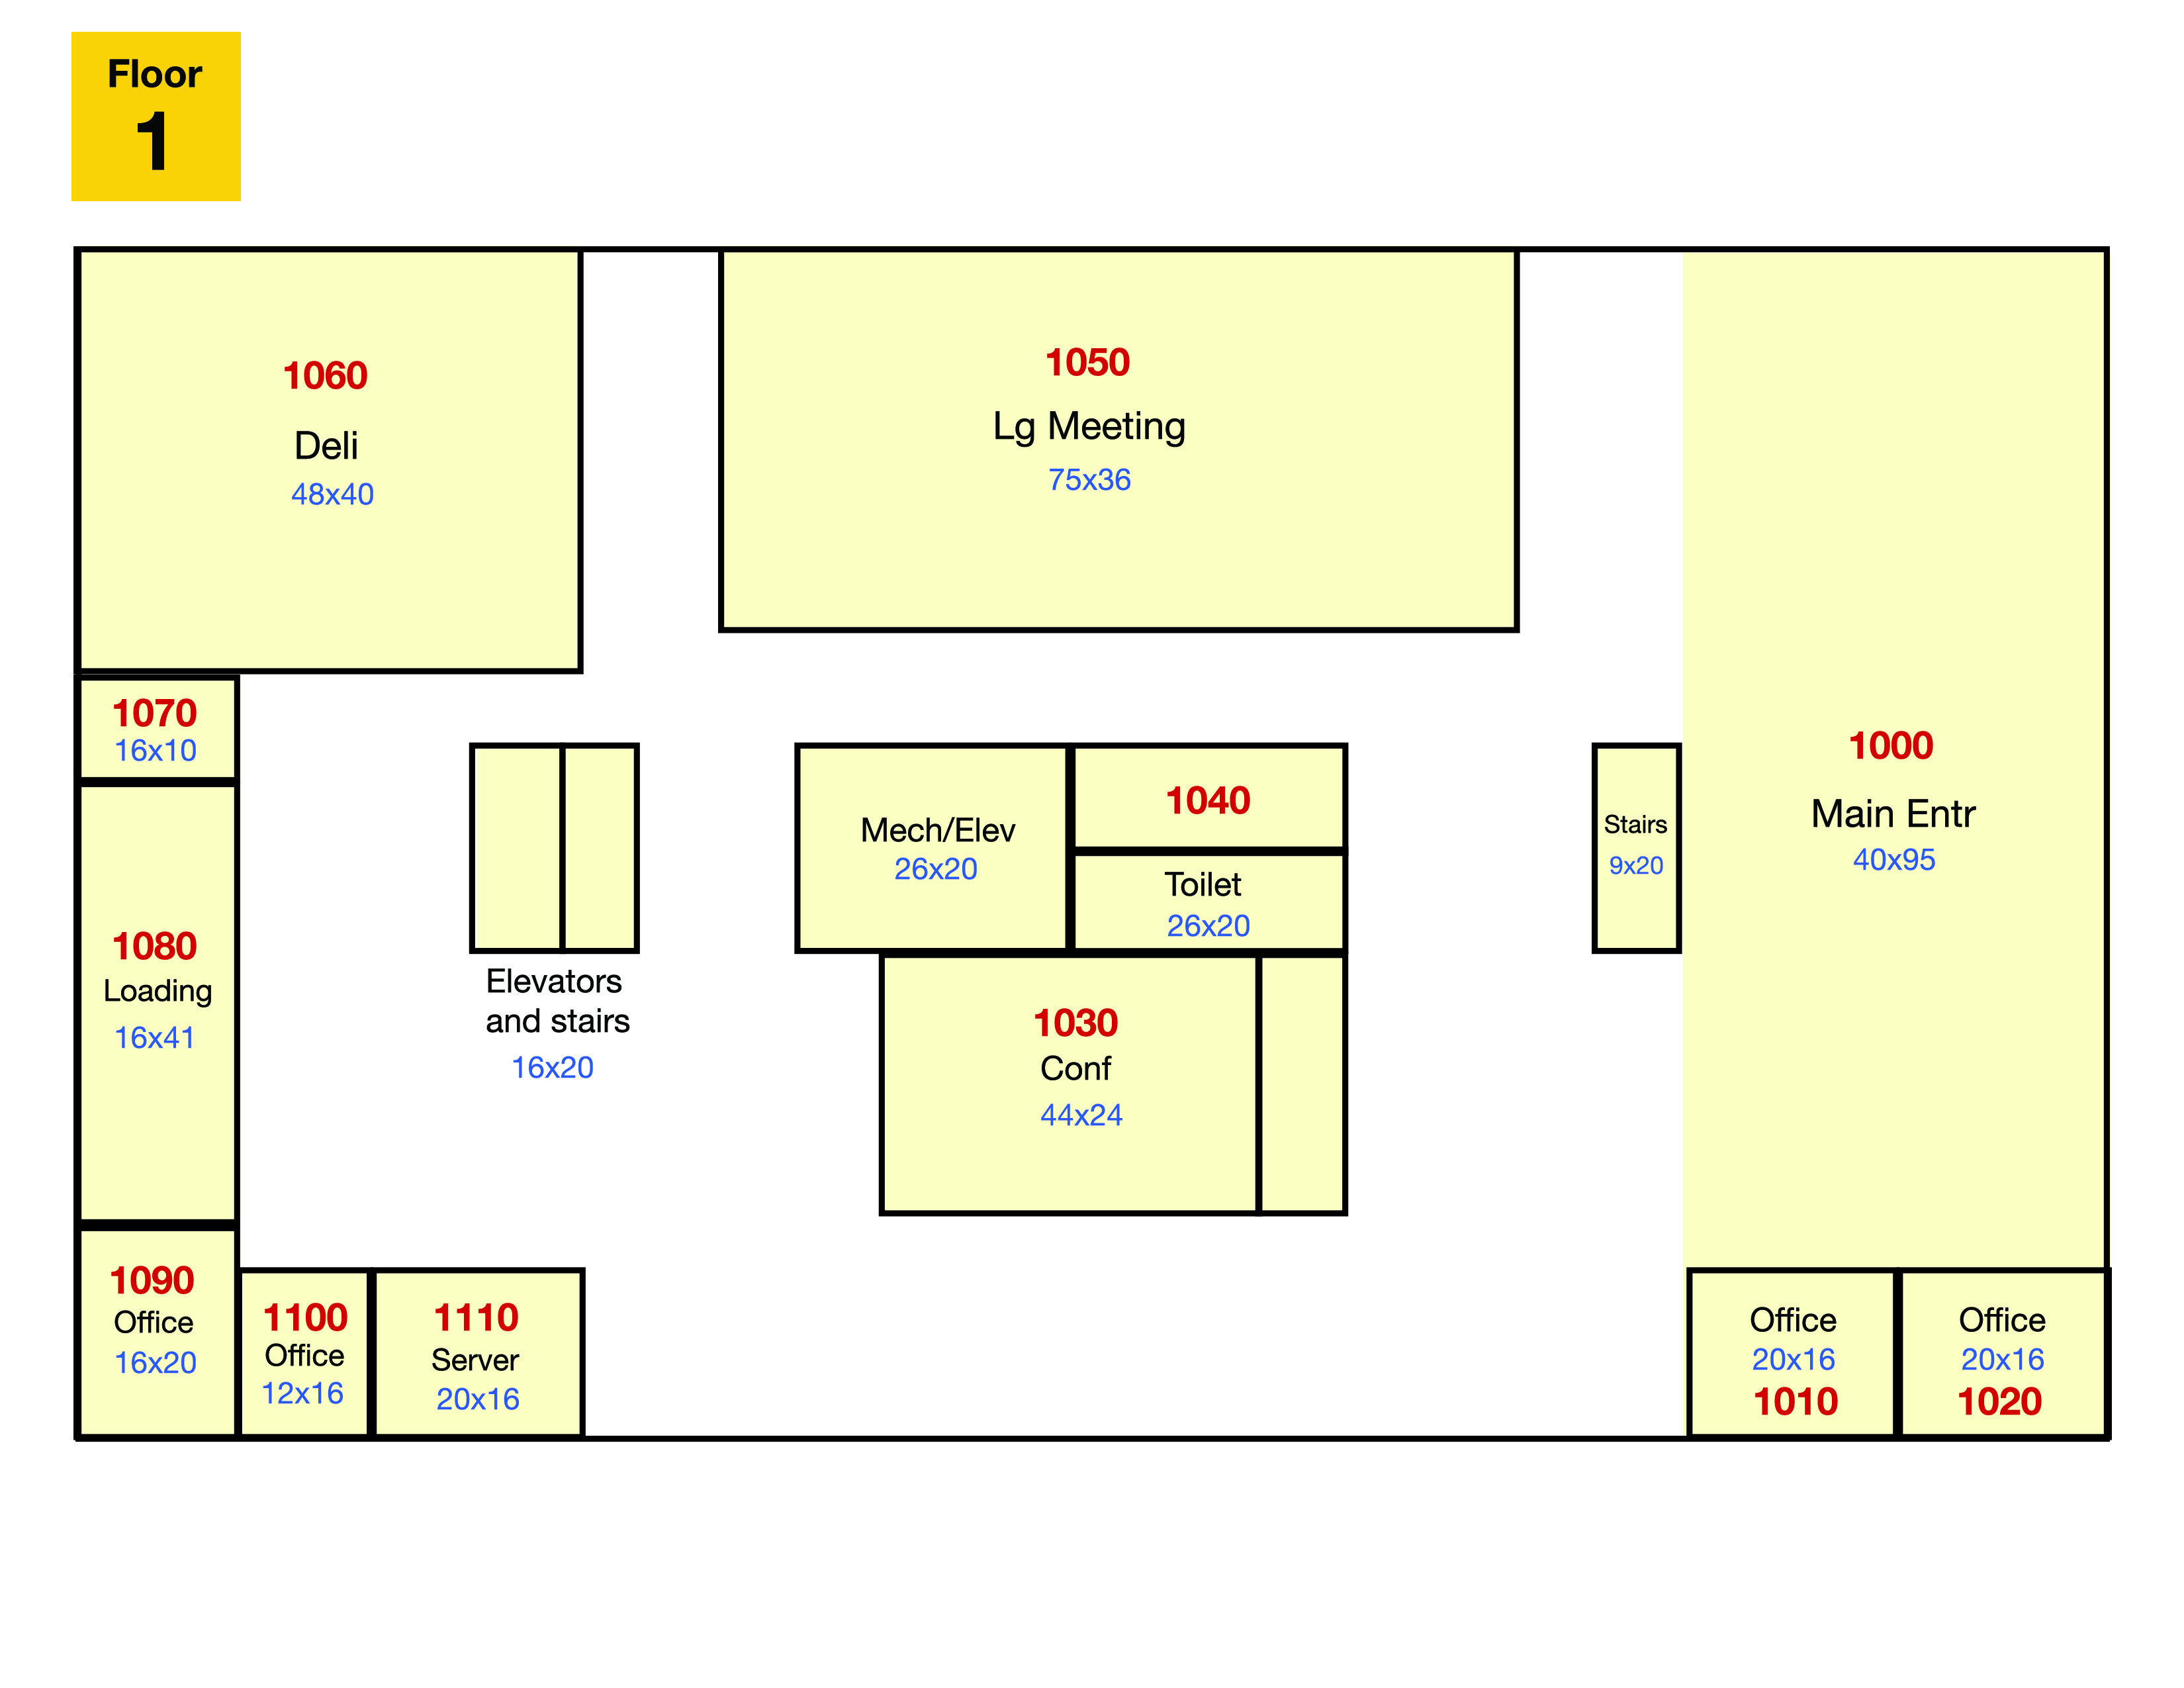
\includegraphics[width=0.3 \linewidth]{figures/basic1.jpg}
                        &
                        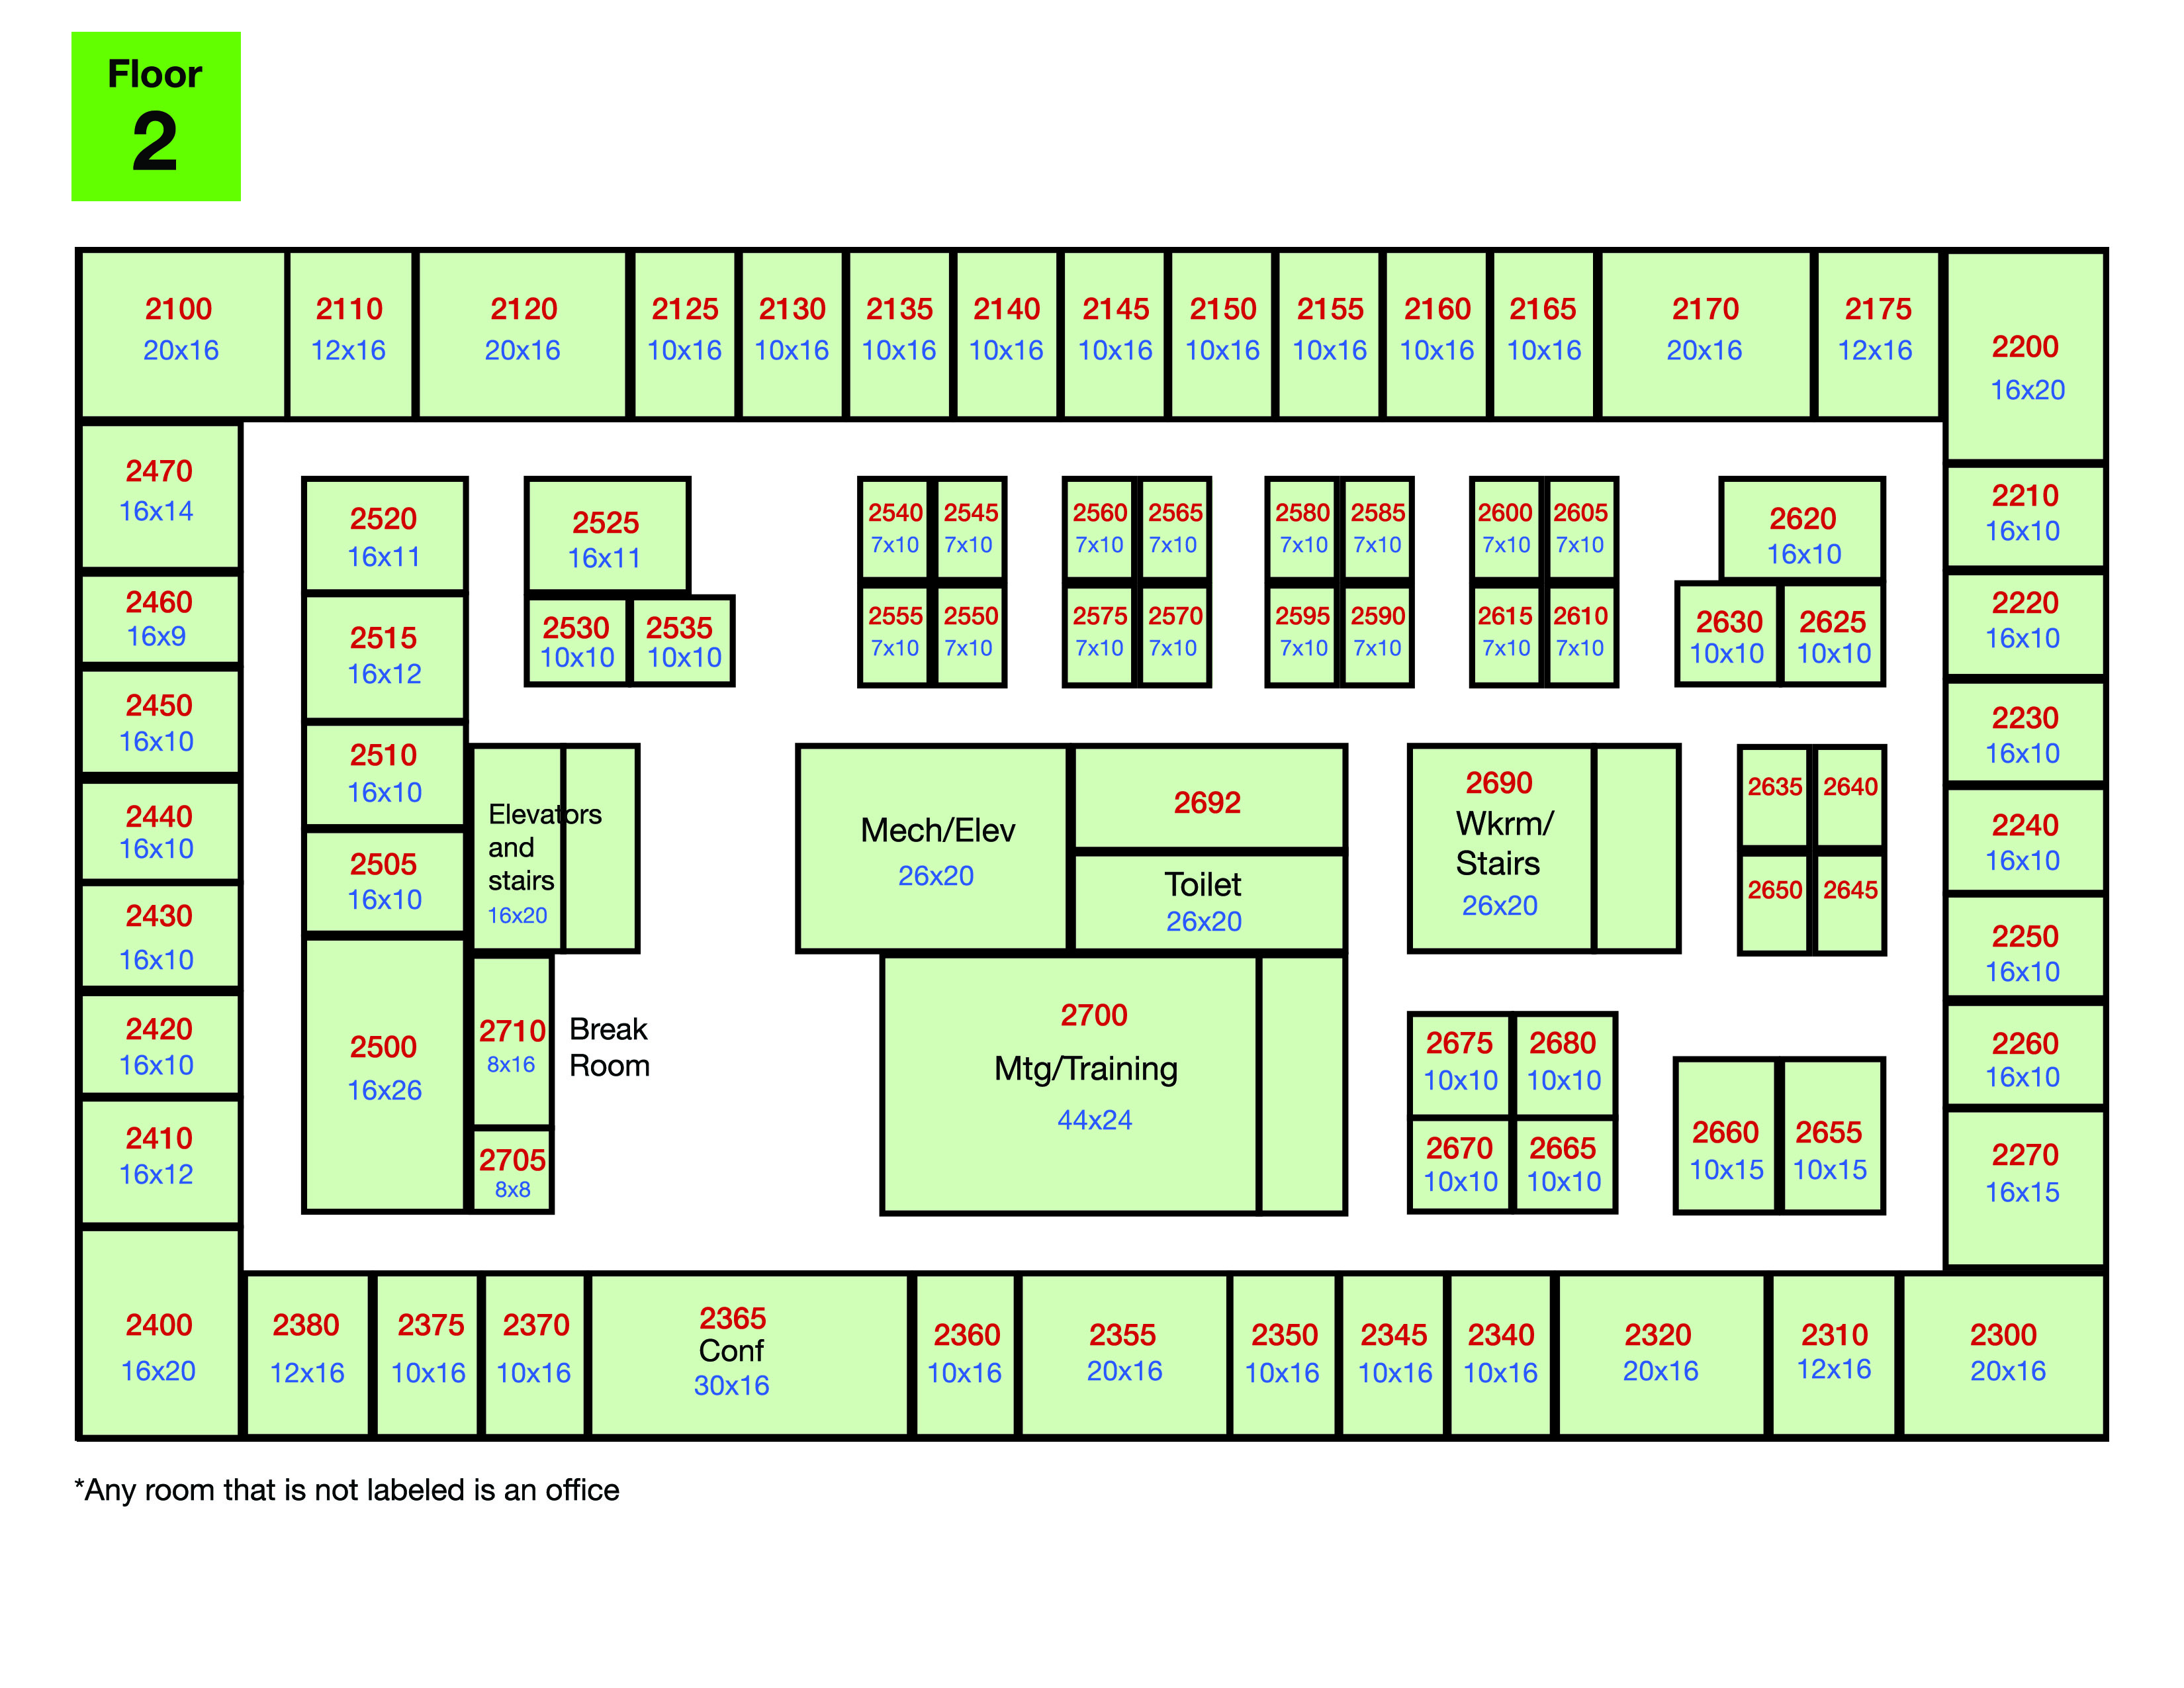
\includegraphics[width=0.3 \linewidth]{figures/basic2.jpg}
                        &
                        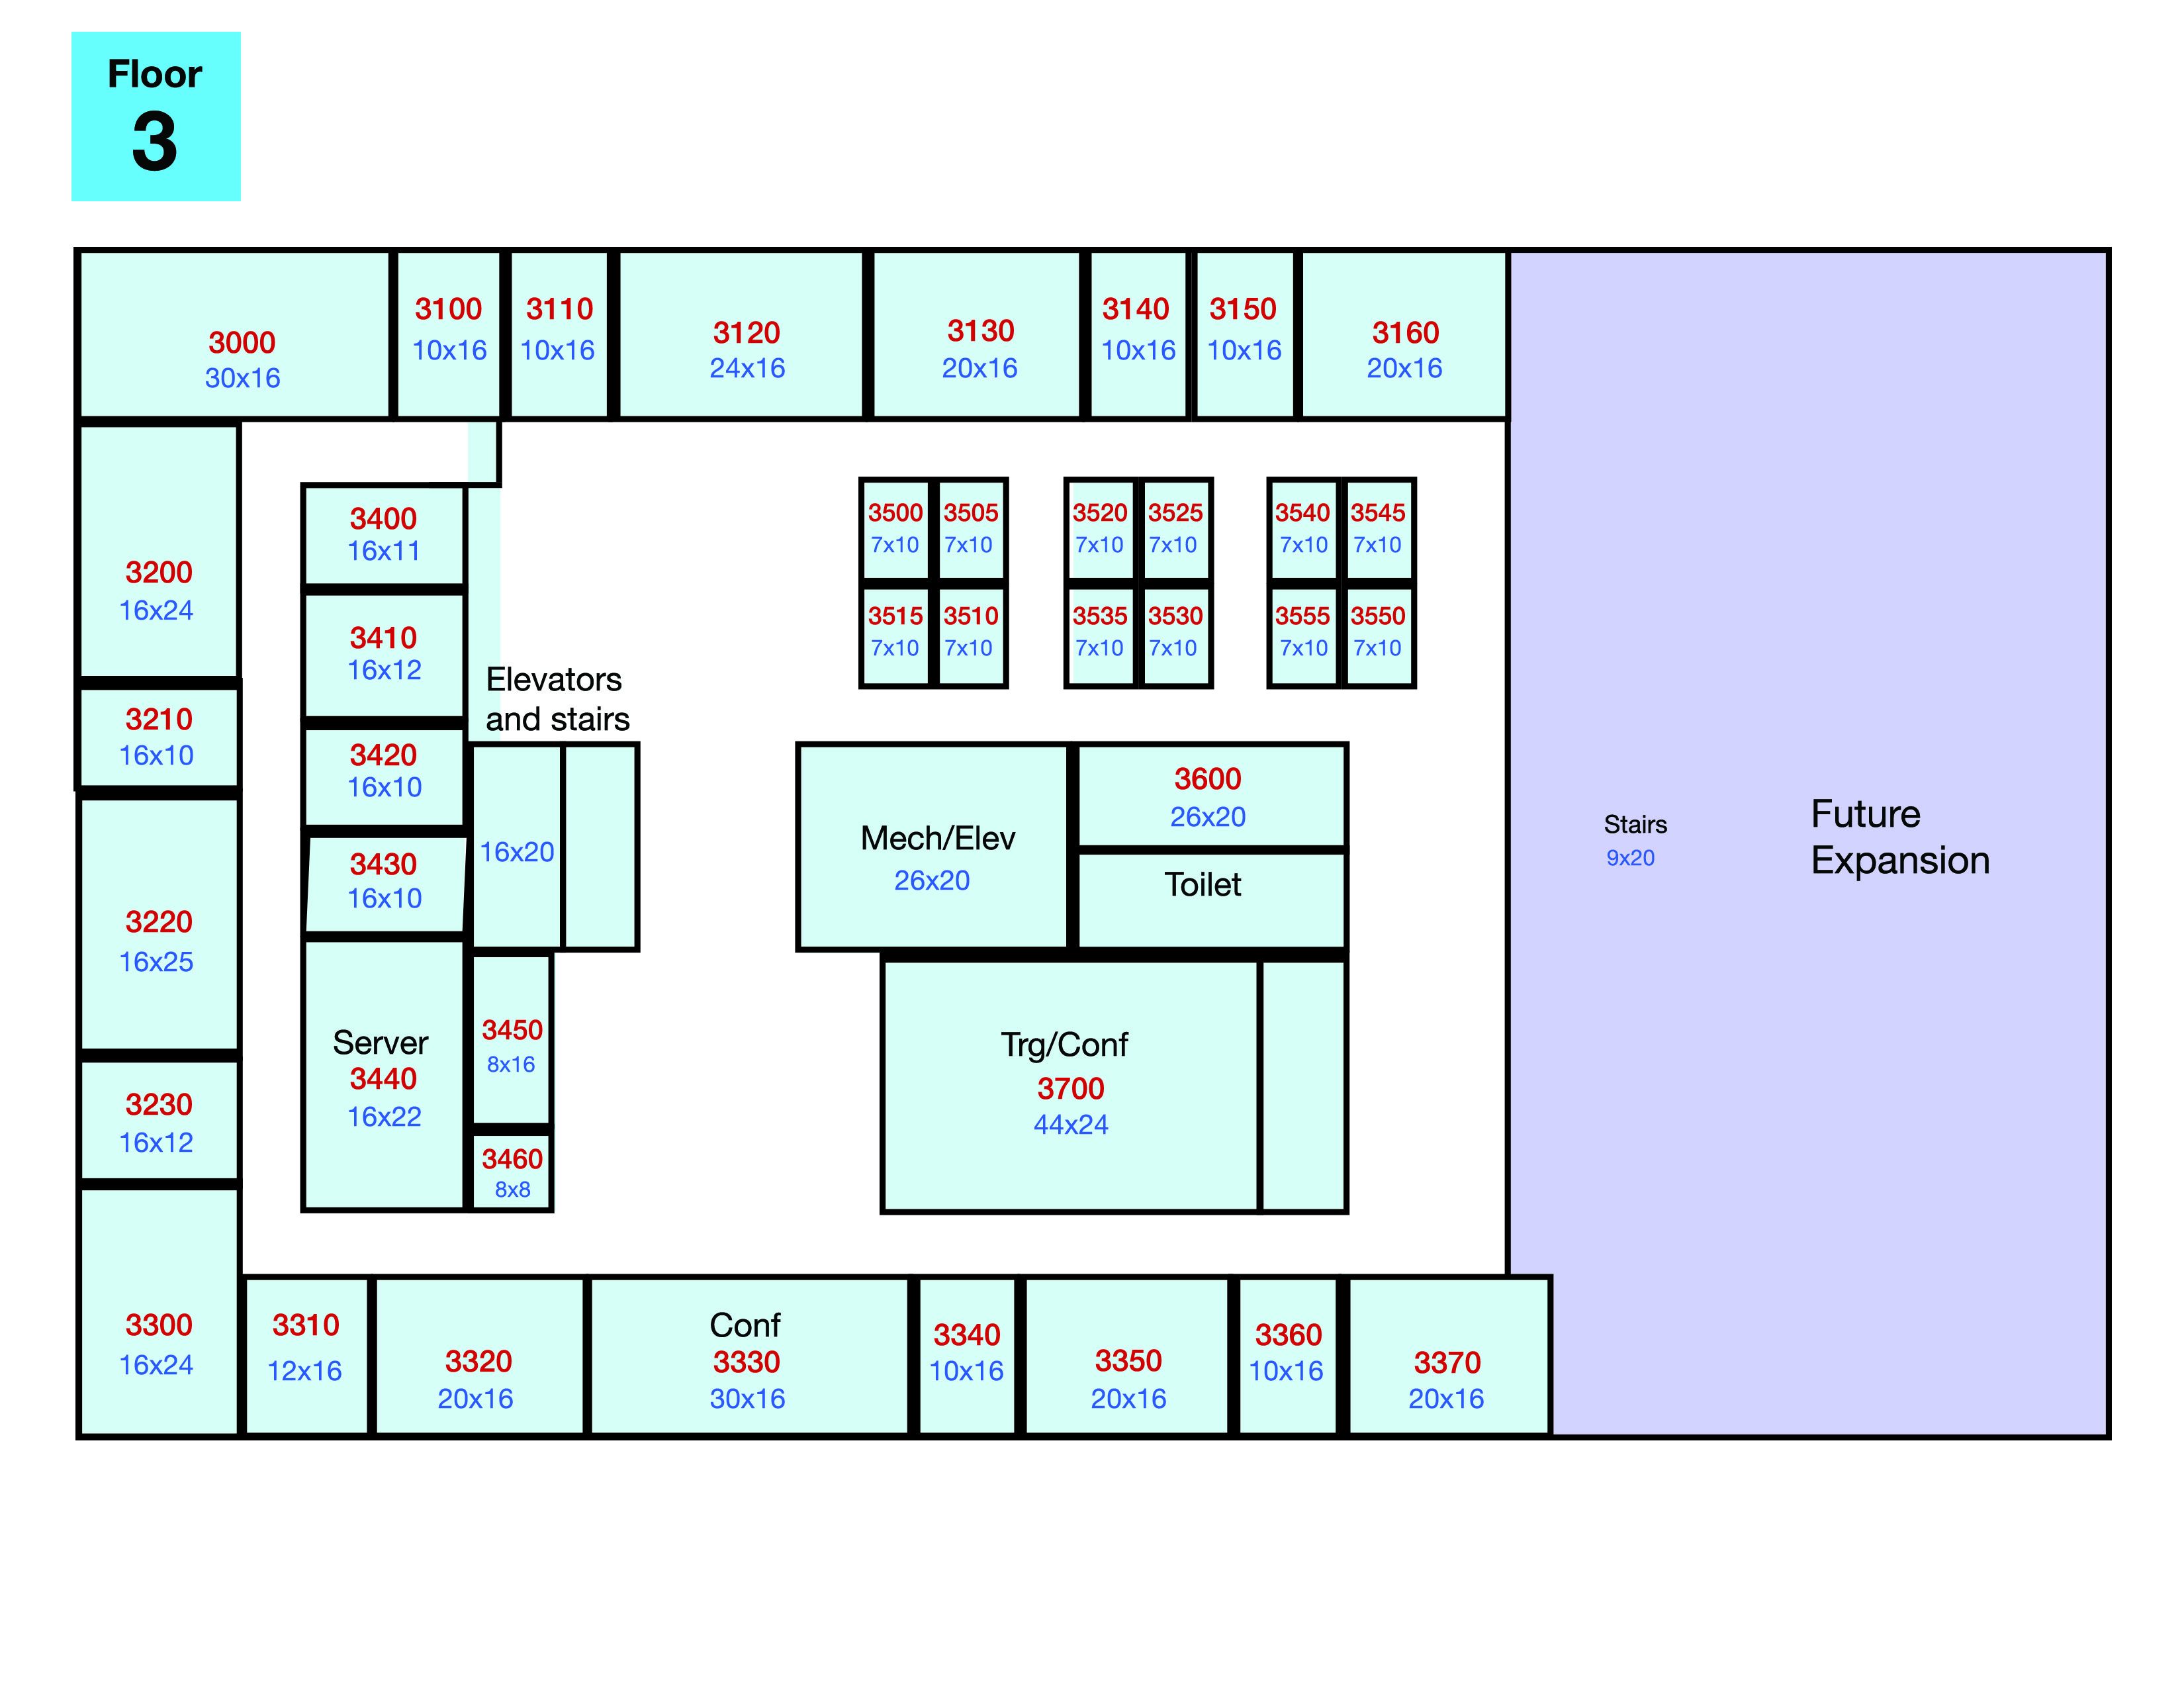
\includegraphics[width=0.3 \linewidth]{figures/basic3.jpg}
                        \\
                        
                        \mbox{(a) First Floor} & \mbox{(b) Second Floor} & \mbox{(c) Third Floor} \\
                    \end{array}$
                    \caption{Main Layout of the building}
                    \label{fig:main}
                \end{figure}
            
                The main layout of this building is as figure \ref{fig:main}. 
                
            \subsubsection{Energy Zone Layout}
                \begin{figure}[htbp]
                    \centering
                    $\begin{array}{ccc}
                        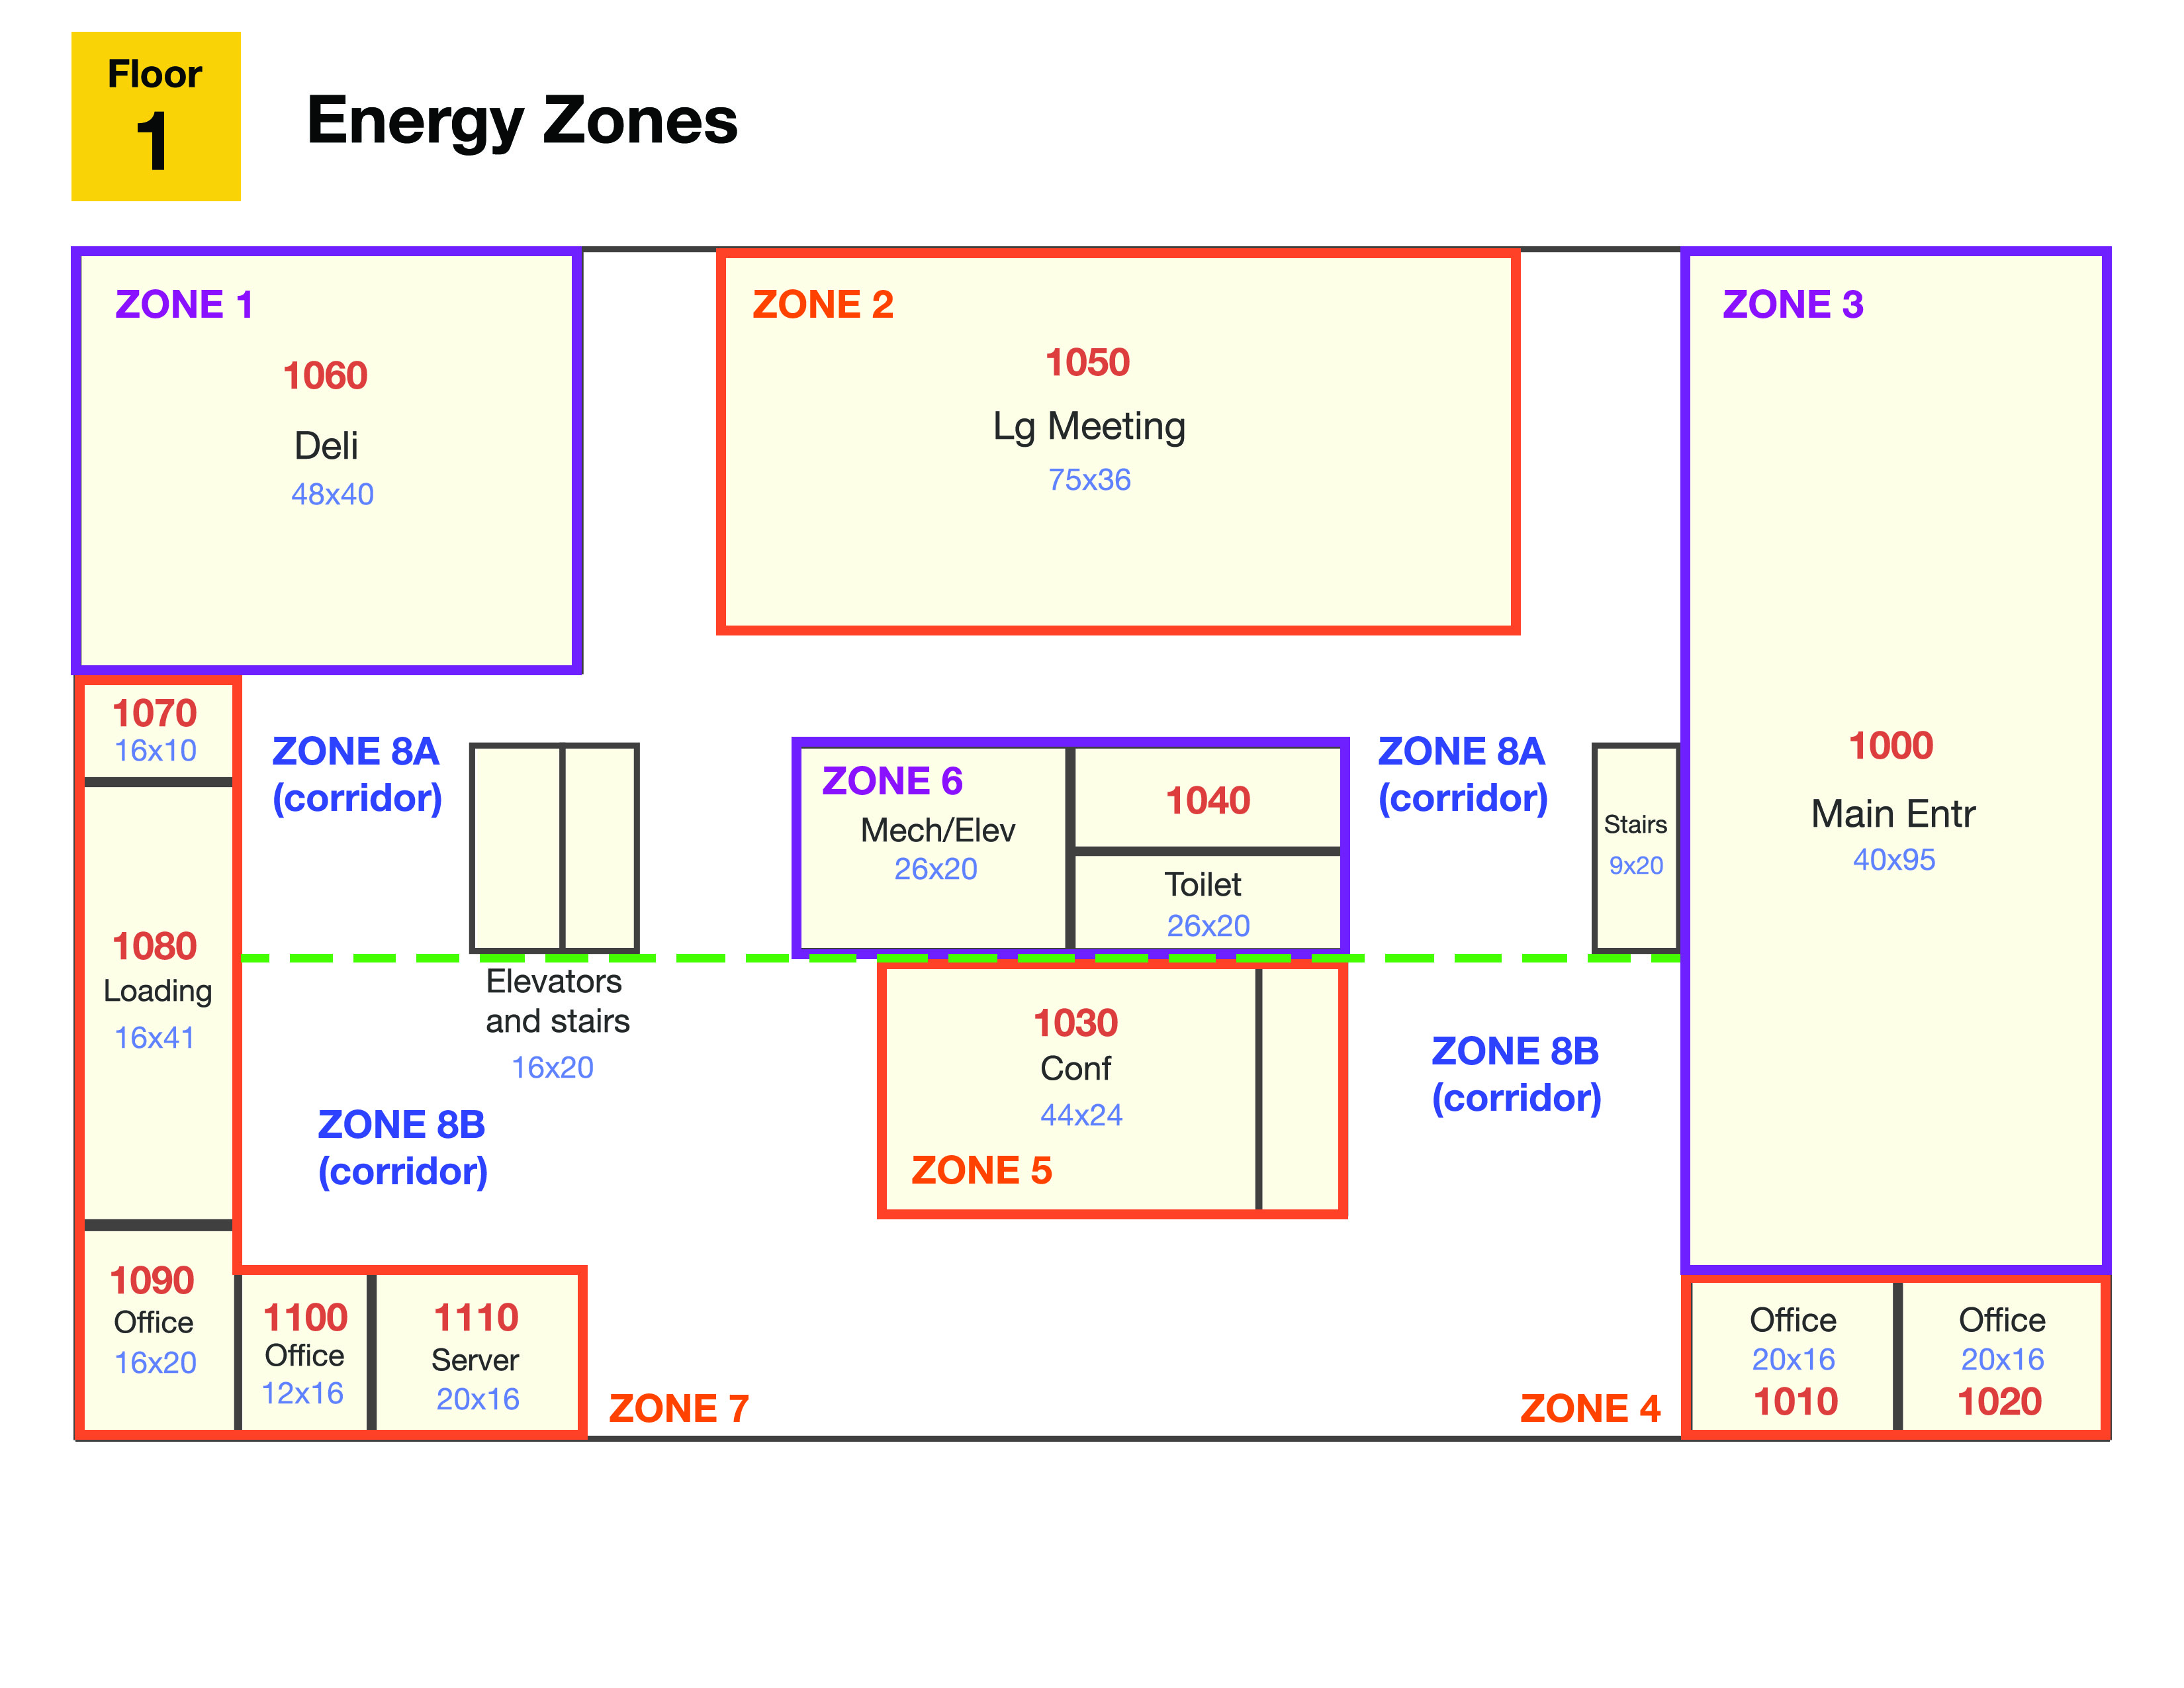
\includegraphics[width=0.3 \linewidth]{figures/energy1.jpg}
                        &
                        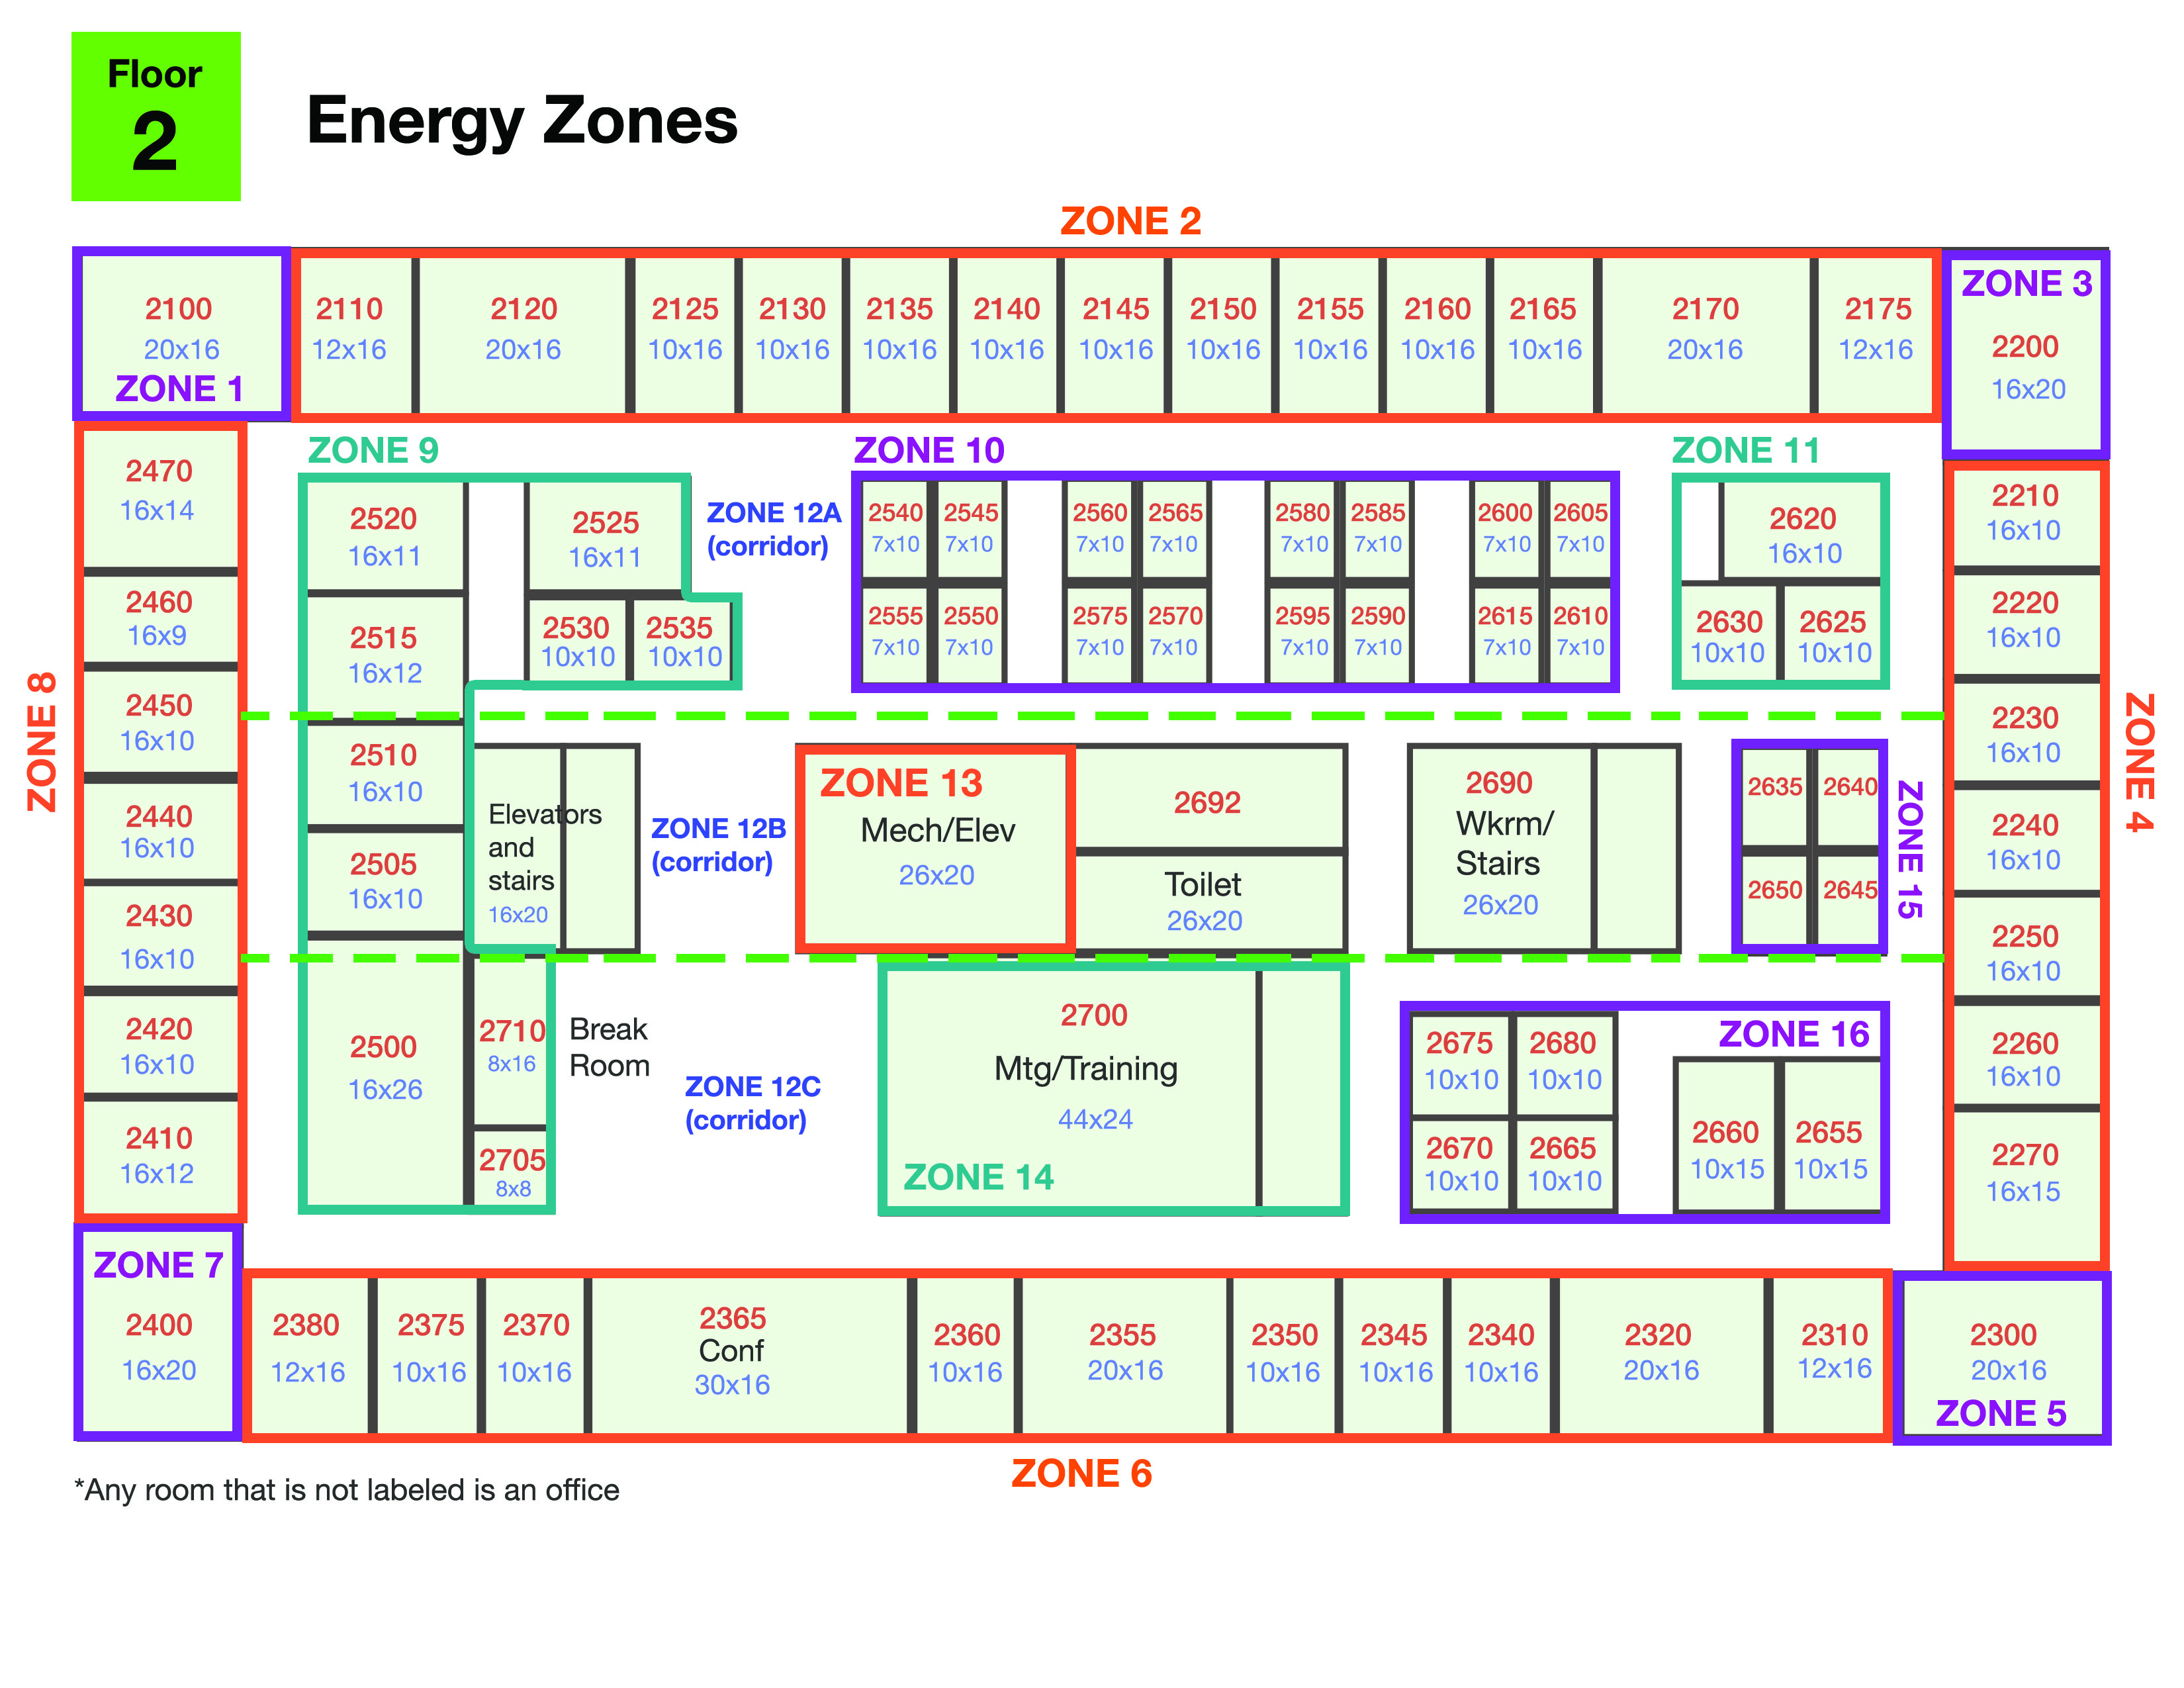
\includegraphics[width=0.3 \linewidth]{figures/energy2.jpg}
                        &
                        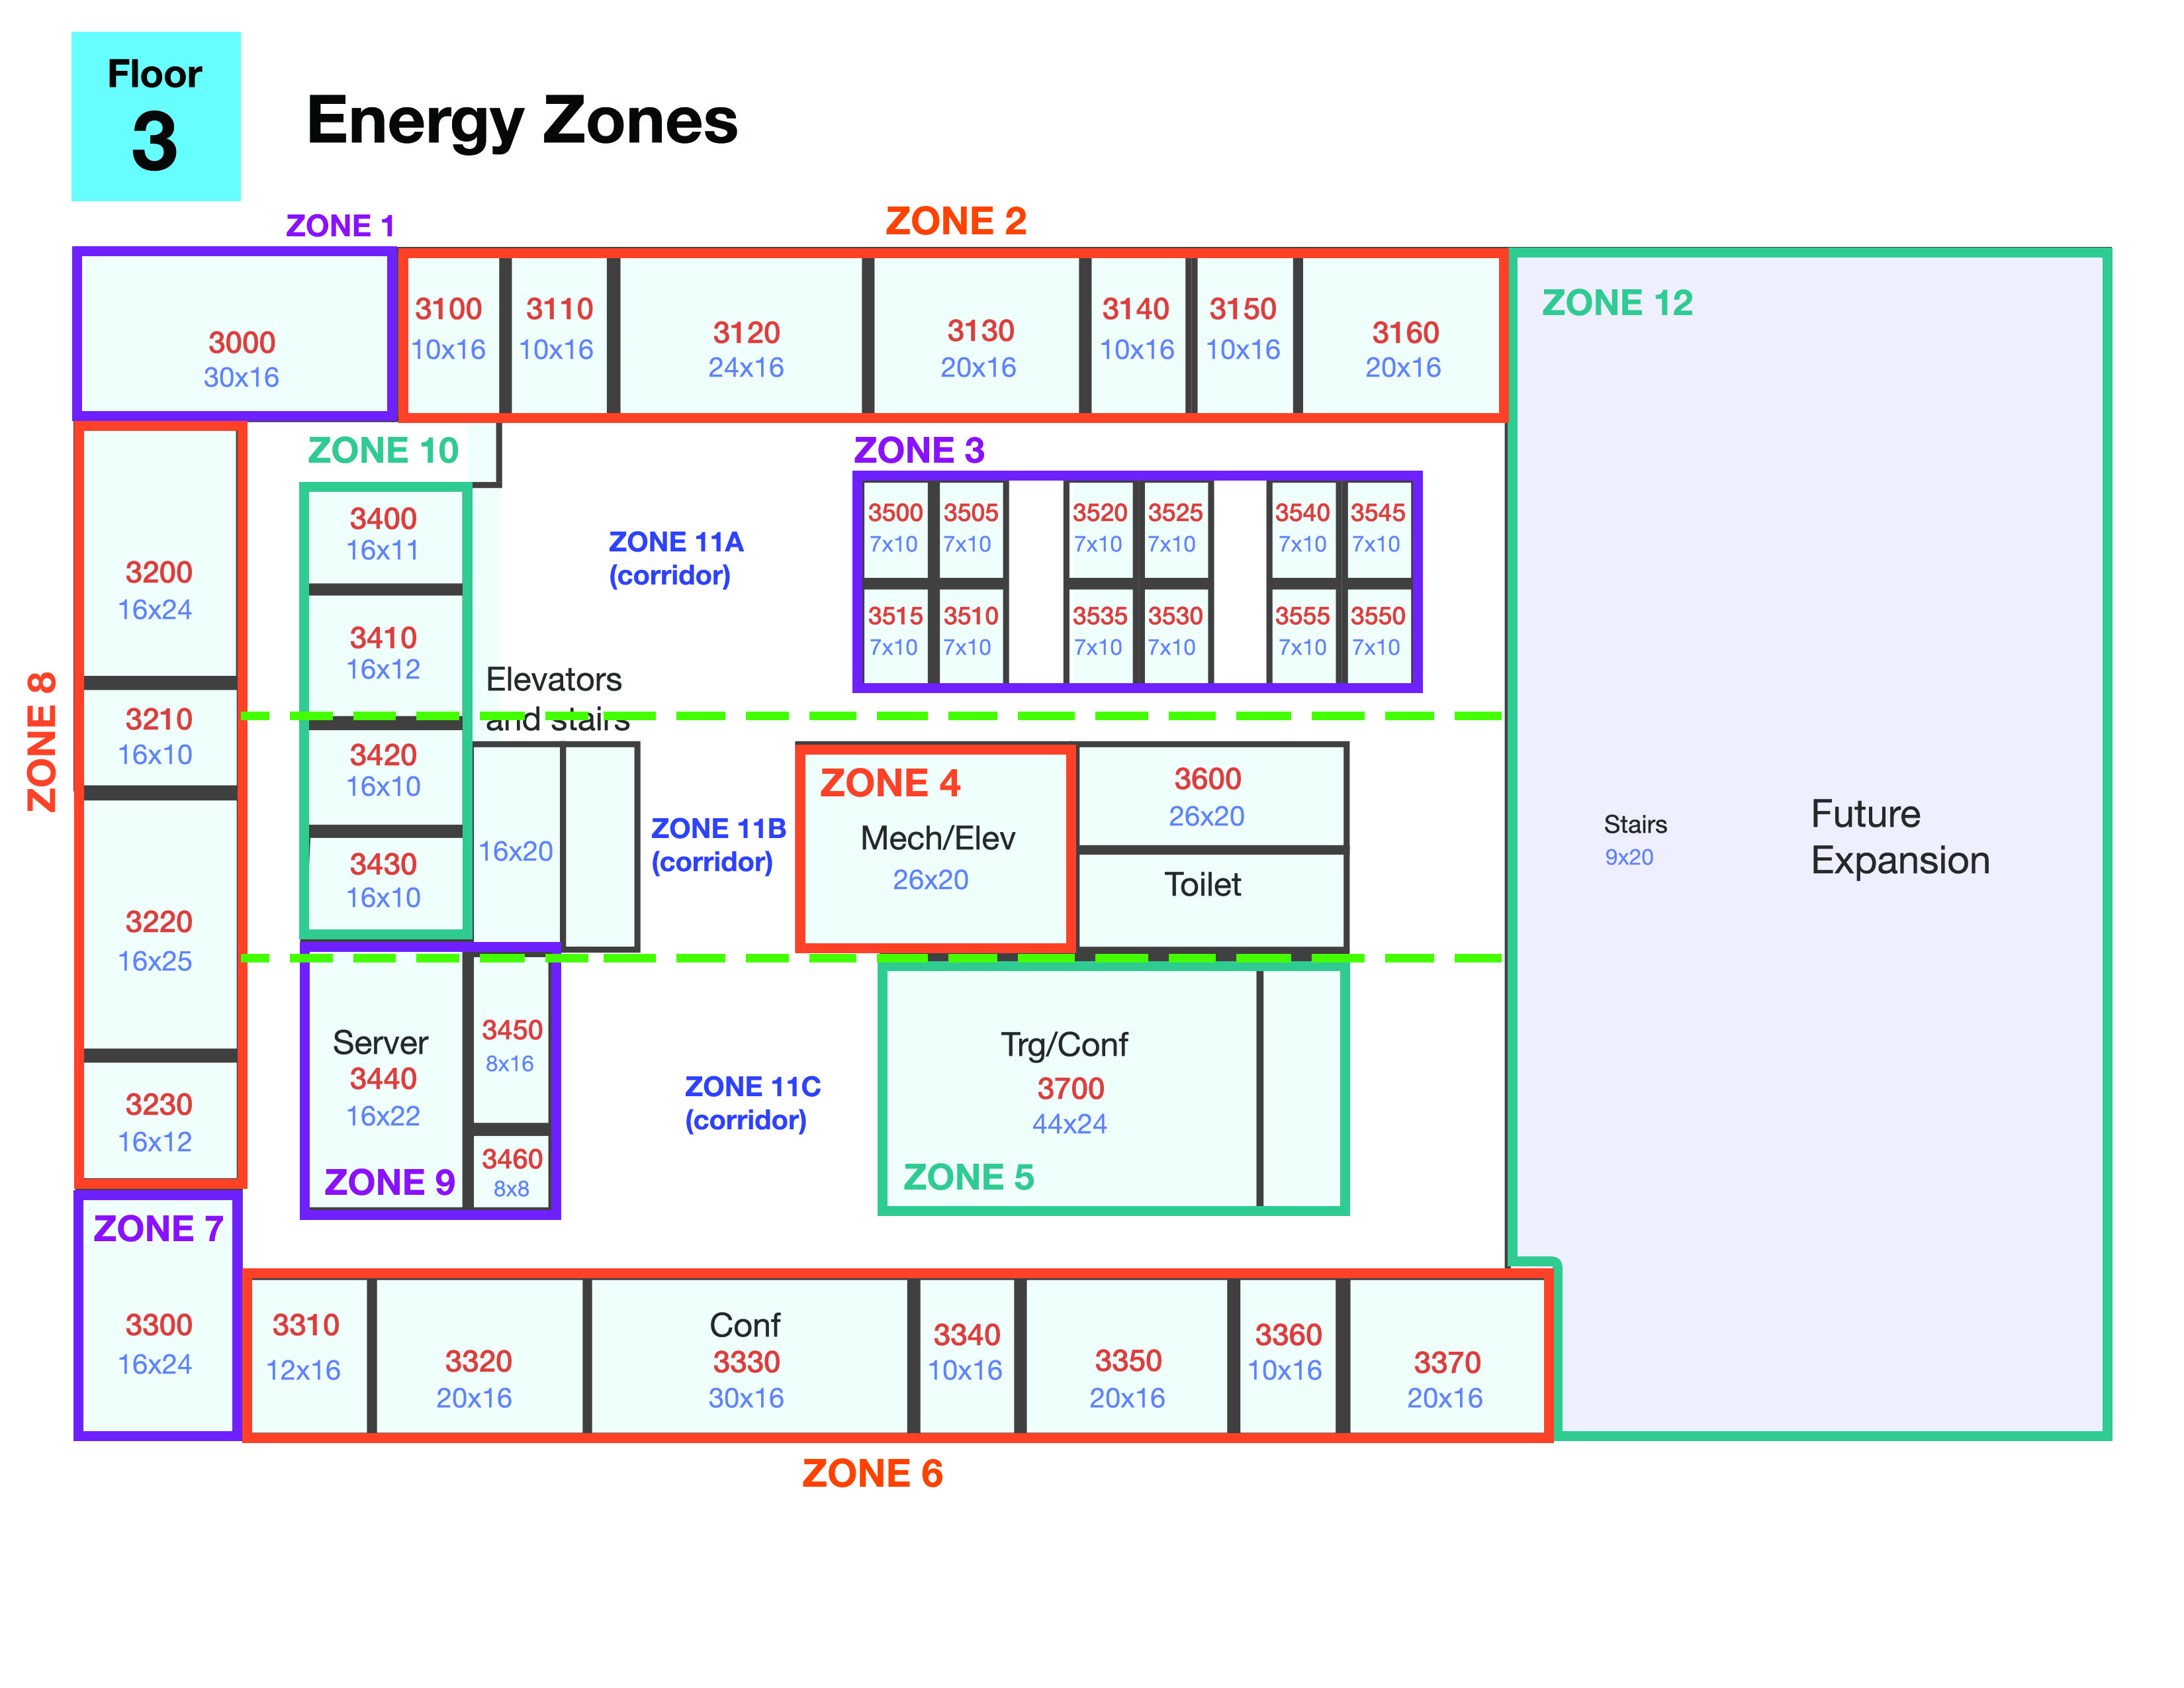
\includegraphics[width=0.3 \linewidth]{figures/energy3.jpg}
                        \\
                        
                        \mbox{(a) First Floor} & \mbox{(b) Second Floor} & \mbox{(c) Third Floor} \\
                    \end{array}$
                    \caption{Energy Zone of the Building}
                    \label{fig:energy}
                \end{figure}
            
                The energy zone of this building is as figure \ref{fig:energy}. 
                
            \subsubsection{Prox Zone Layout}
                \begin{figure}[htbp]
                    \centering
                    $\begin{array}{ccc}
                        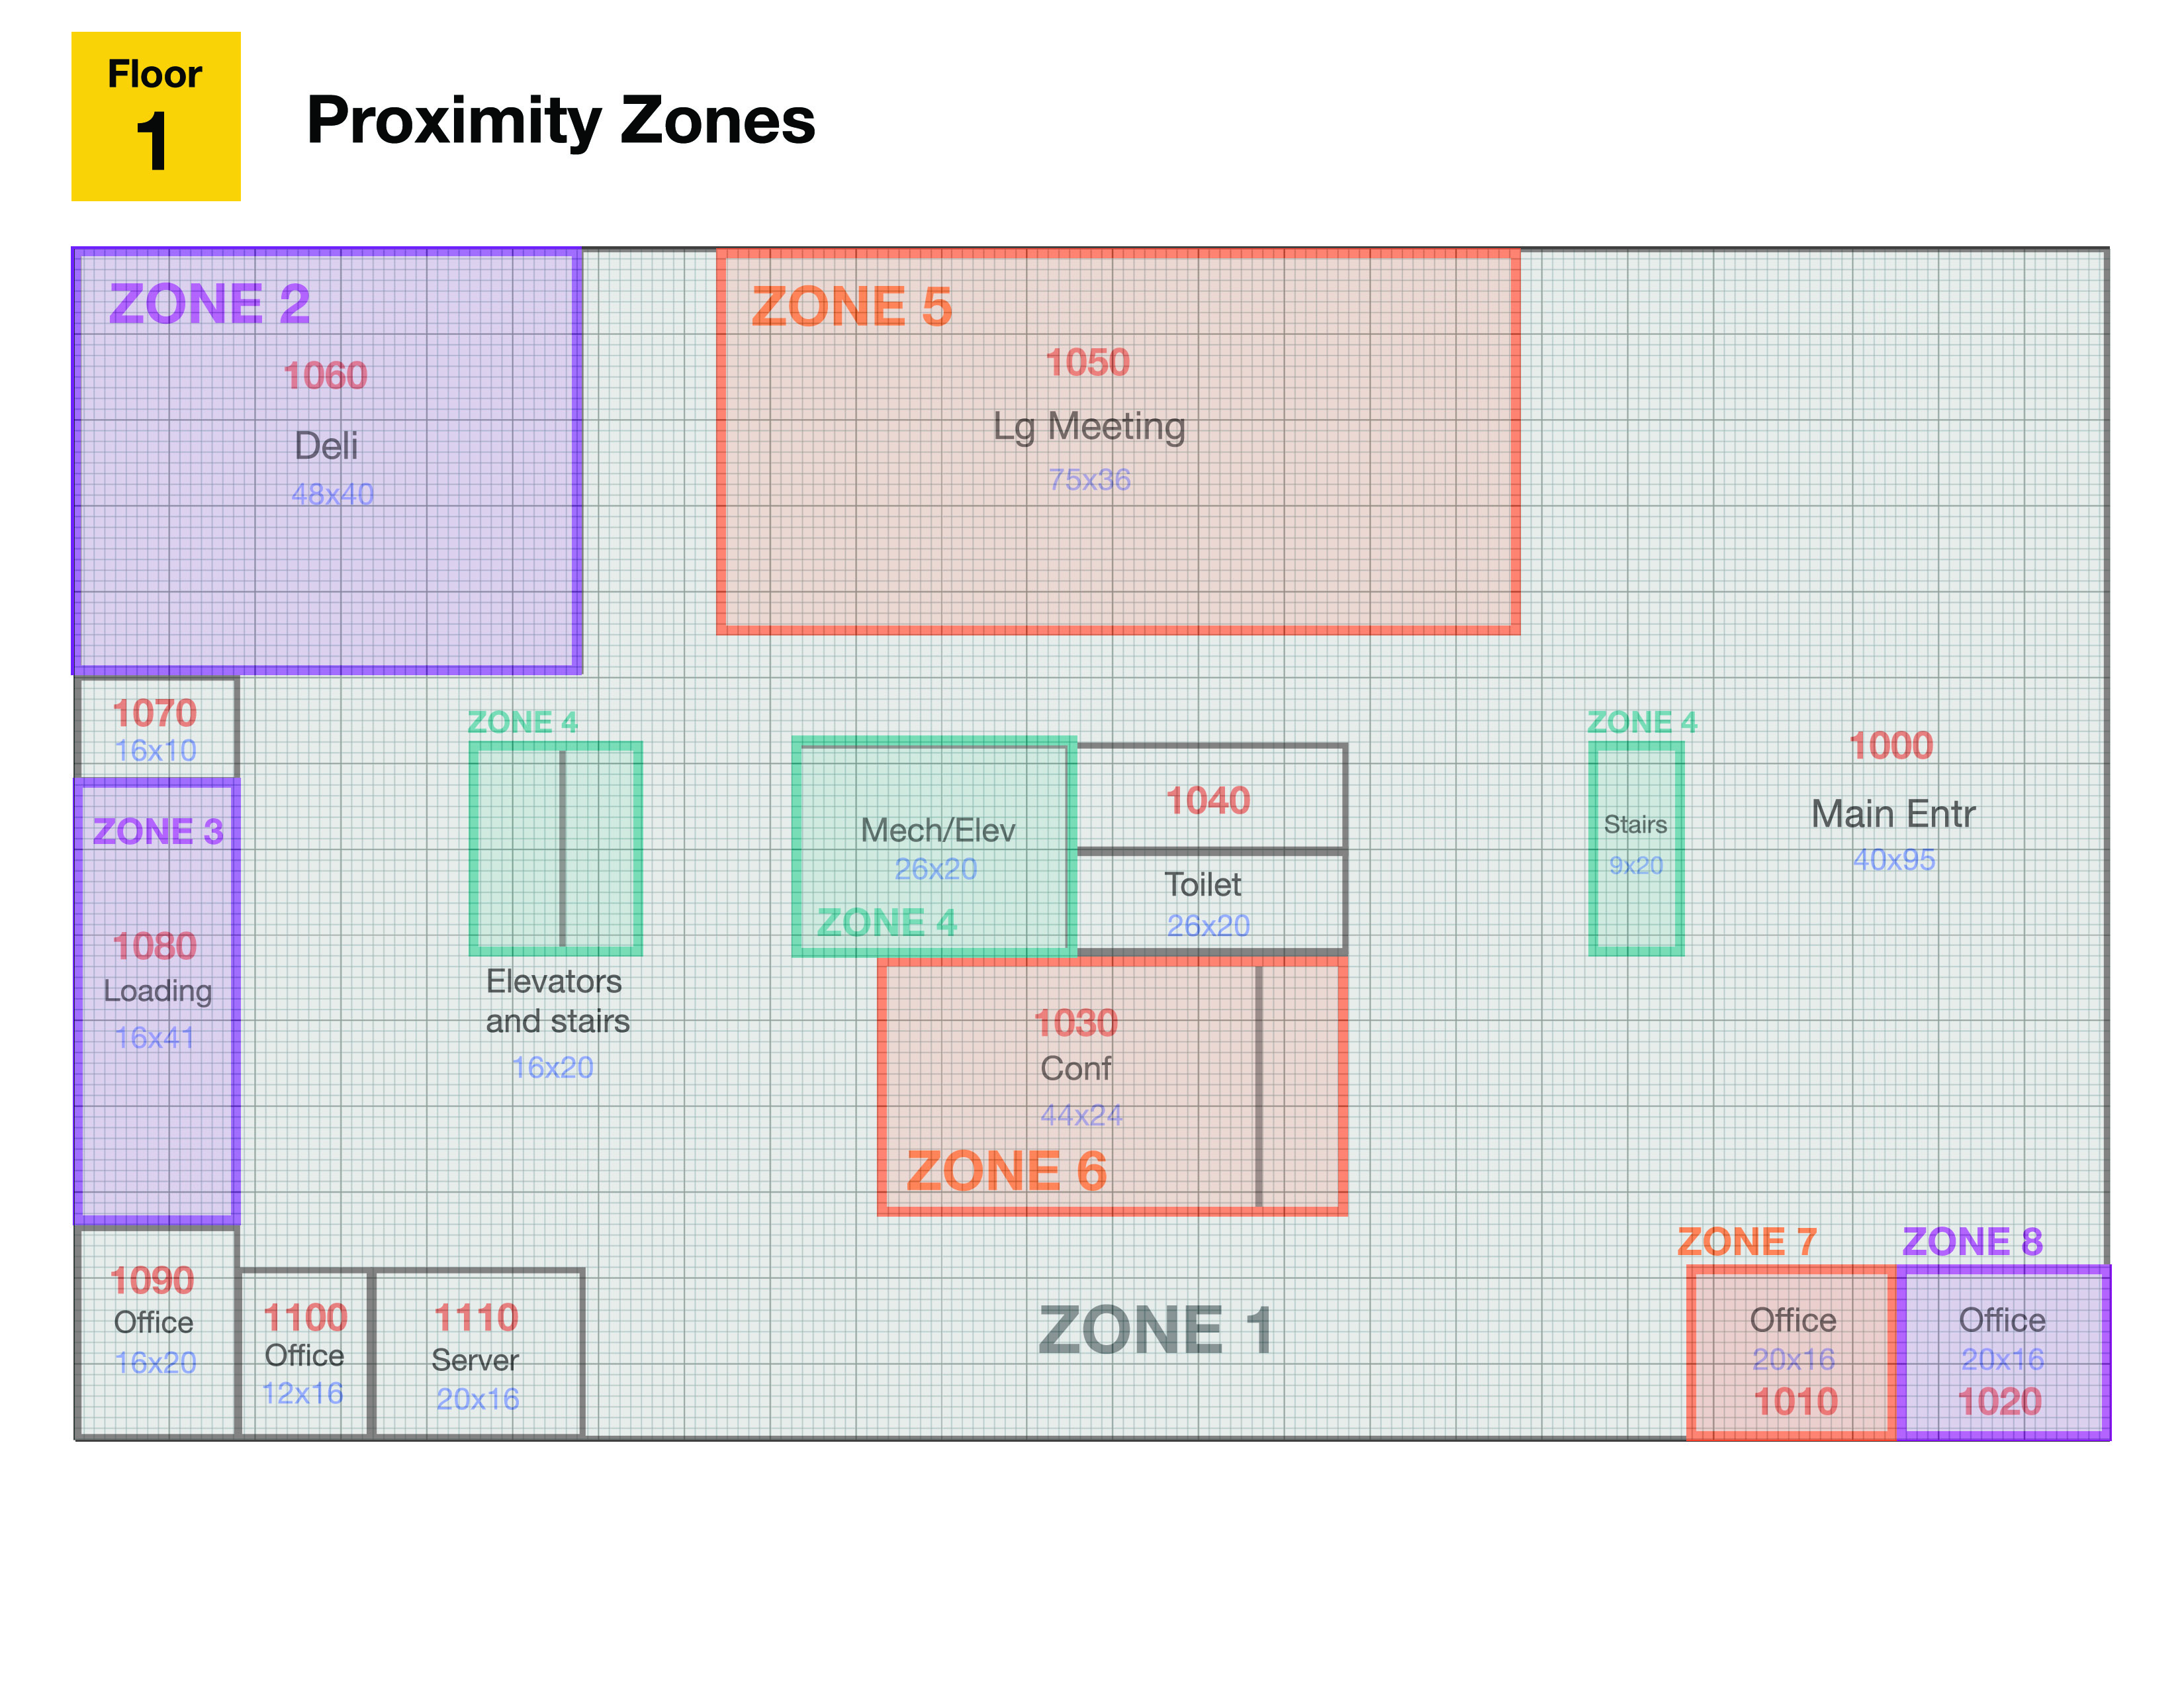
\includegraphics[width=0.3 \linewidth]{figures/prox1.jpg}
                        &
                        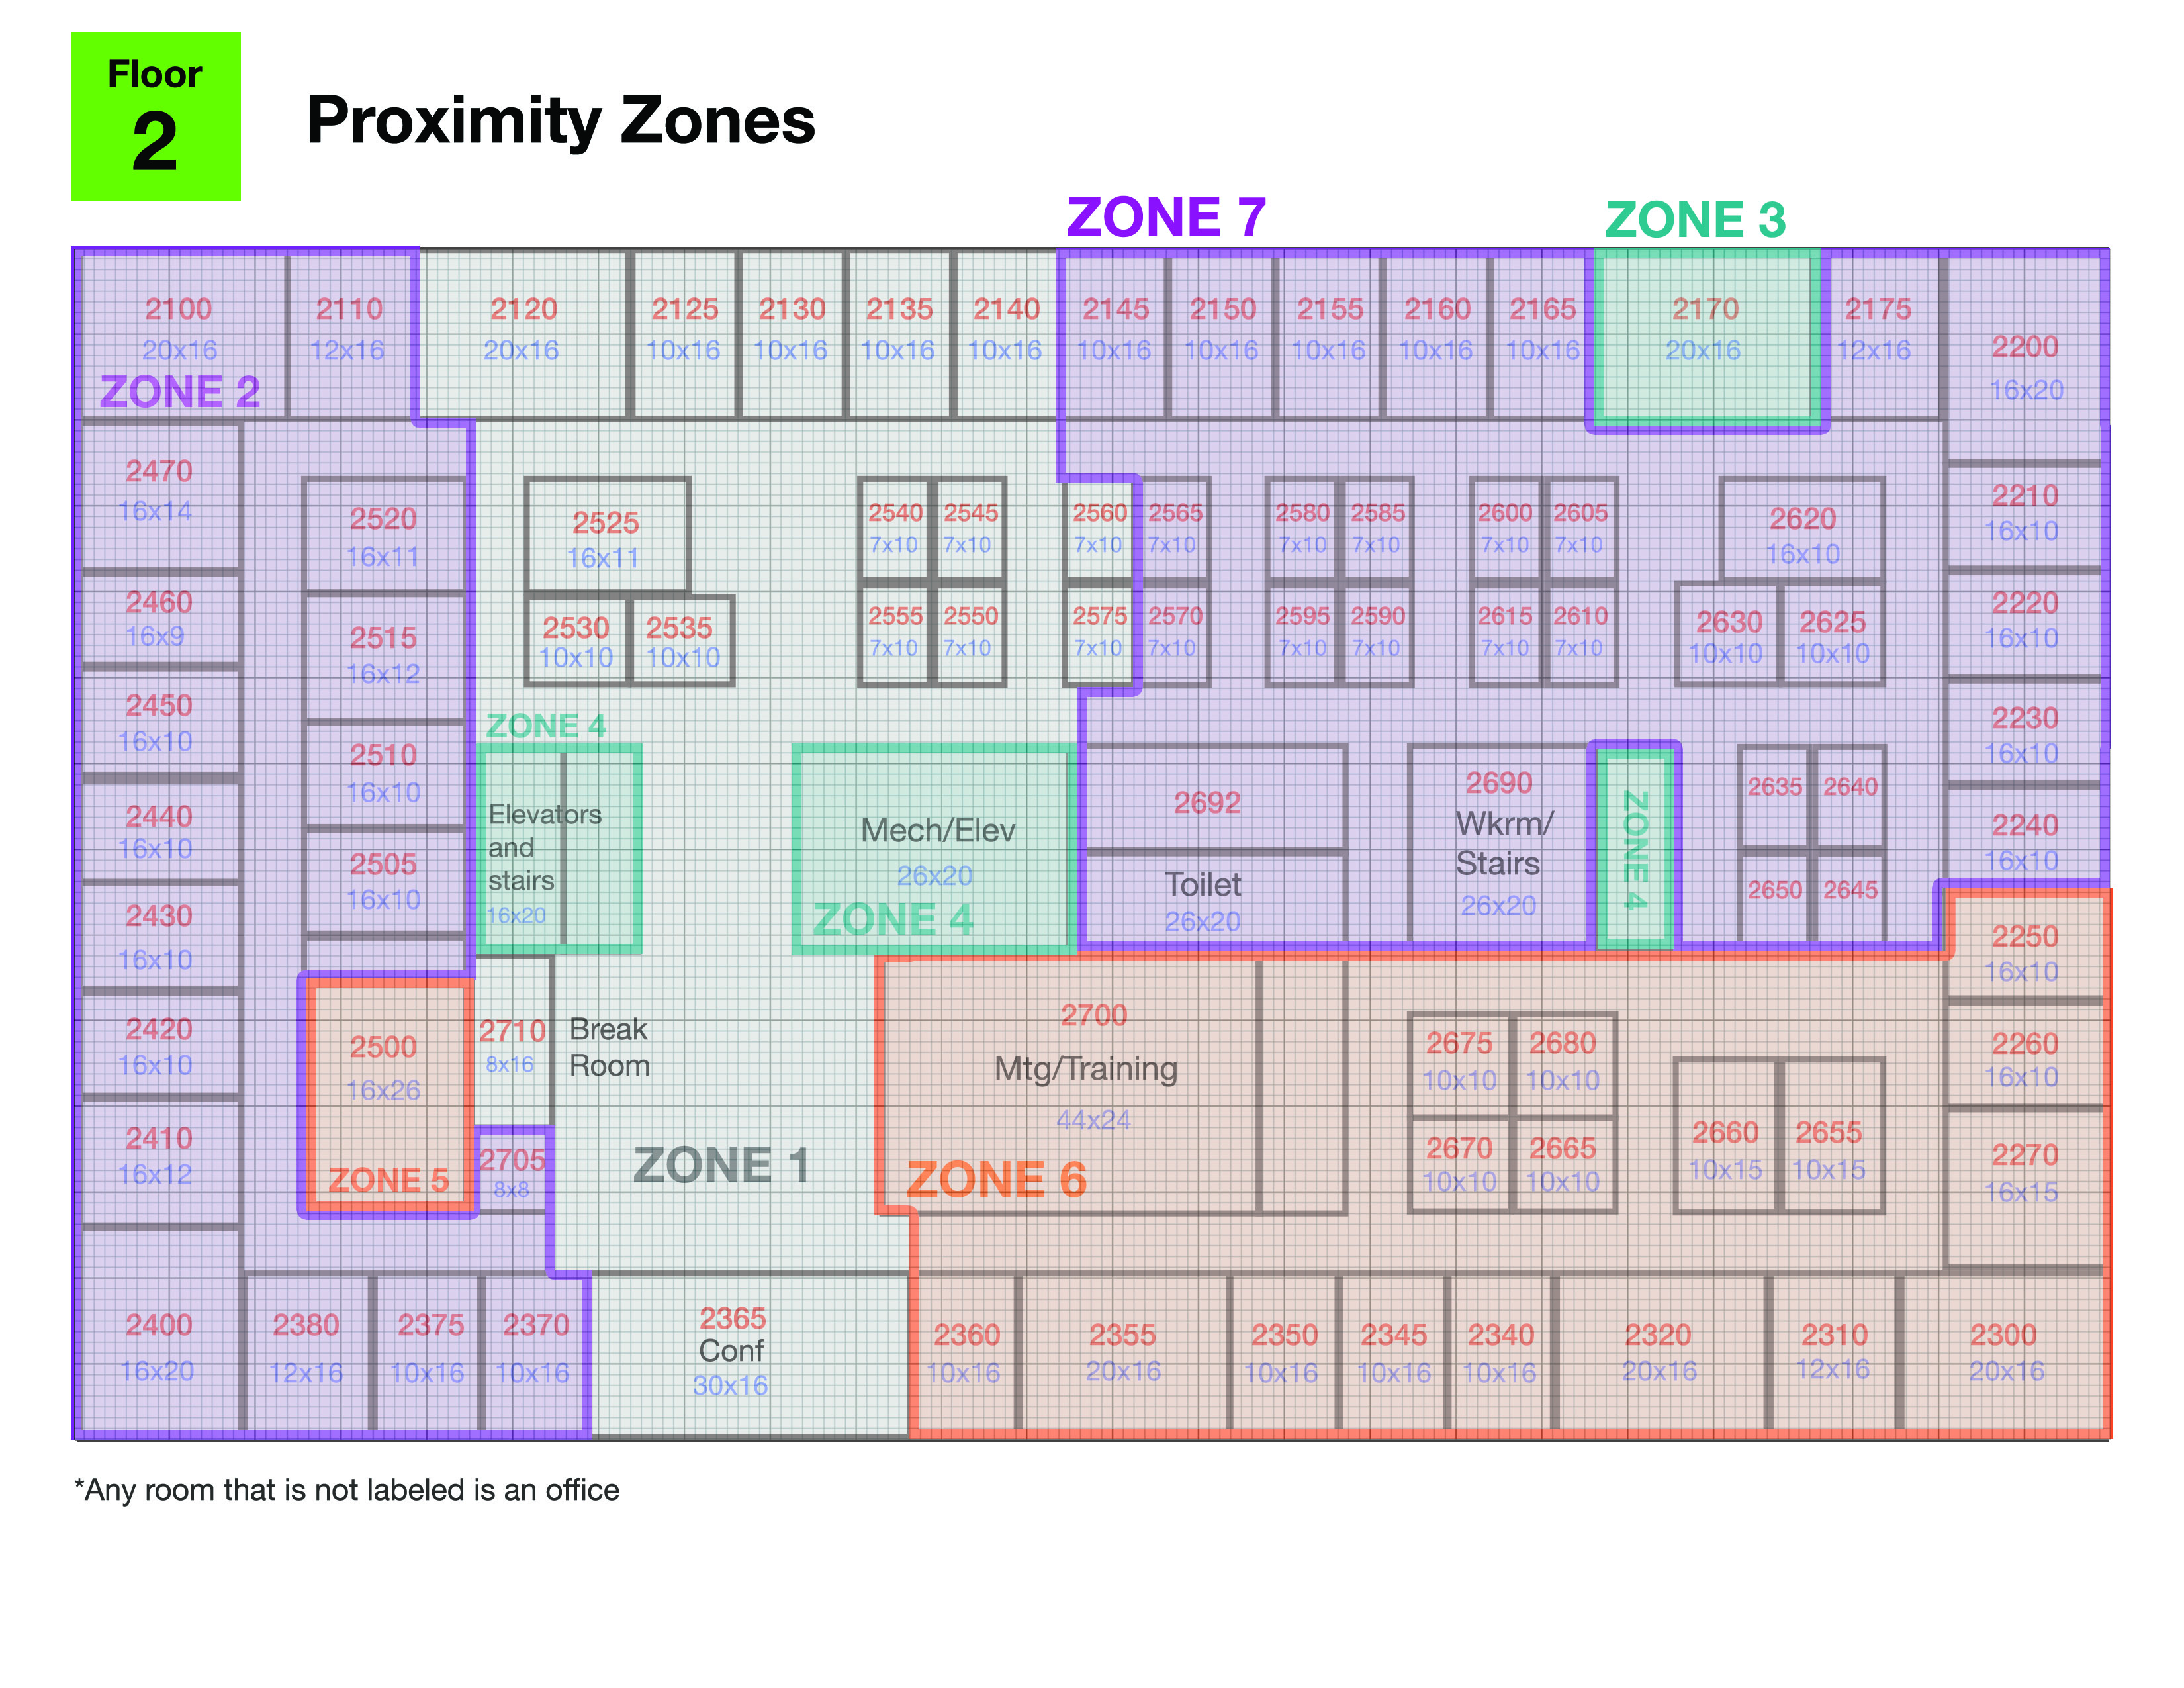
\includegraphics[width=0.3 \linewidth]{figures/prox2.jpg}
                        &
                        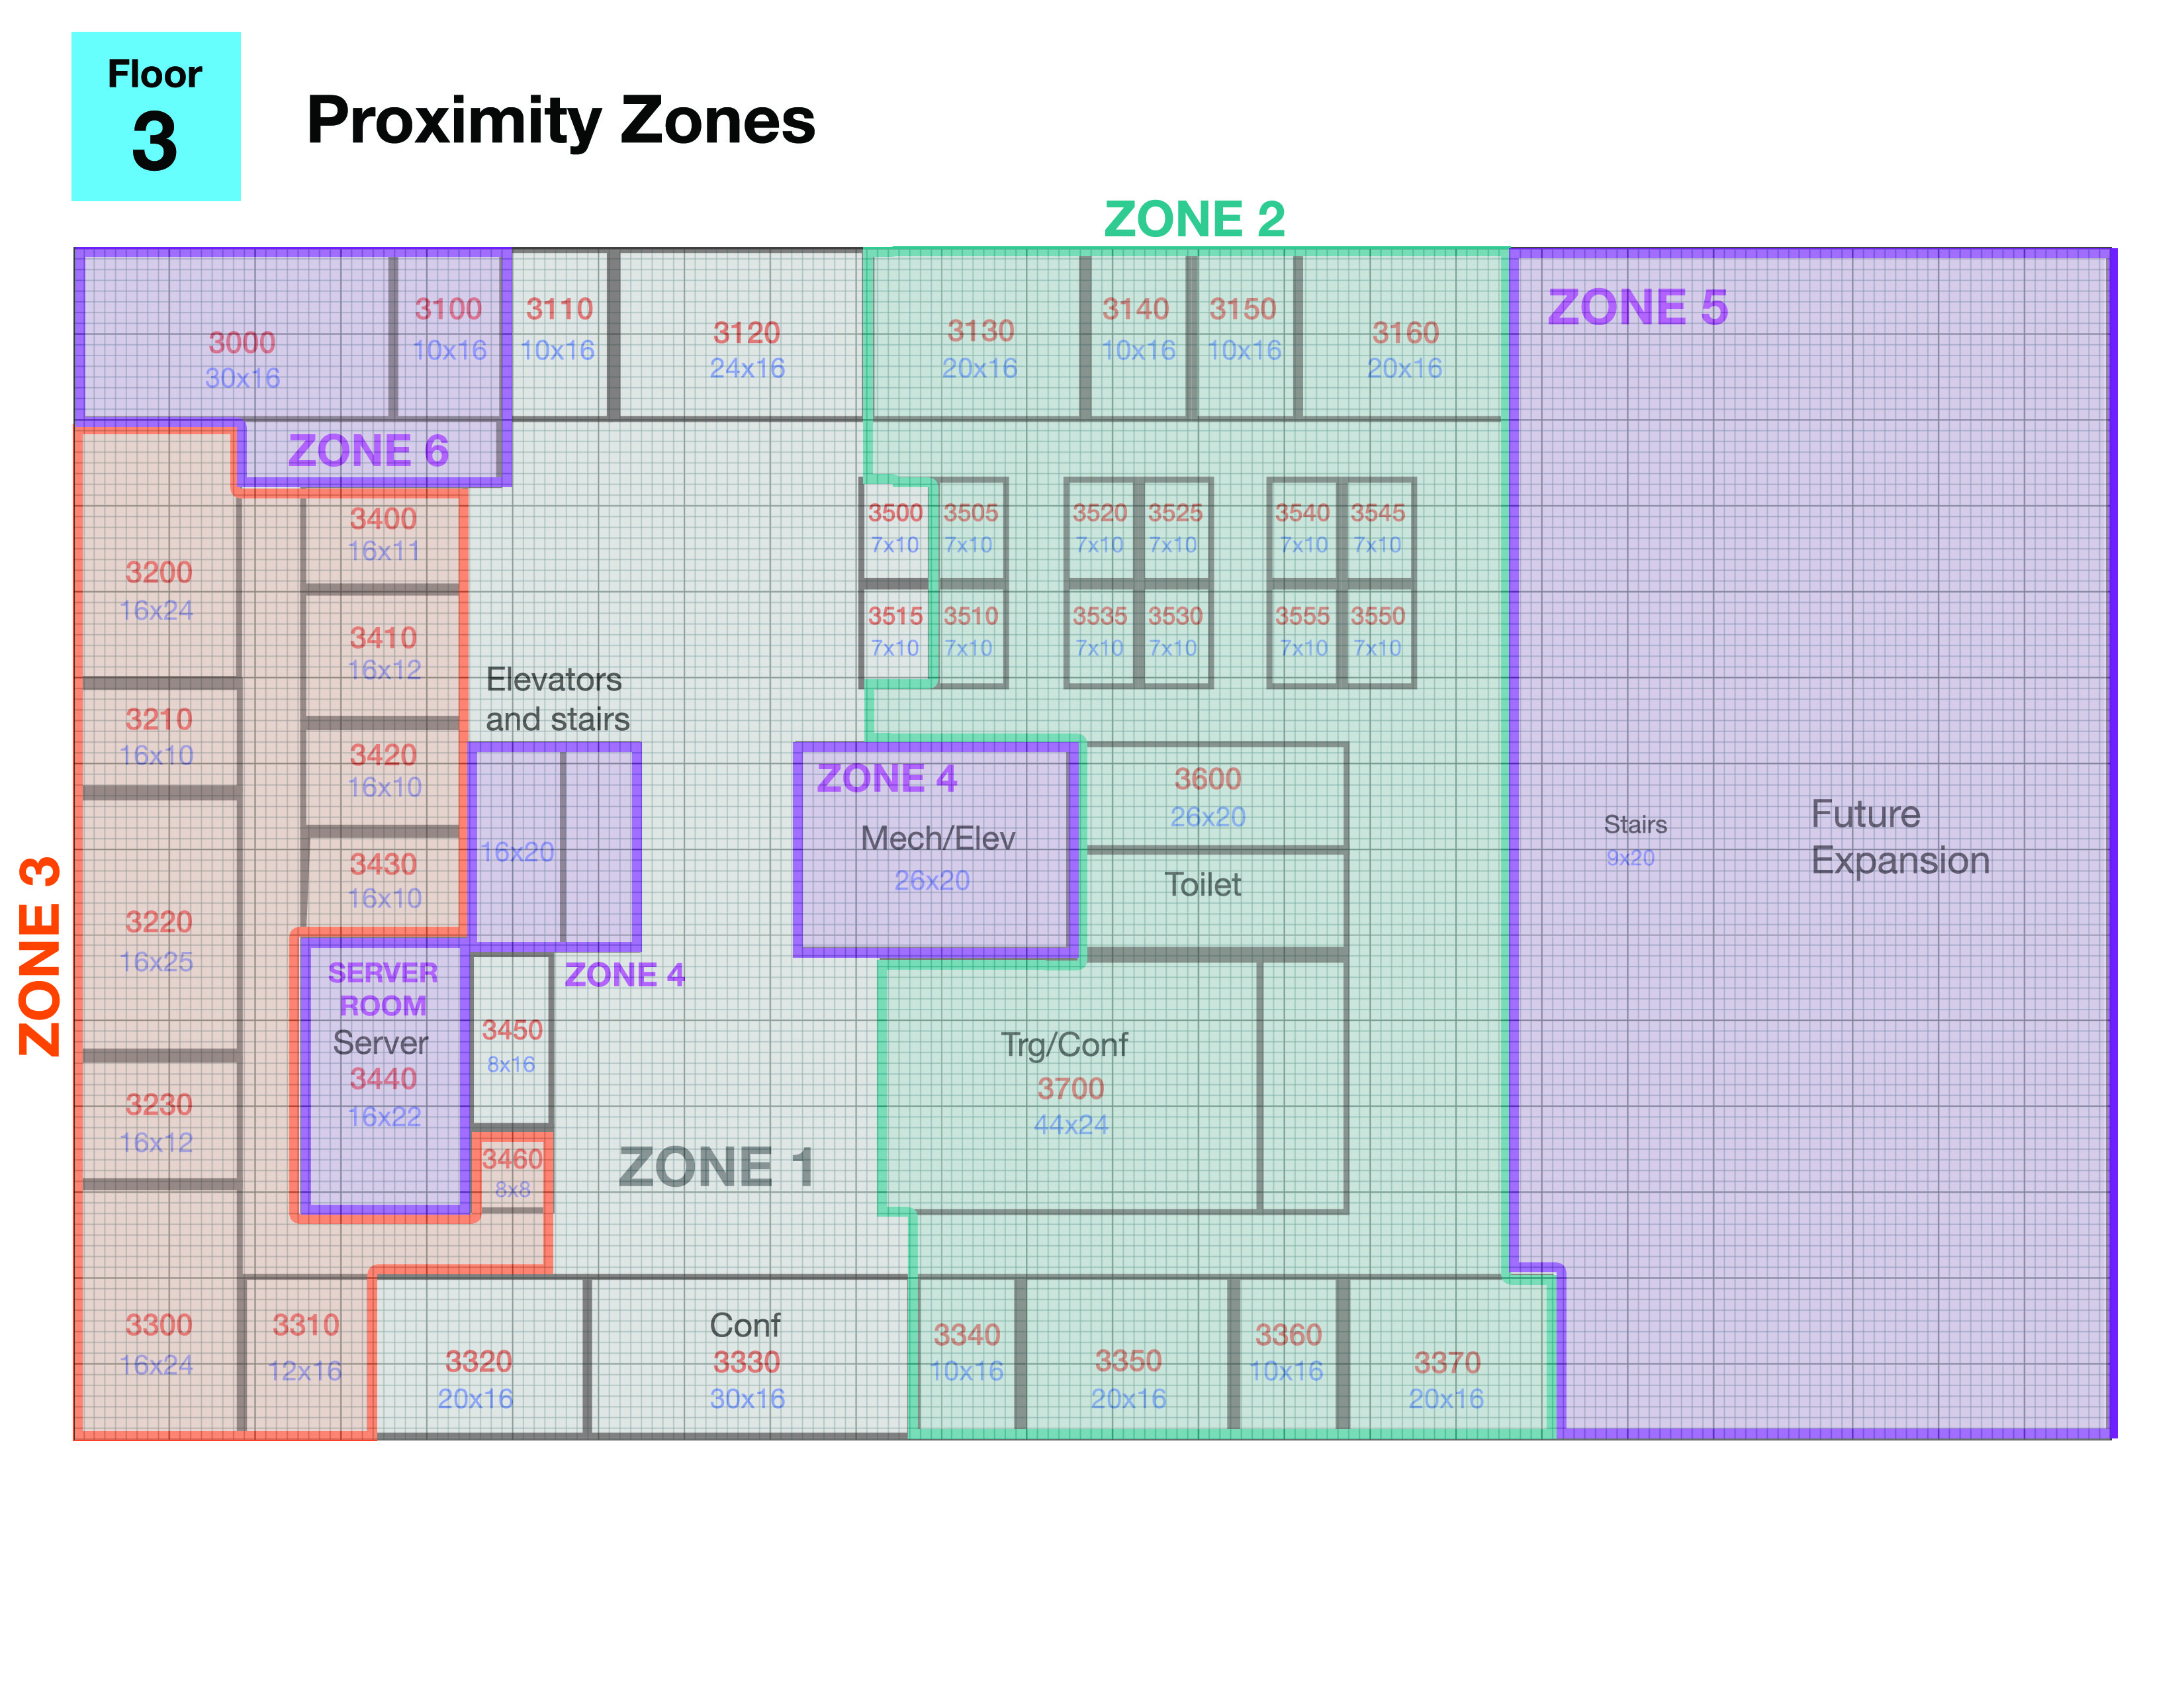
\includegraphics[width=0.3 \linewidth]{figures/prox3.jpg}
                        \\
                        
                        \mbox{(a) First Floor} & \mbox{(b) Second Floor} & \mbox{(c) Third Floor} \\
                    \end{array}$
                    \caption{Prox zone of the Building}
                    \label{fig:prox}
                \end{figure}
            
                The prox zone of this building is as figure \ref{fig:prox}.
    
    \section{Methods}
        \subsection{Python Packages}
            To analyze data, we used Python programming language. Also, we adopt many Python modules as hereinafter. 
        
            \subsubsection{Scikit-learn: Machine Learning in Python}
                \textit{Scikit-learn} is a Python module integrating a wide range of state-of-the-art machine learning algorithms for medium-scale supervised and unsupervised problems \cite{ref:sklearn1}.
                
            \subsubsection{Matplotlib}
                \textit{Matplotlib} is a Python 2D plotting library which produces publication quality figures in a variety of hardcopy formats and interactive environments across platforms \cite{ref:matplotlib1}.
                
            \subsubsection{Pandas}
                \textit{Pandas} is a Python library of rich data structures and tools for working with structured data sets common to statistic, finance, social sciences, and many other fields \cite{ref:pandas1}.
                
            \subsubsection{SciPy}
                \textit{SciPy} is a Python-based ecosystem of open-source software for mathematics, science, and engineering \cite{ref:scipy1}.
            
        \subsection{TSNE}
            T-distributed Stochastic Neighbor Embedding (TSNE) is a machine learning algorithm for visualization high-dimensional data in a low-dimensional space \cite{ref:tsne1}.
    
    \section{Results}
        \subsection[Question 1]{What are the typical patterns in the prox card data? What does a typical day look like for GAStech employees?}
            \subsubsection{General Information of prox Data}
                First of all, we drew the distribution of movement distance as figure \ref{fig:movementdist}. Also, the basic statistics values, such as minimum, maximum, and average, of movement distance is in table \ref{tb:movementdist}.
            
                \begin{figure}[htbp]
                    \centering
                    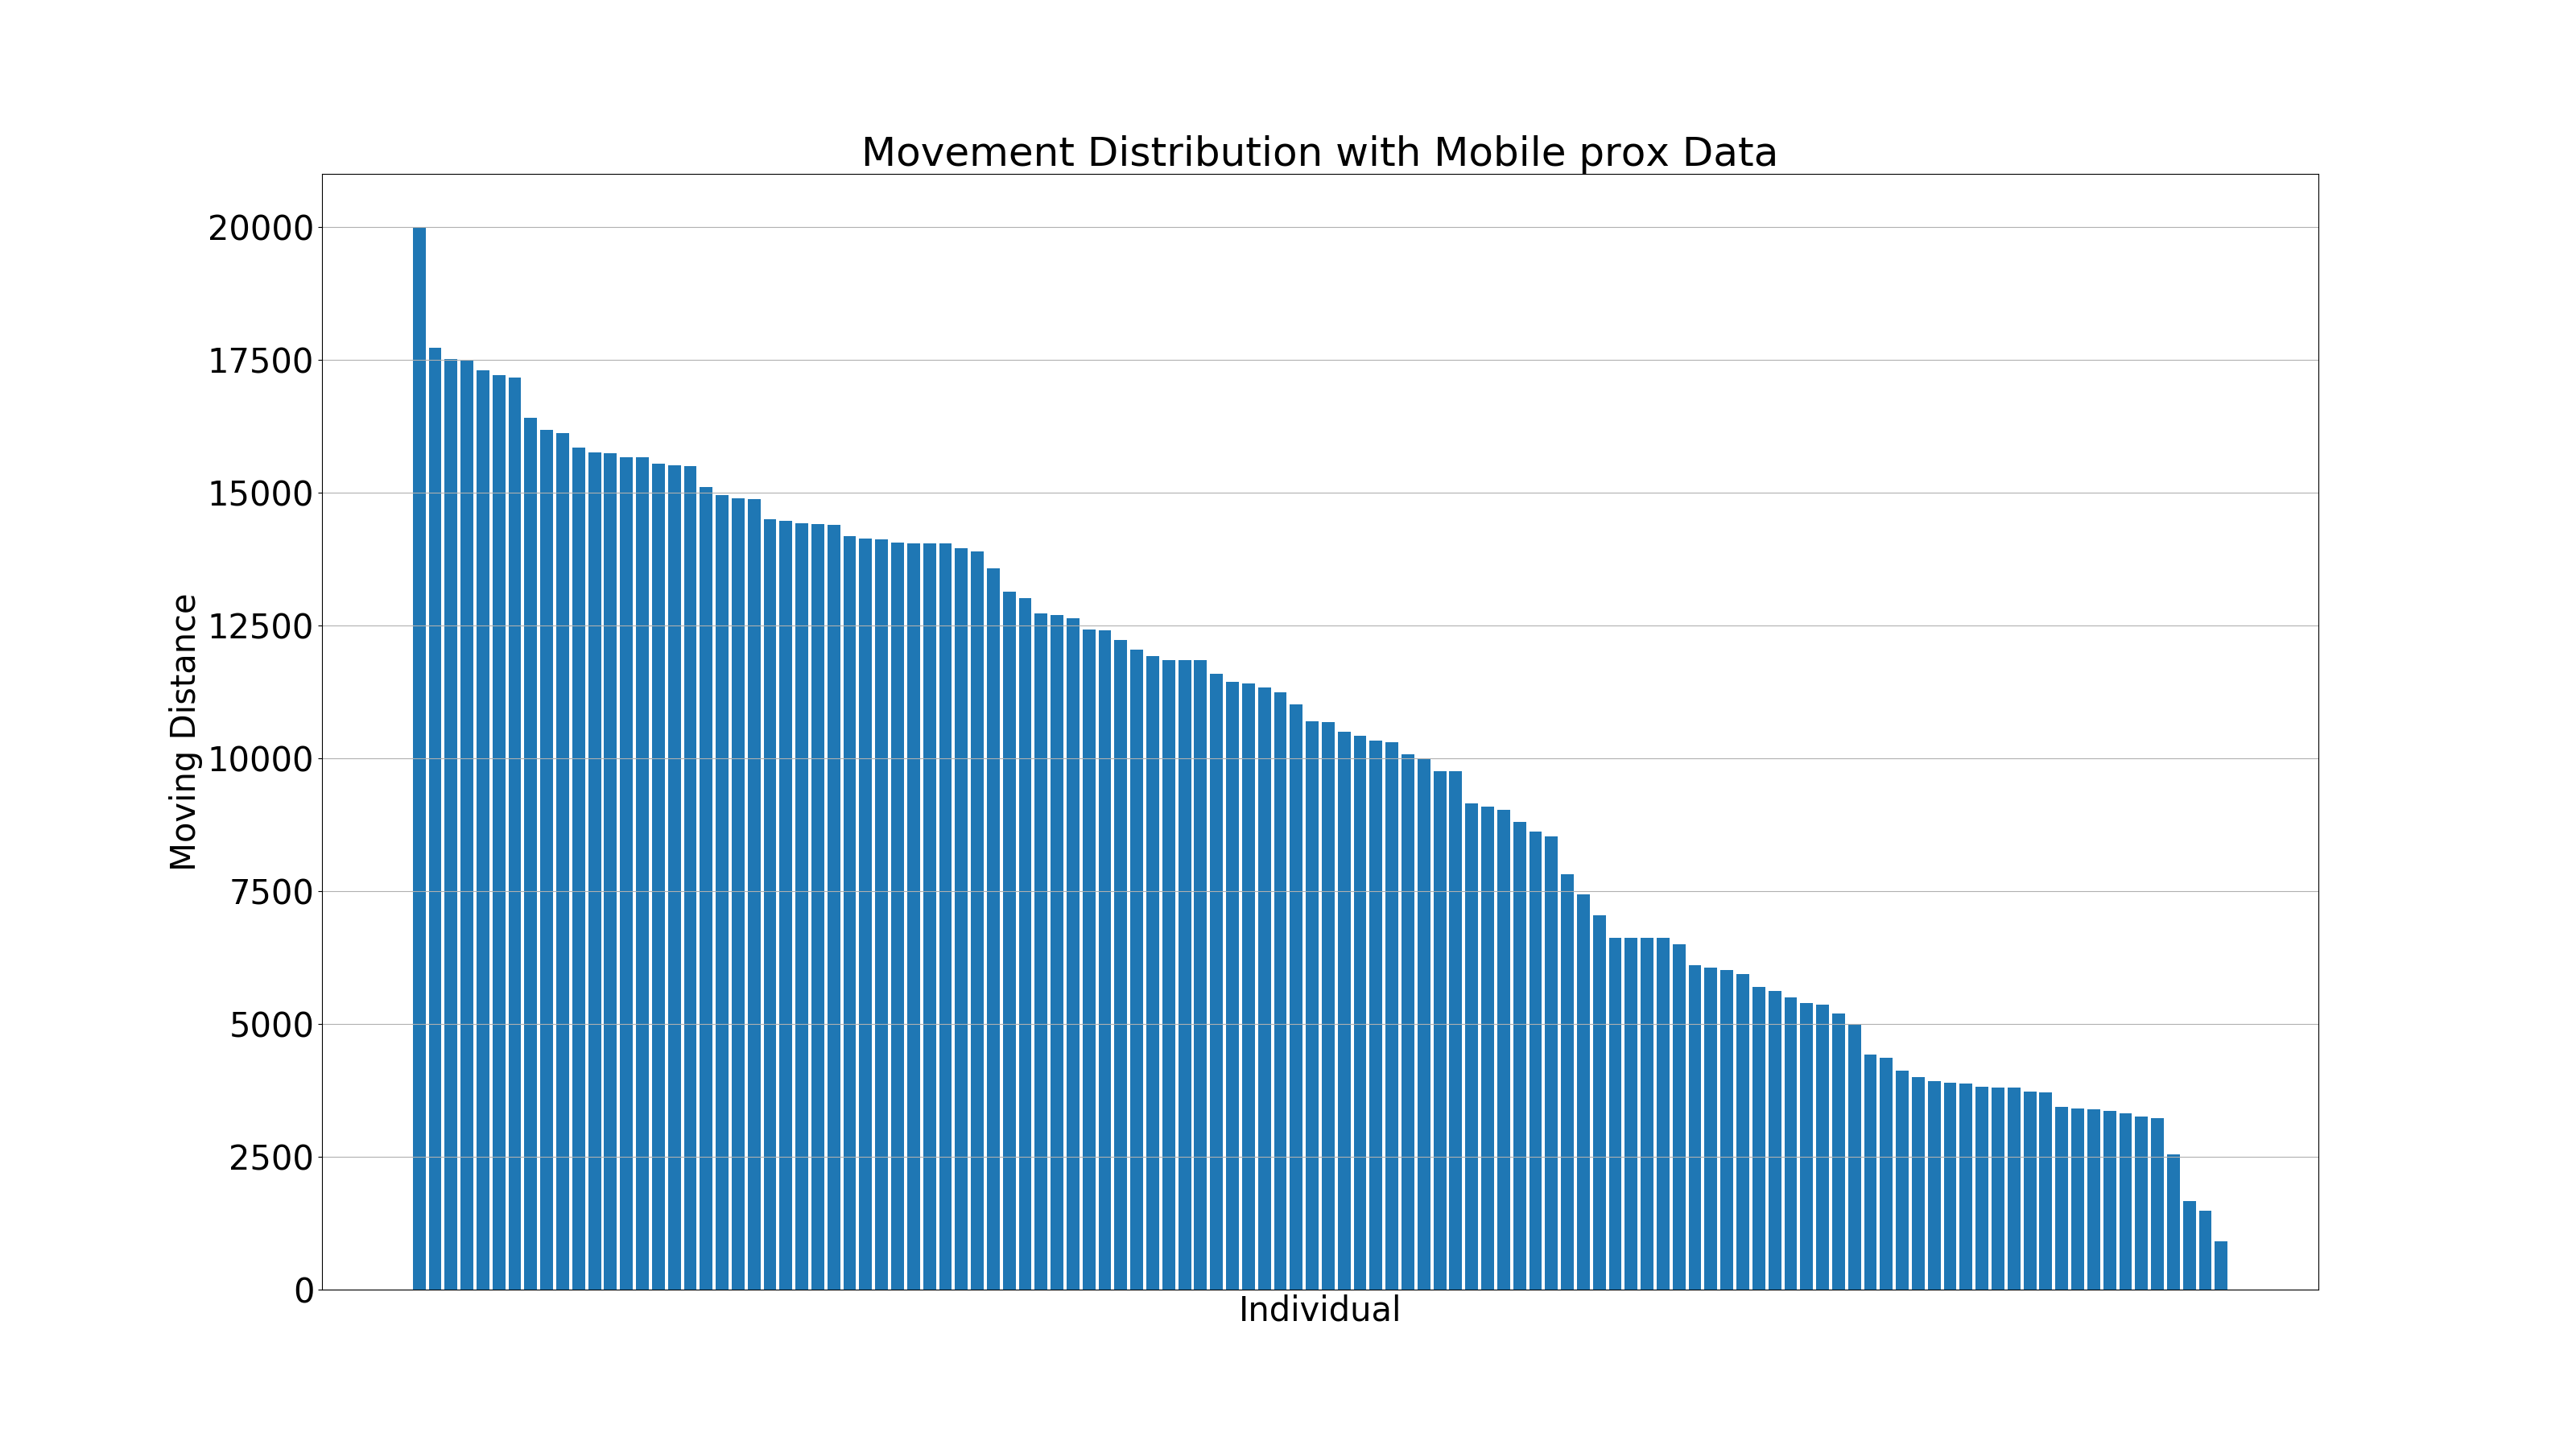
\includegraphics[width=0.6 \linewidth]{figures/movementdistribution.png}
                    \caption{Distribution of Movement Distance}
                    \label{fig:movementdist}
                \end{figure}
        
                \begin{table}[htbp]
                    \centering
                    \caption{Basic Statistics Data within Movement Distance}
                    \label{tb:movementdist}
                    \begin{tabular}{c||c|c|c|c|c|c|c}
                        Item & Minimum & Maximum & Average & q1 & Median & q3 & Standard Deviation \\ \hline
                        Value & 902.44 & 19999.38 & 10083.95 & 5642.54 & 10688.57 & 14134.16 & 4750.46 \\
                    \end{tabular}
                \end{table}
            
            \subsubsection{Workflow}
                With the general information of prox data, we have decided our workflow for question 1 as figure \ref{fig:workflow1}.
                
                \begin{figure}[htbp]
                    \centering
                    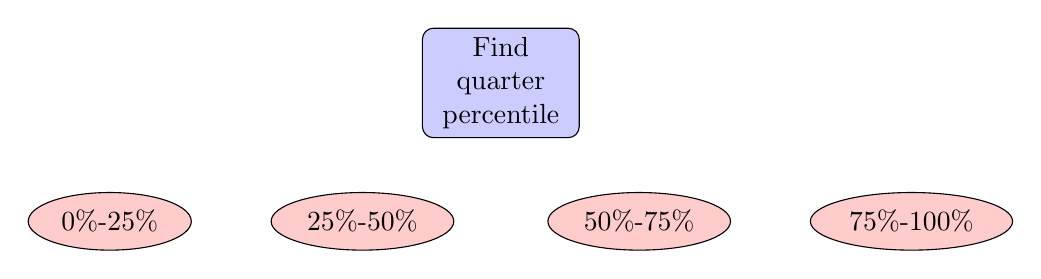
\begin{tikzpicture}[node distance = 2cm, auto]
                        \node[block](root1){Find quarter percentile};
                        \node[cloud, below of=root1, left of=root1](q2){25\%-50\%};
                        \node[cloud, below of=root1, right of=root1](q3){50\%-75\%};
                        \node[cloud, left=1cm of q2](q1){0\%-25\%};
                        \node[cloud, right=1cm of q3](q4){75\%-100\%};
                    \end{tikzpicture}
                    \caption{Workflow for Question 1}
                    \label{fig:workflow1}
                \end{figure}
        
            \subsubsection{Movement Direction and Distance}
                We drew the plot about movement direction and distance with each sub-group as figures \ref{fig:movedd1}, \ref{fig:movedd2}, and \ref{fig:movedd3}. Note that the darkness of arrow is proportioned with number of duplicates. 
            
                \begin{figure}[htbp]
                    \centering
                    $\begin{array}{cc}
                        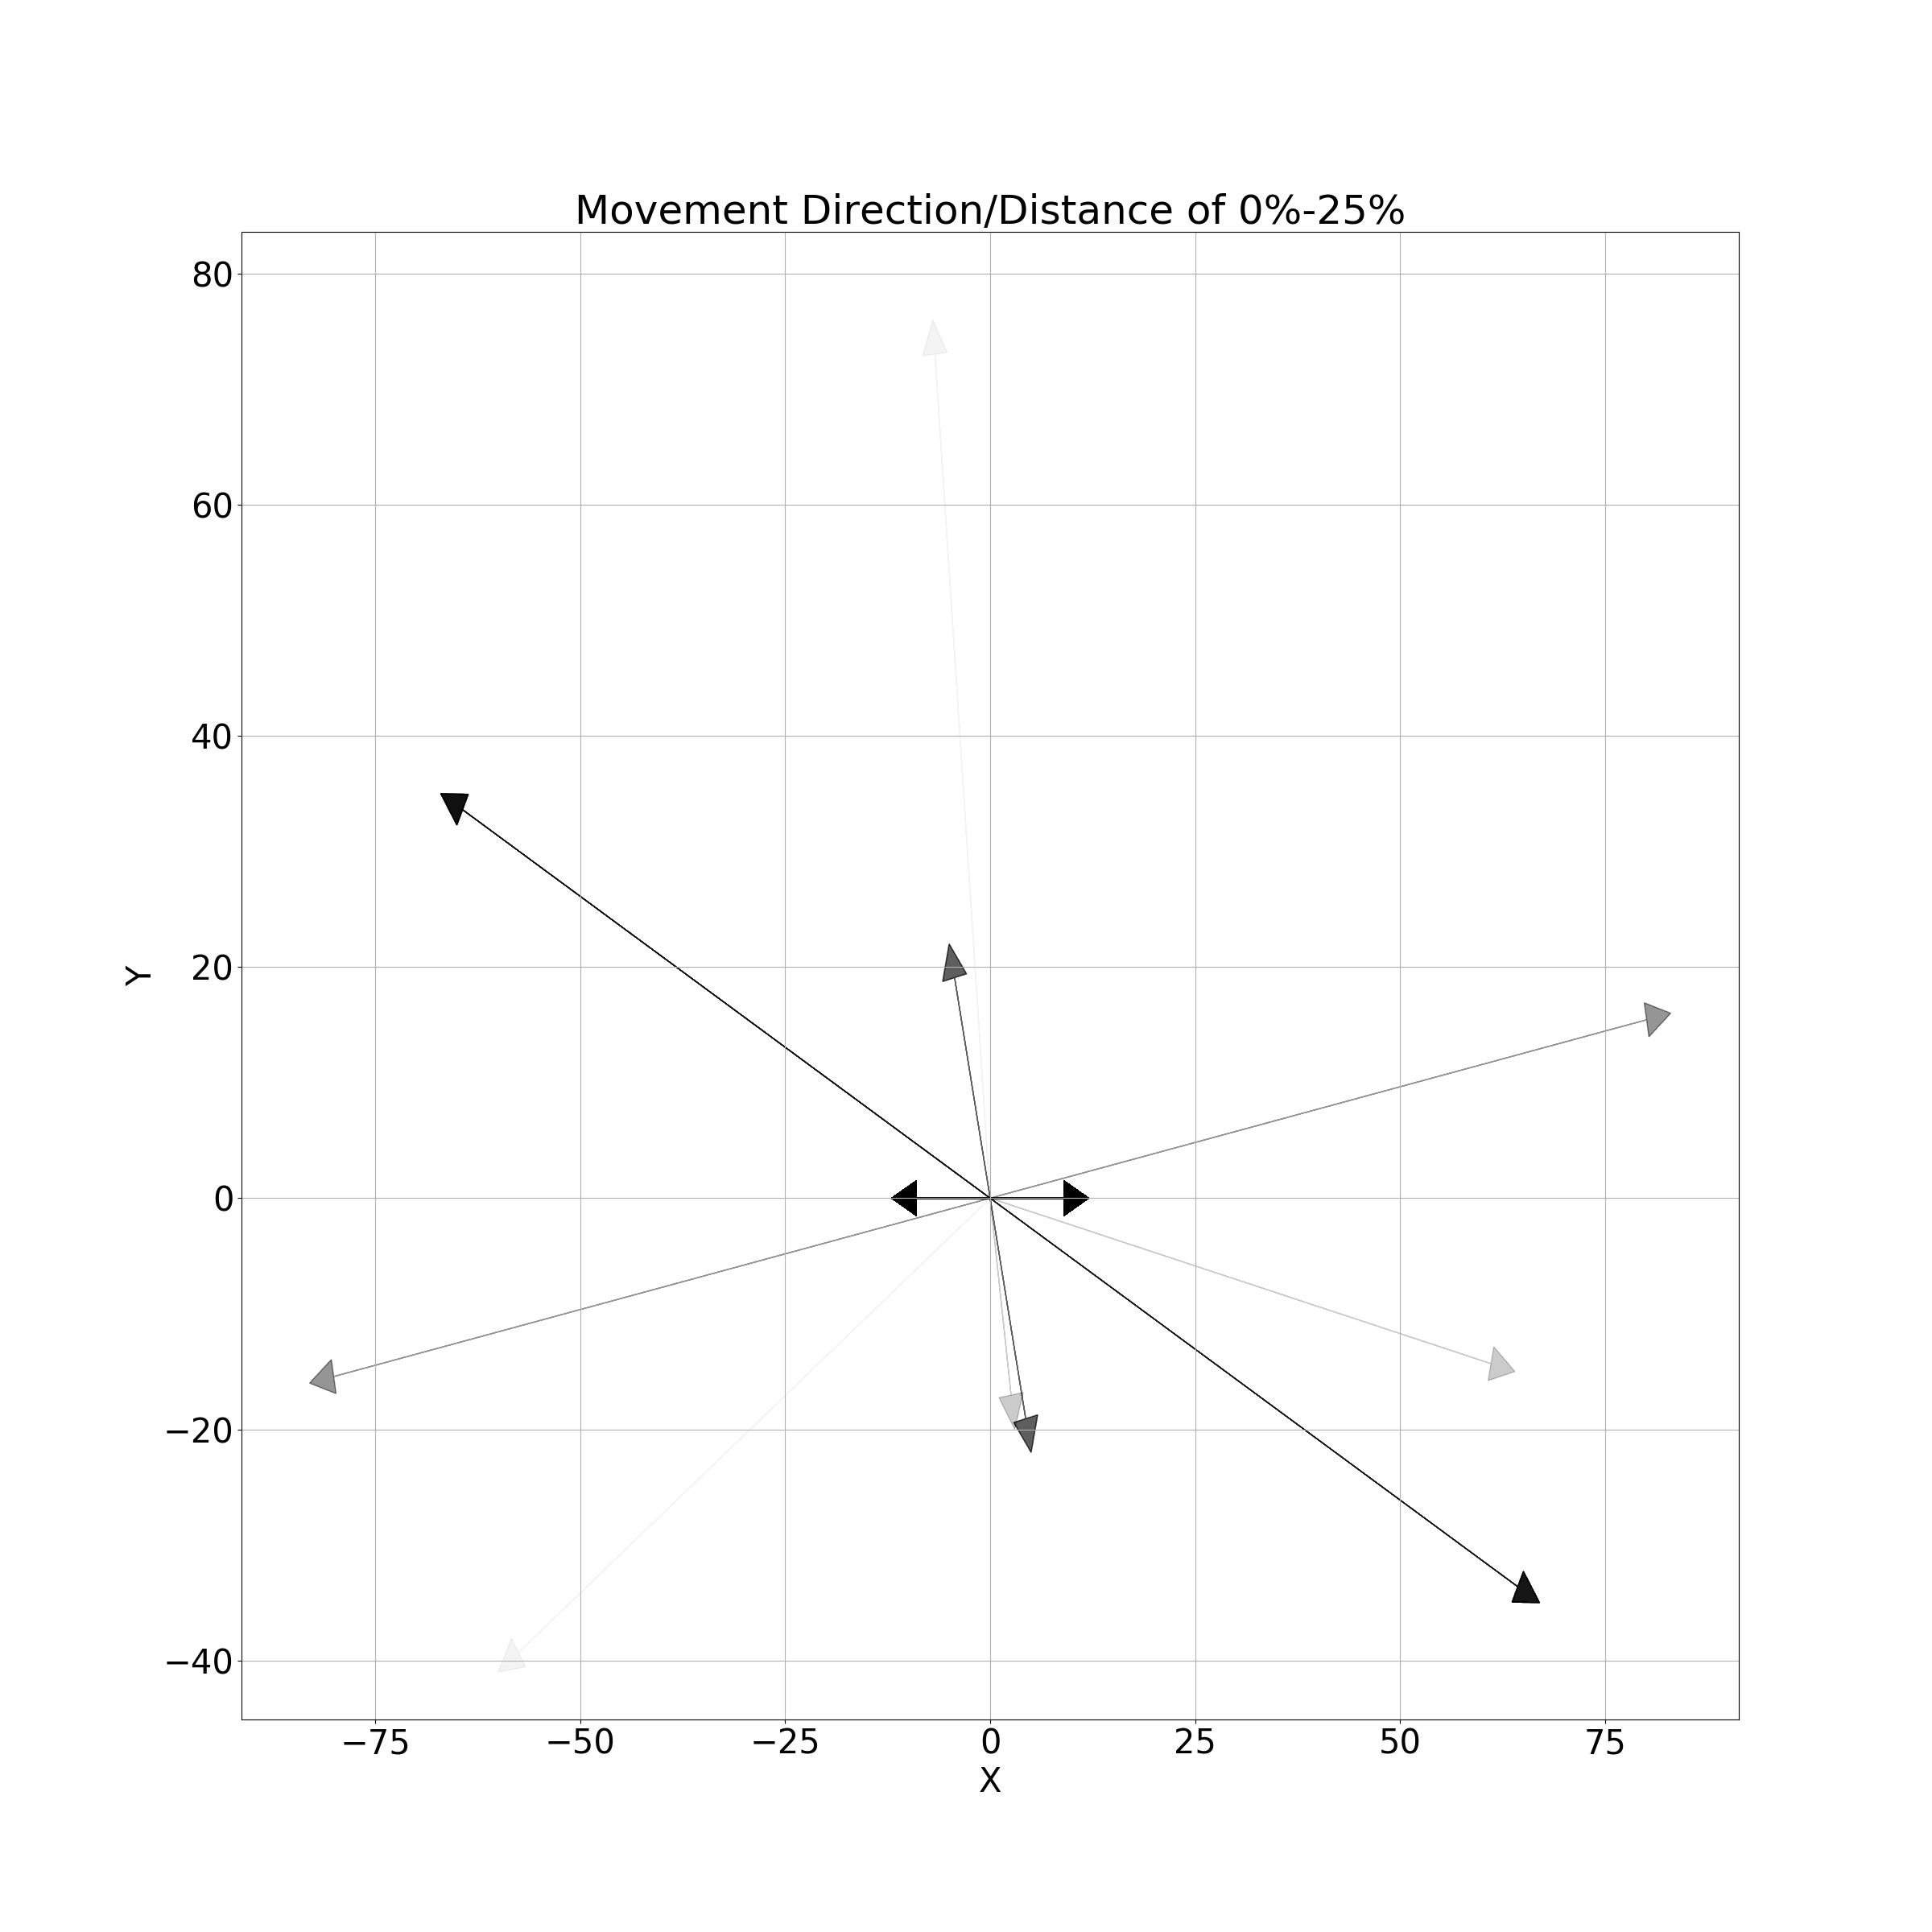
\includegraphics[width=0.3 \linewidth]{figures/movement1-1.png}
                        &
                        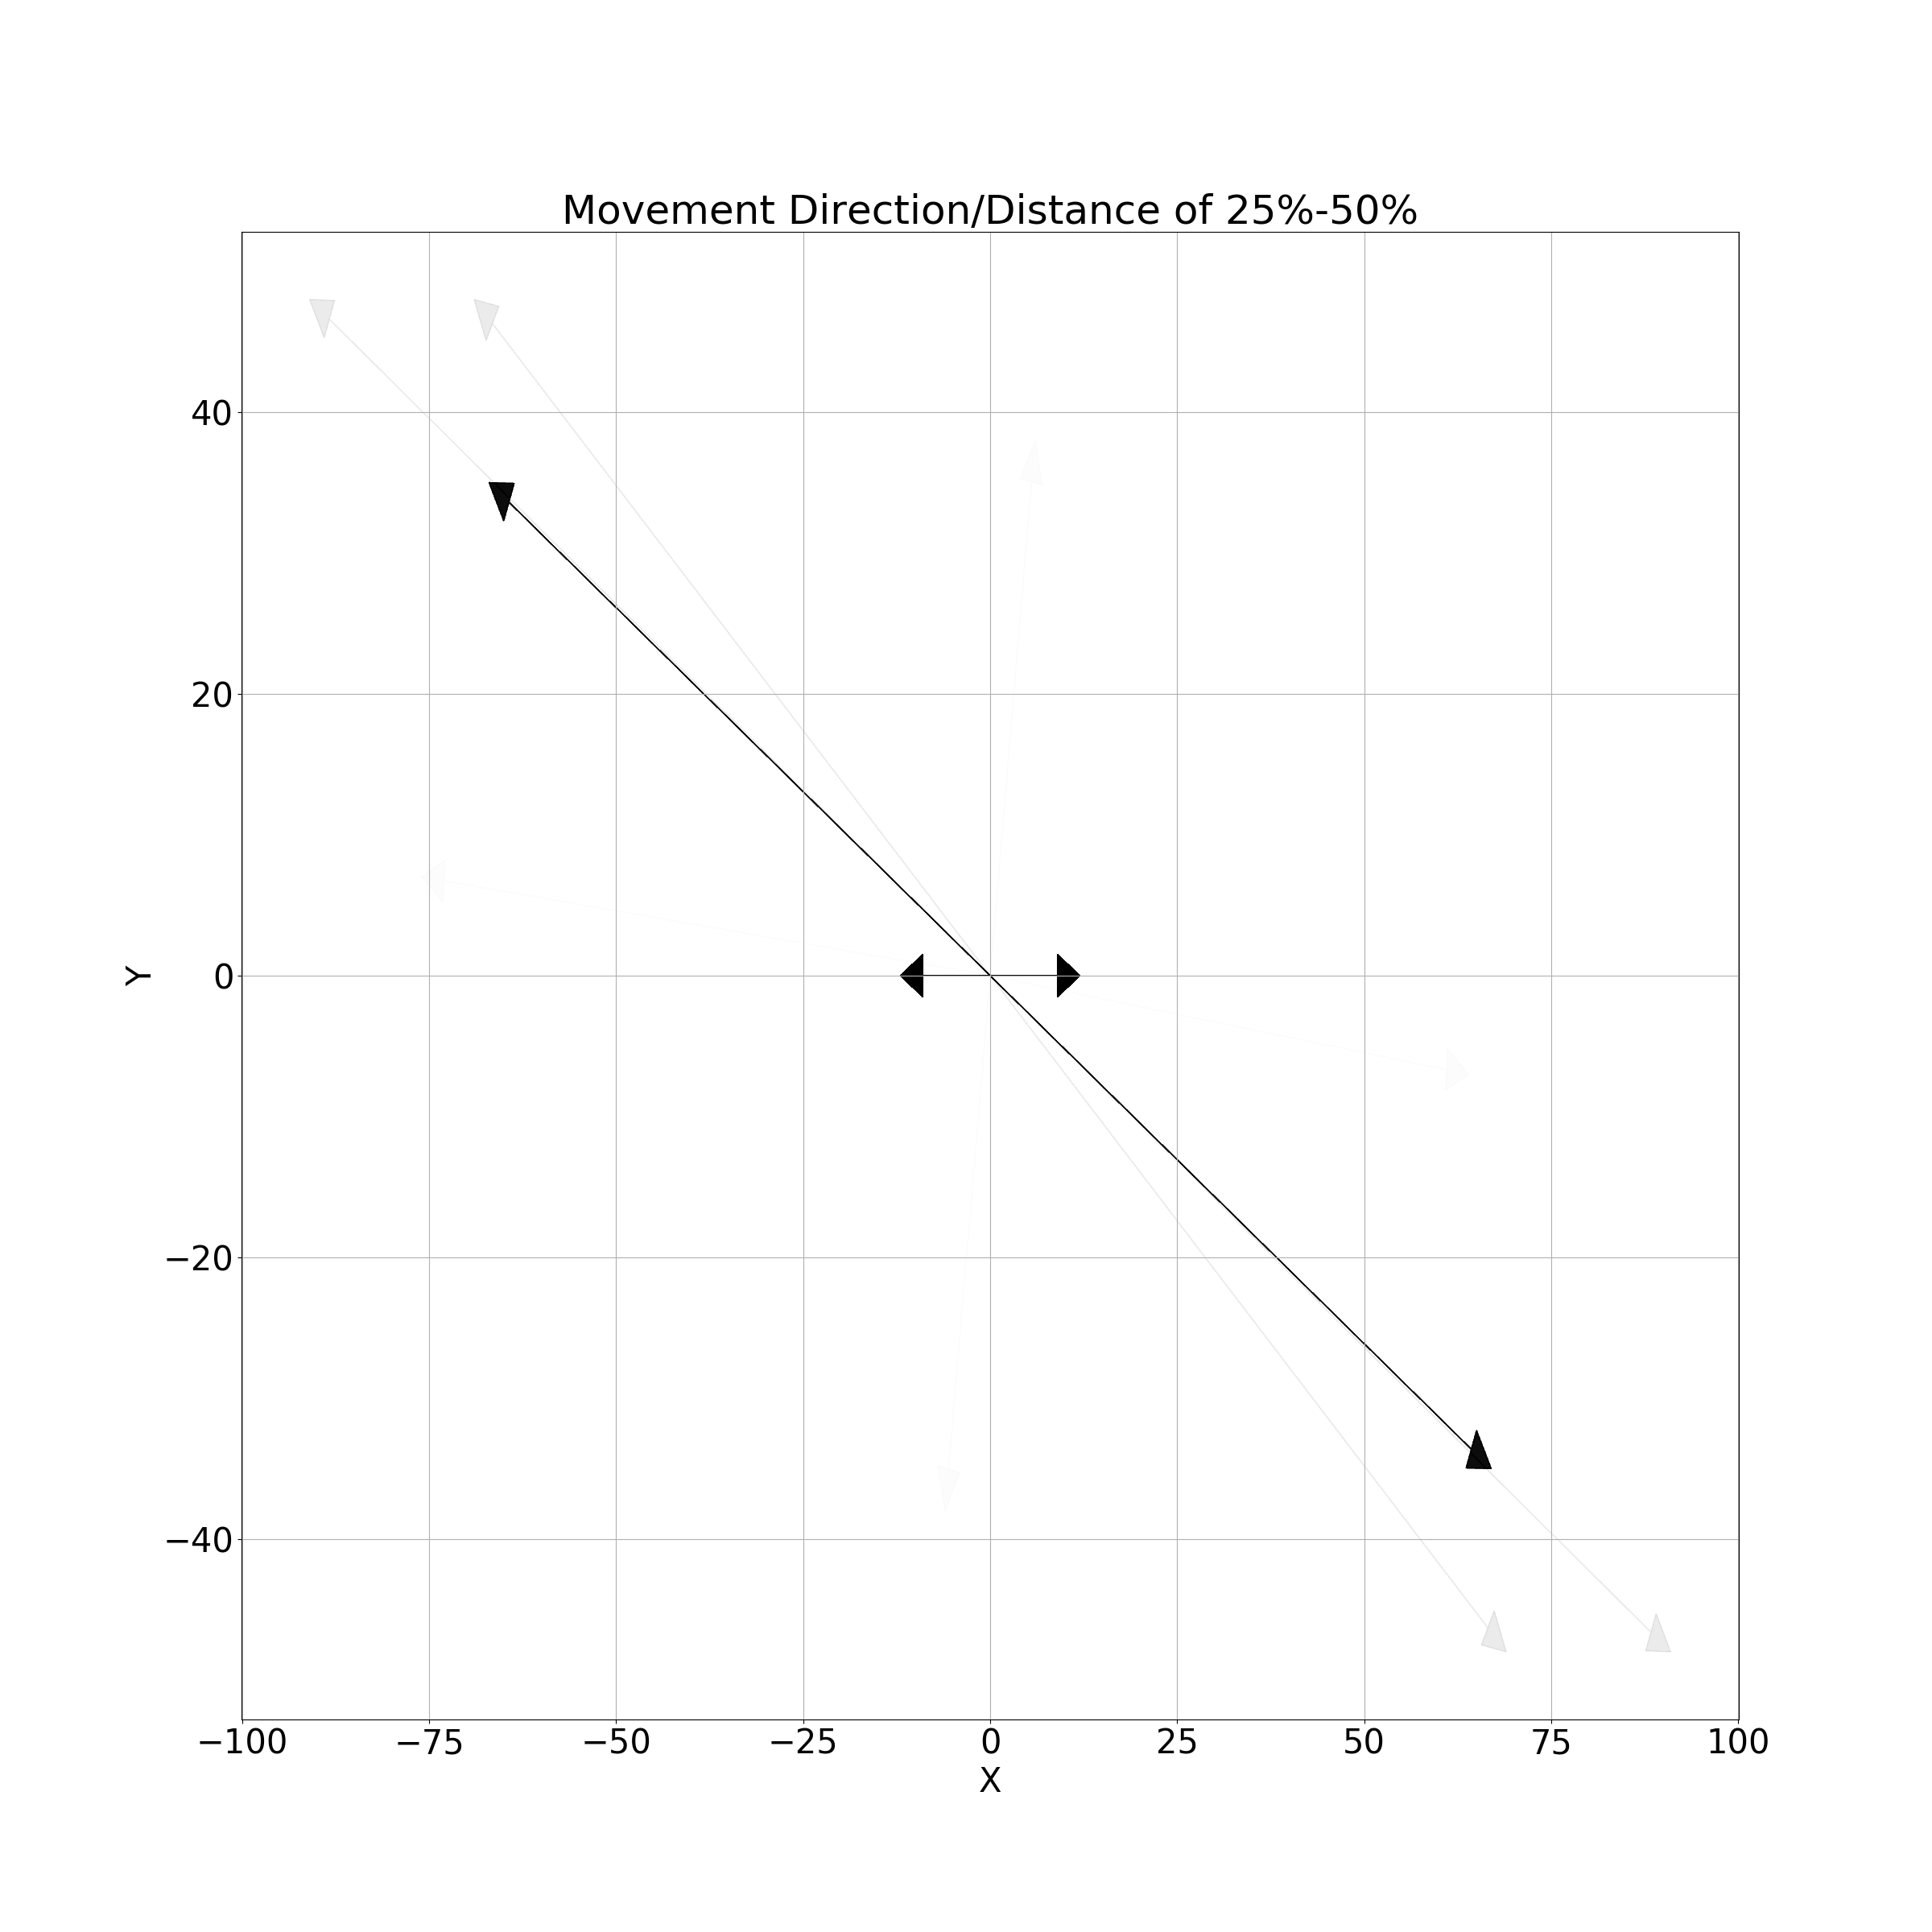
\includegraphics[width=0.3 \linewidth]{figures/movement1-2.png}
                        \\
                        
                        \mbox{(a) 0\%-25\%} & \mbox{(b) 25\%-50\%} \\
                        
                        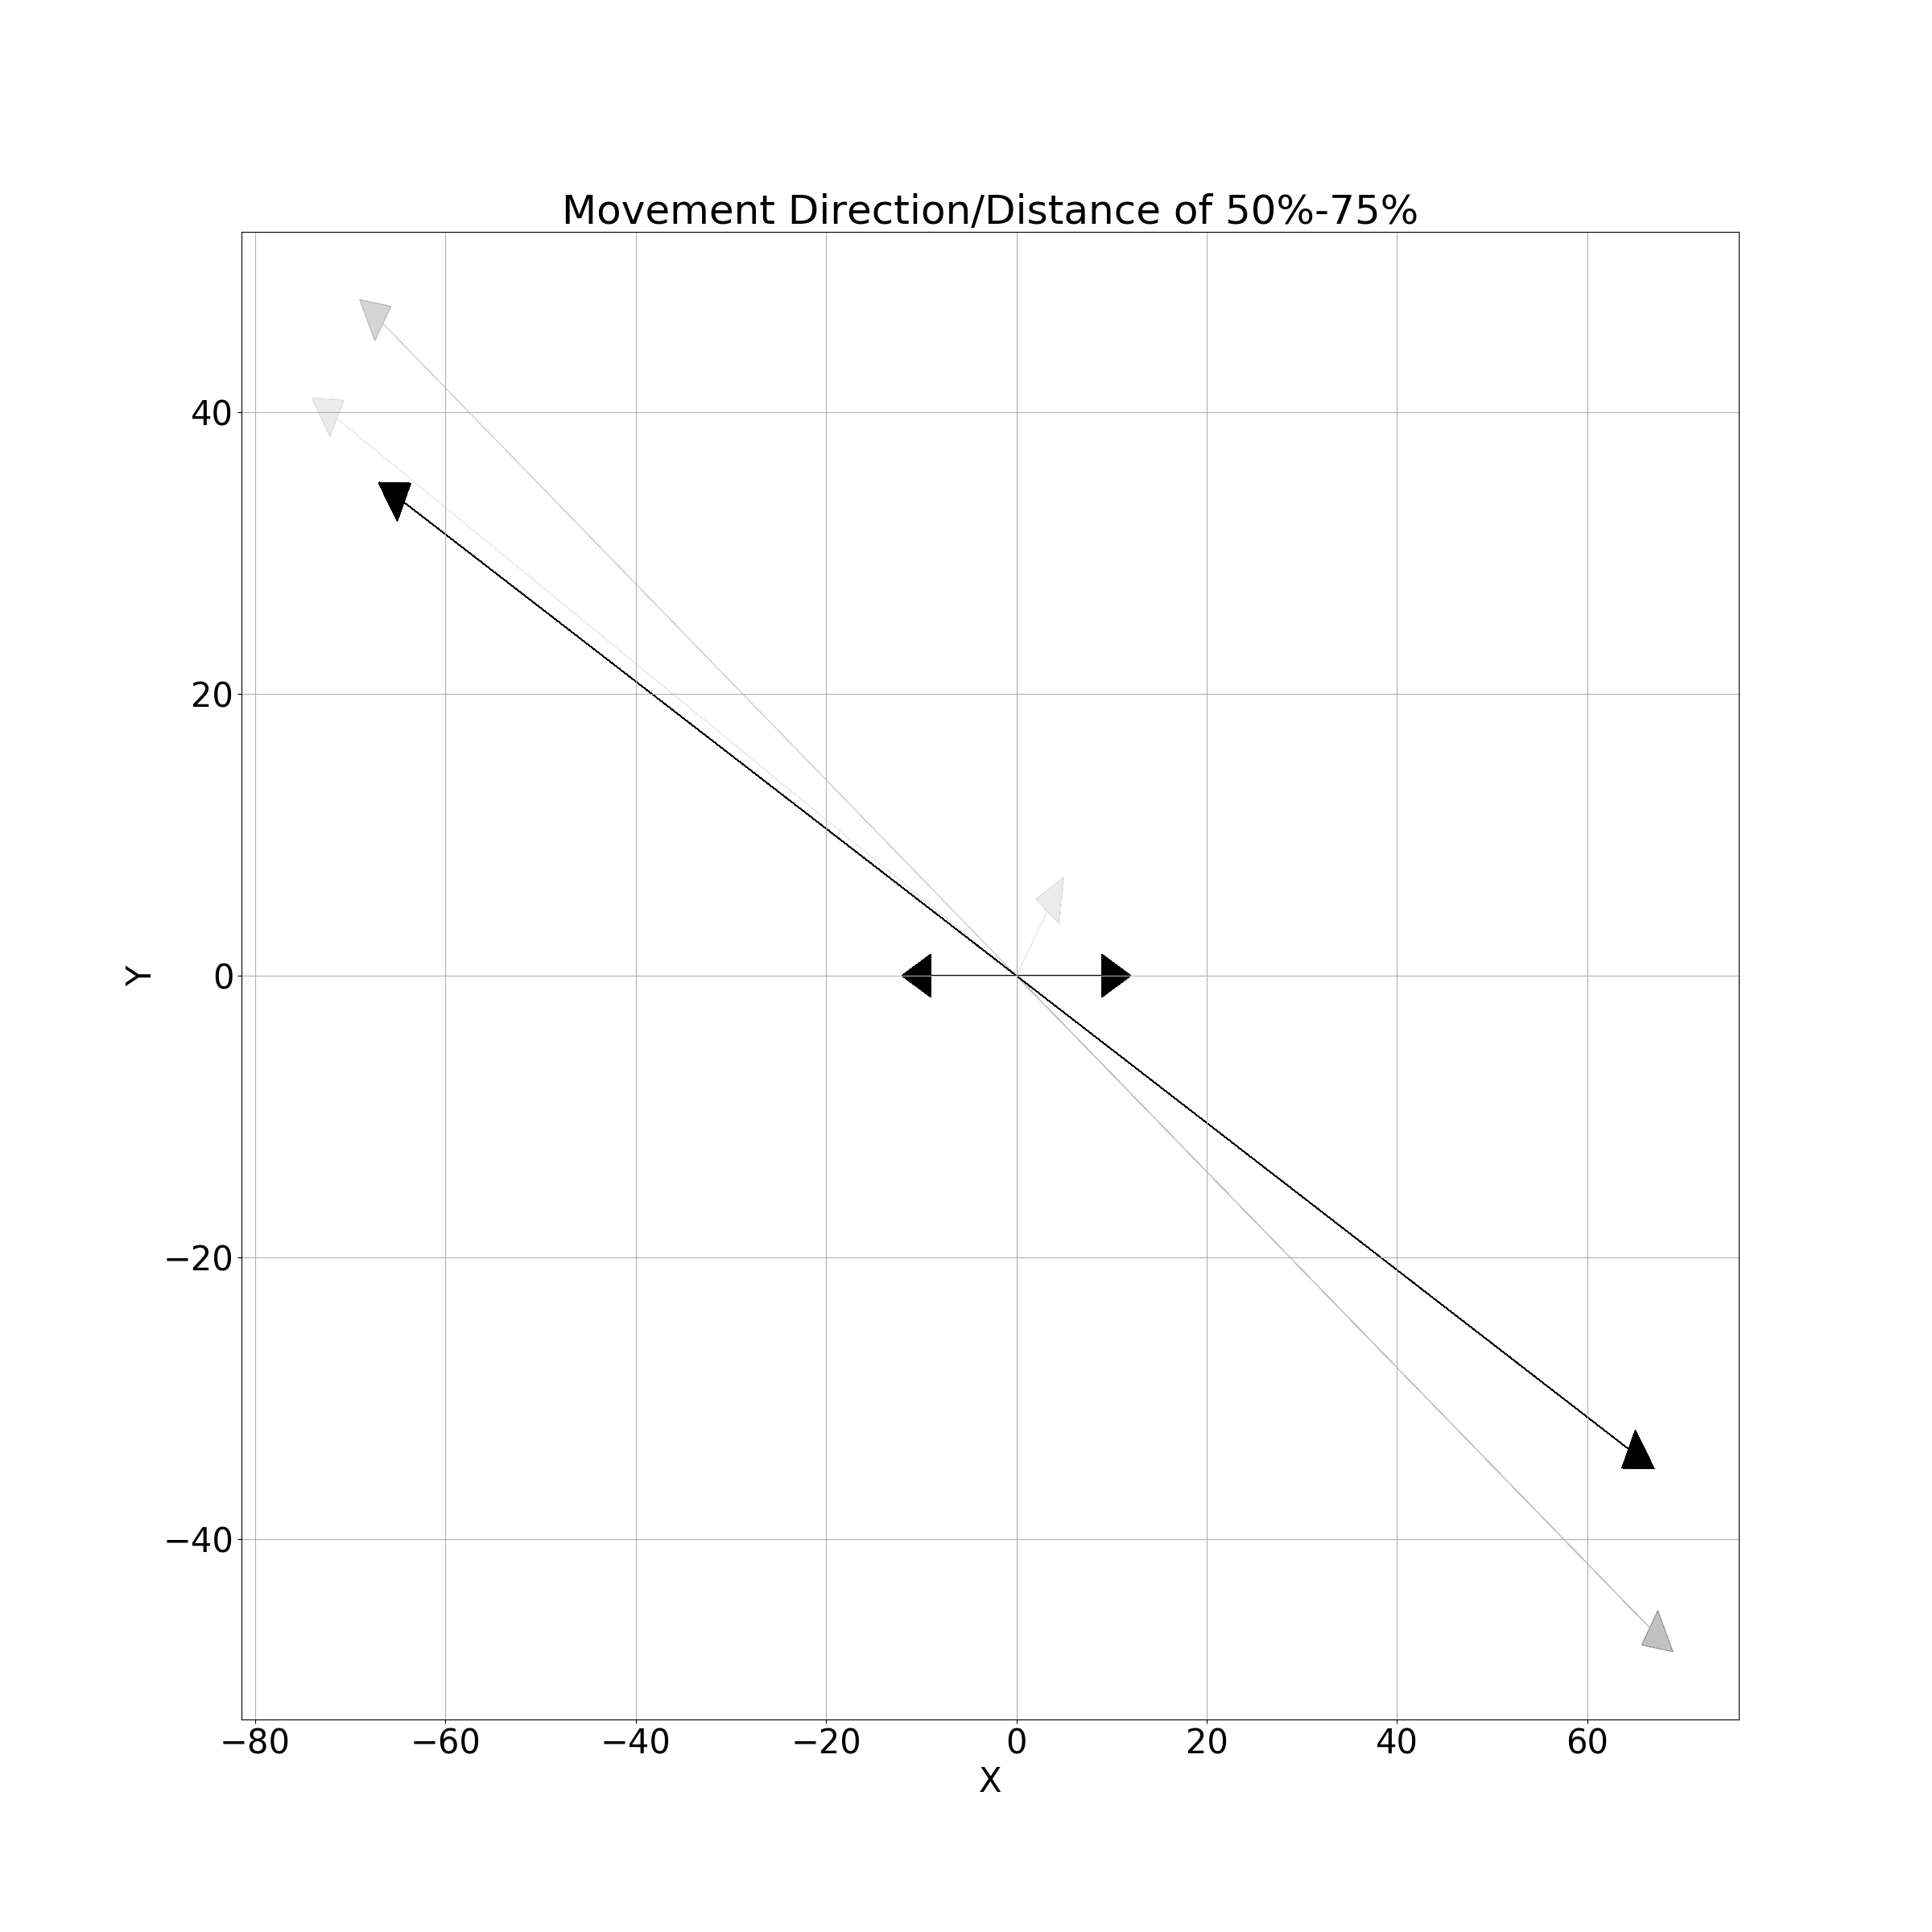
\includegraphics[width=0.3 \linewidth]{figures/movement1-3.png}
                        &
                        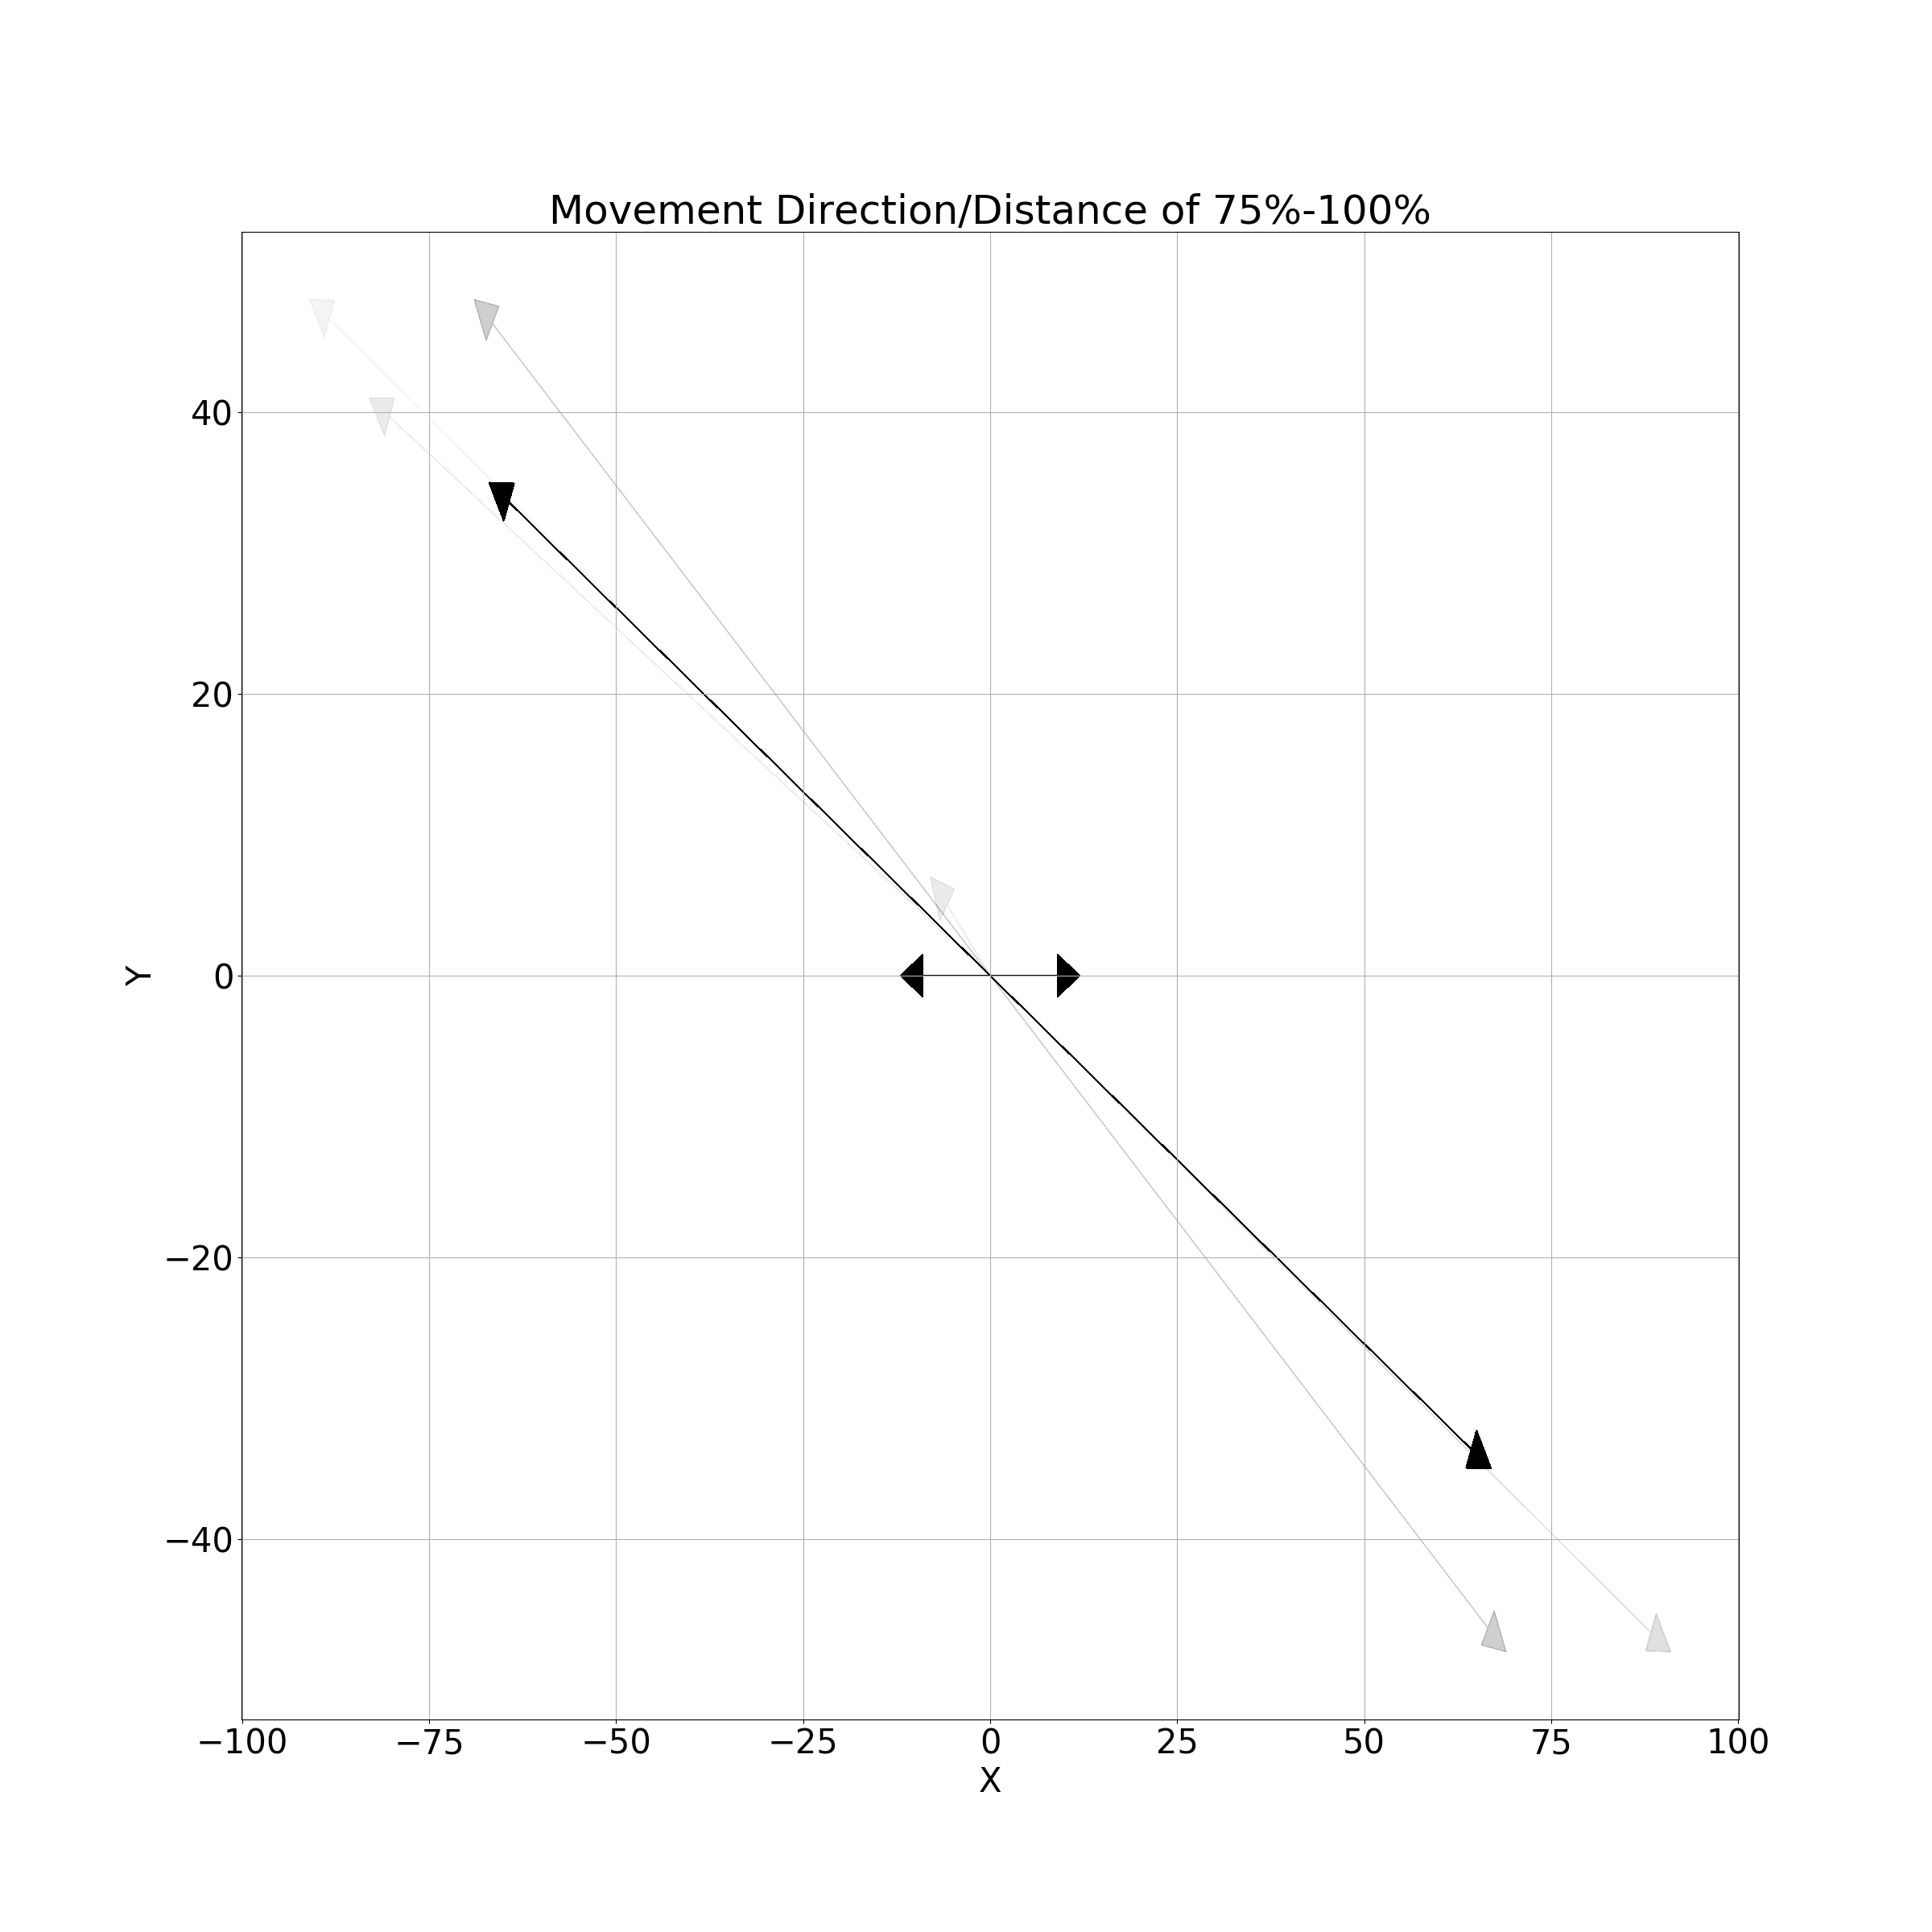
\includegraphics[width=0.3 \linewidth]{figures/movement1-4.png}
                        \\
                        
                        \mbox{(c) 50\%-75\%} & \mbox{(d) 75\%-100\%} \\
                    \end{array}$
                    \caption{Movement Direction/Distance on First Floor}
                    \label{fig:movedd1}
                \end{figure}
            
                The movement direction and distance on the first floor is shows as figure \ref{fig:movedd1}. In figure \ref{fig:movedd1}-(b, c, d), you can see two arrows: one is left-upward arrow, the other is right-downward arrow. 
                
                \begin{figure}[htbp]
                    \centering
                    $\begin{array}{cc}
                    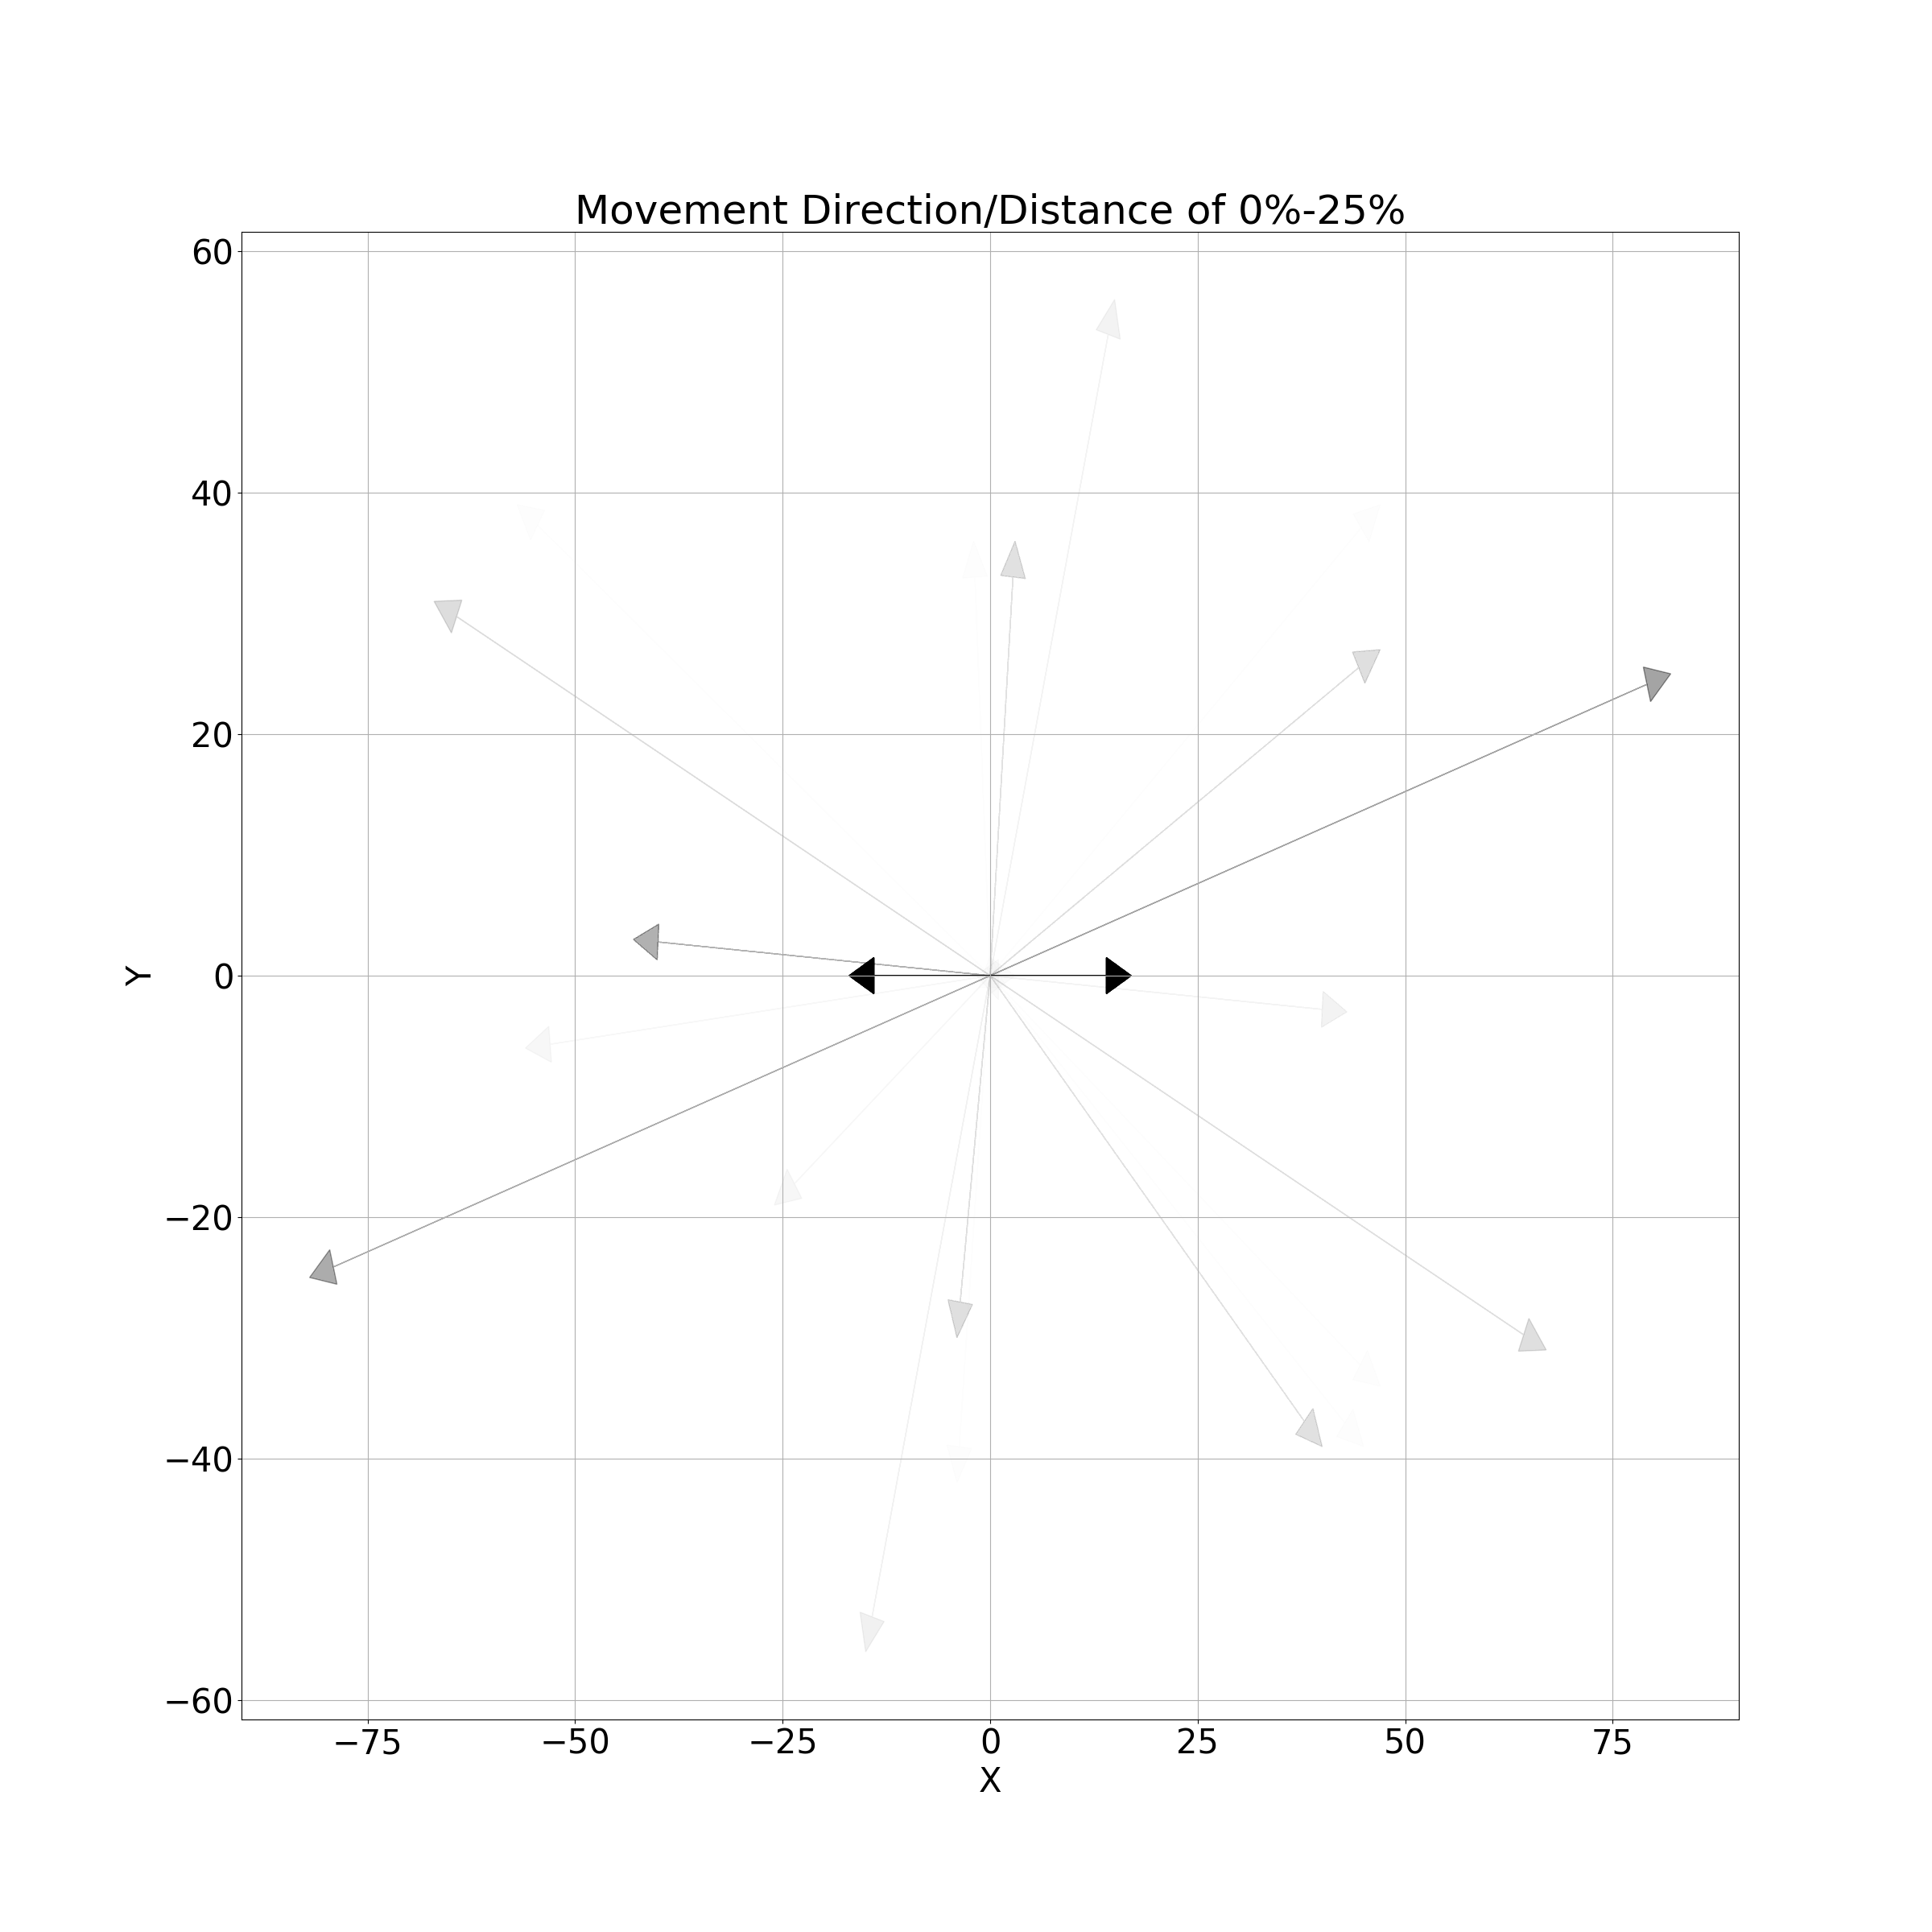
\includegraphics[width=0.3 \linewidth]{figures/movement2-1.png}
                    &
                    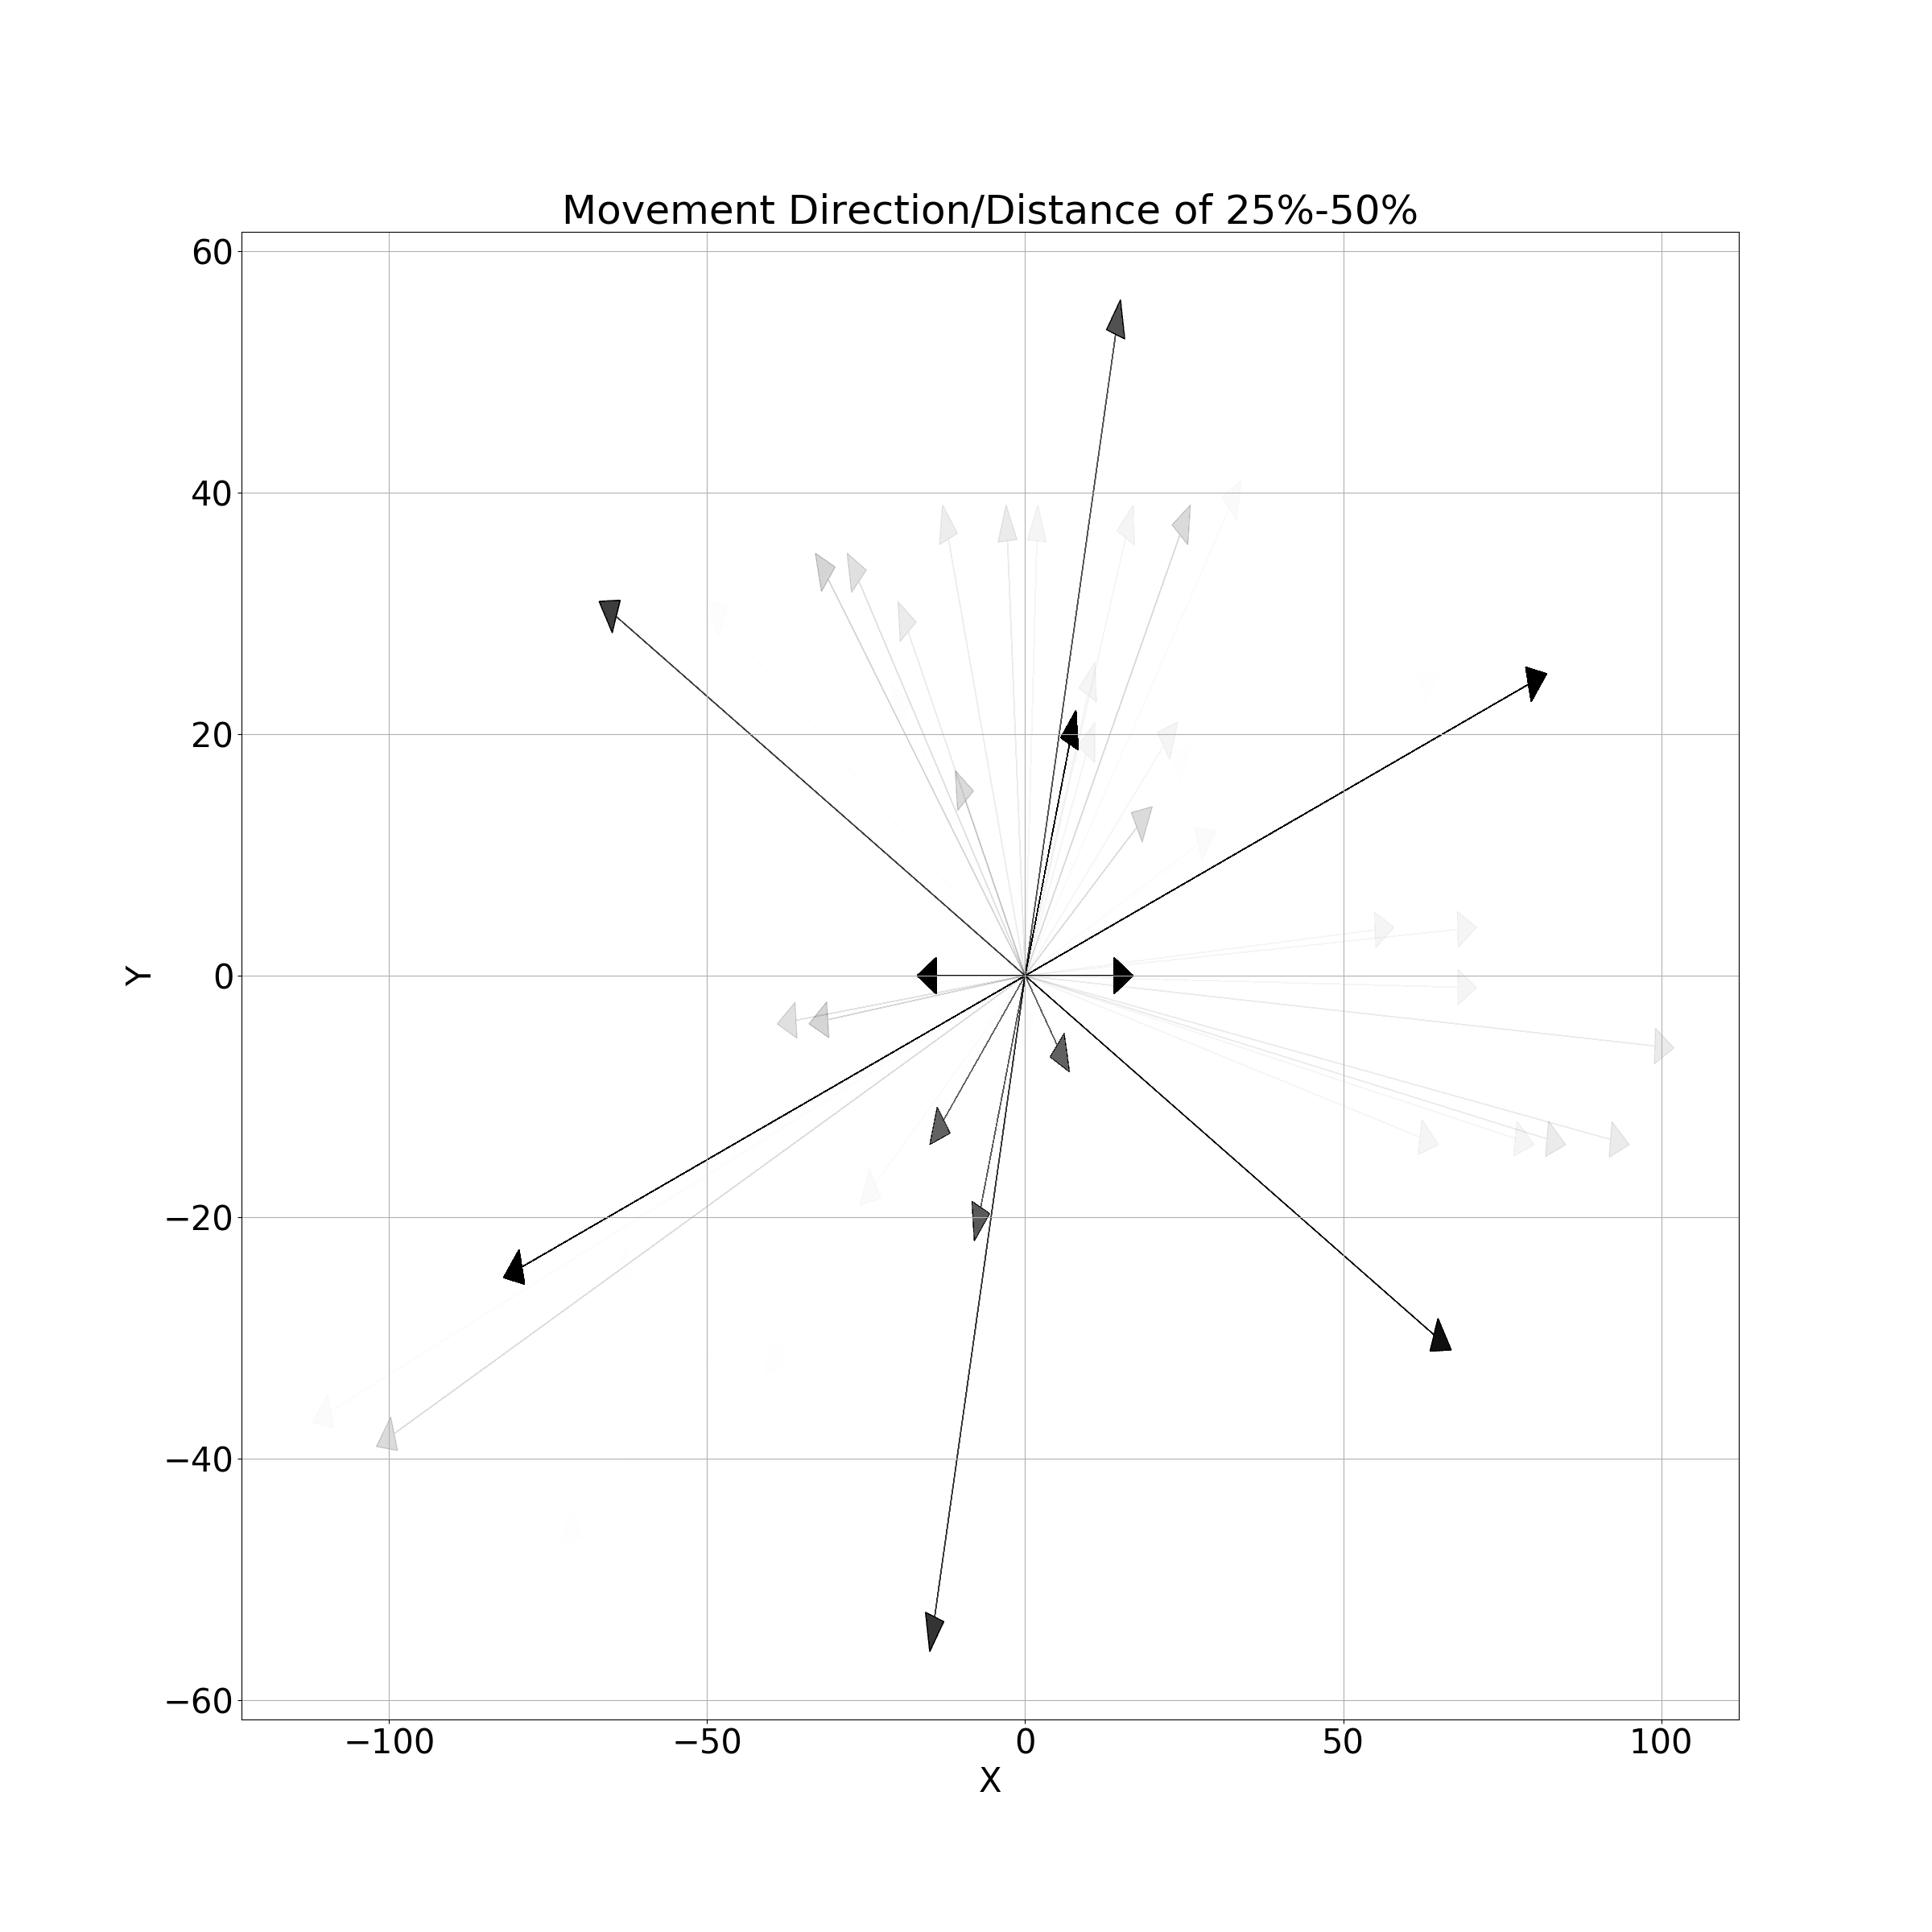
\includegraphics[width=0.3 \linewidth]{figures/movement2-2.png}
                    \\
                    
                    \mbox{(a) 0\%-25\%} & \mbox{(b) 25\%-50\%} \\
                    
                    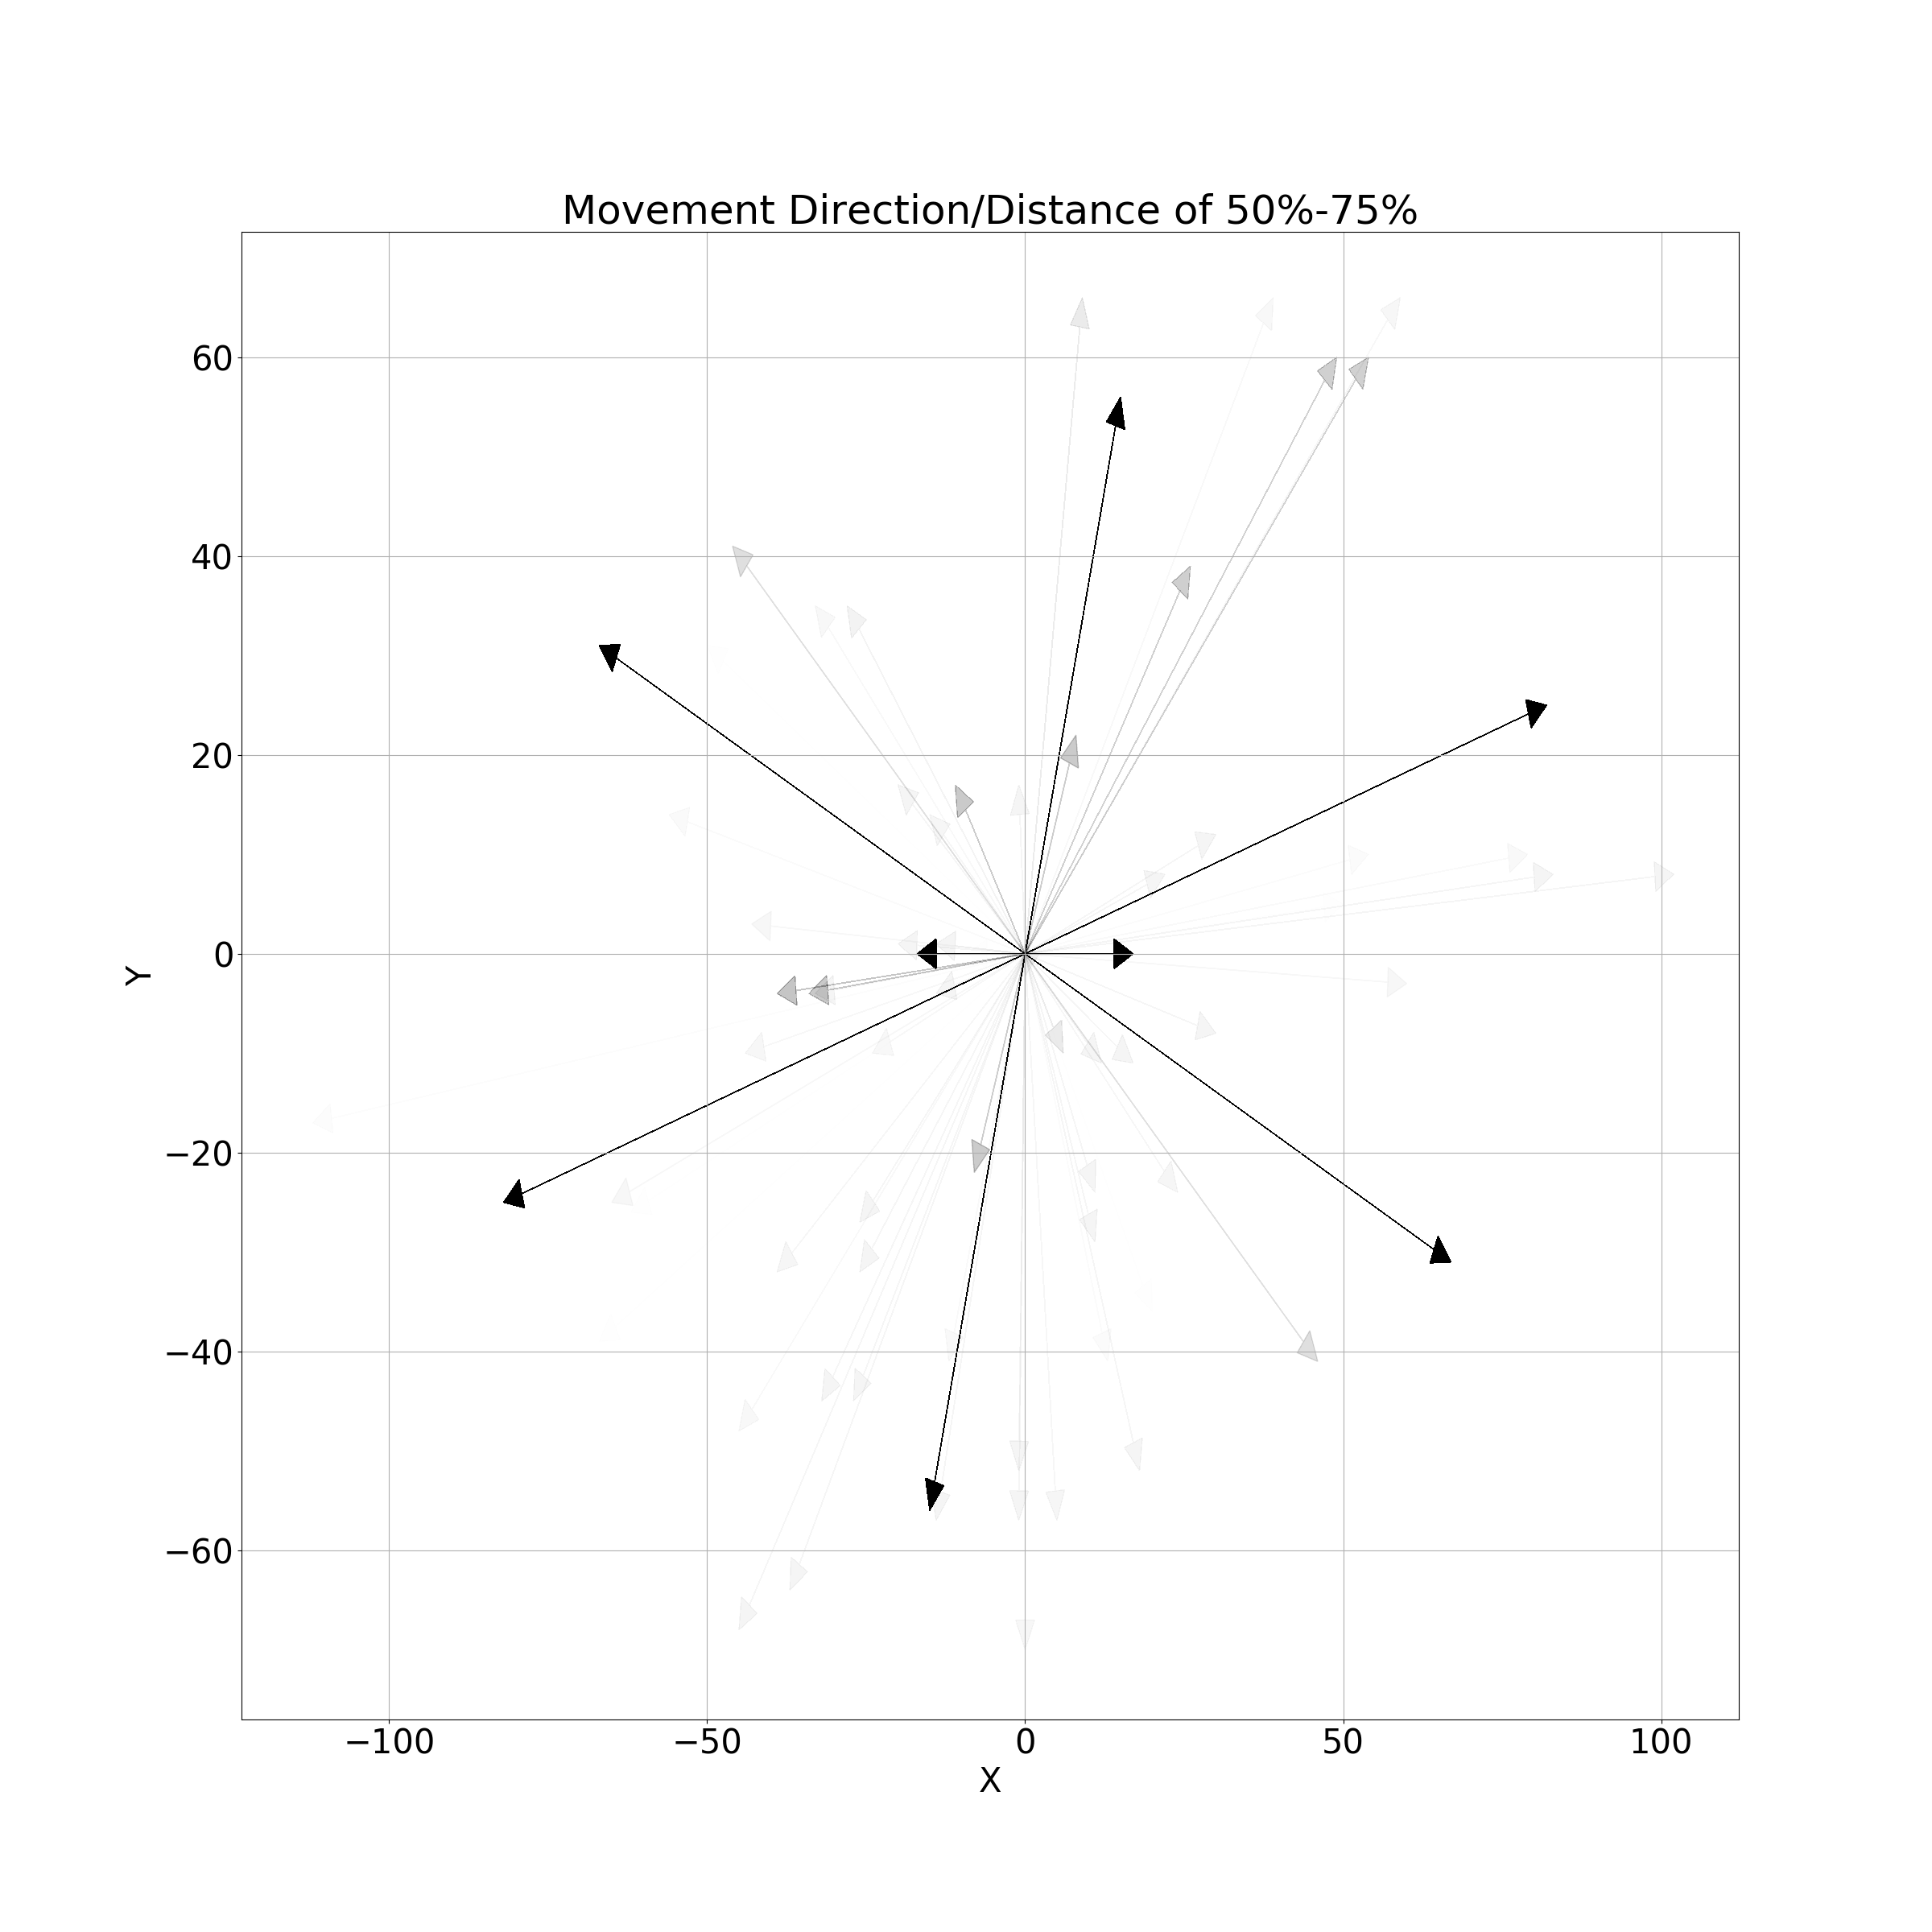
\includegraphics[width=0.3 \linewidth]{figures/movement2-3.png}
                    &
                    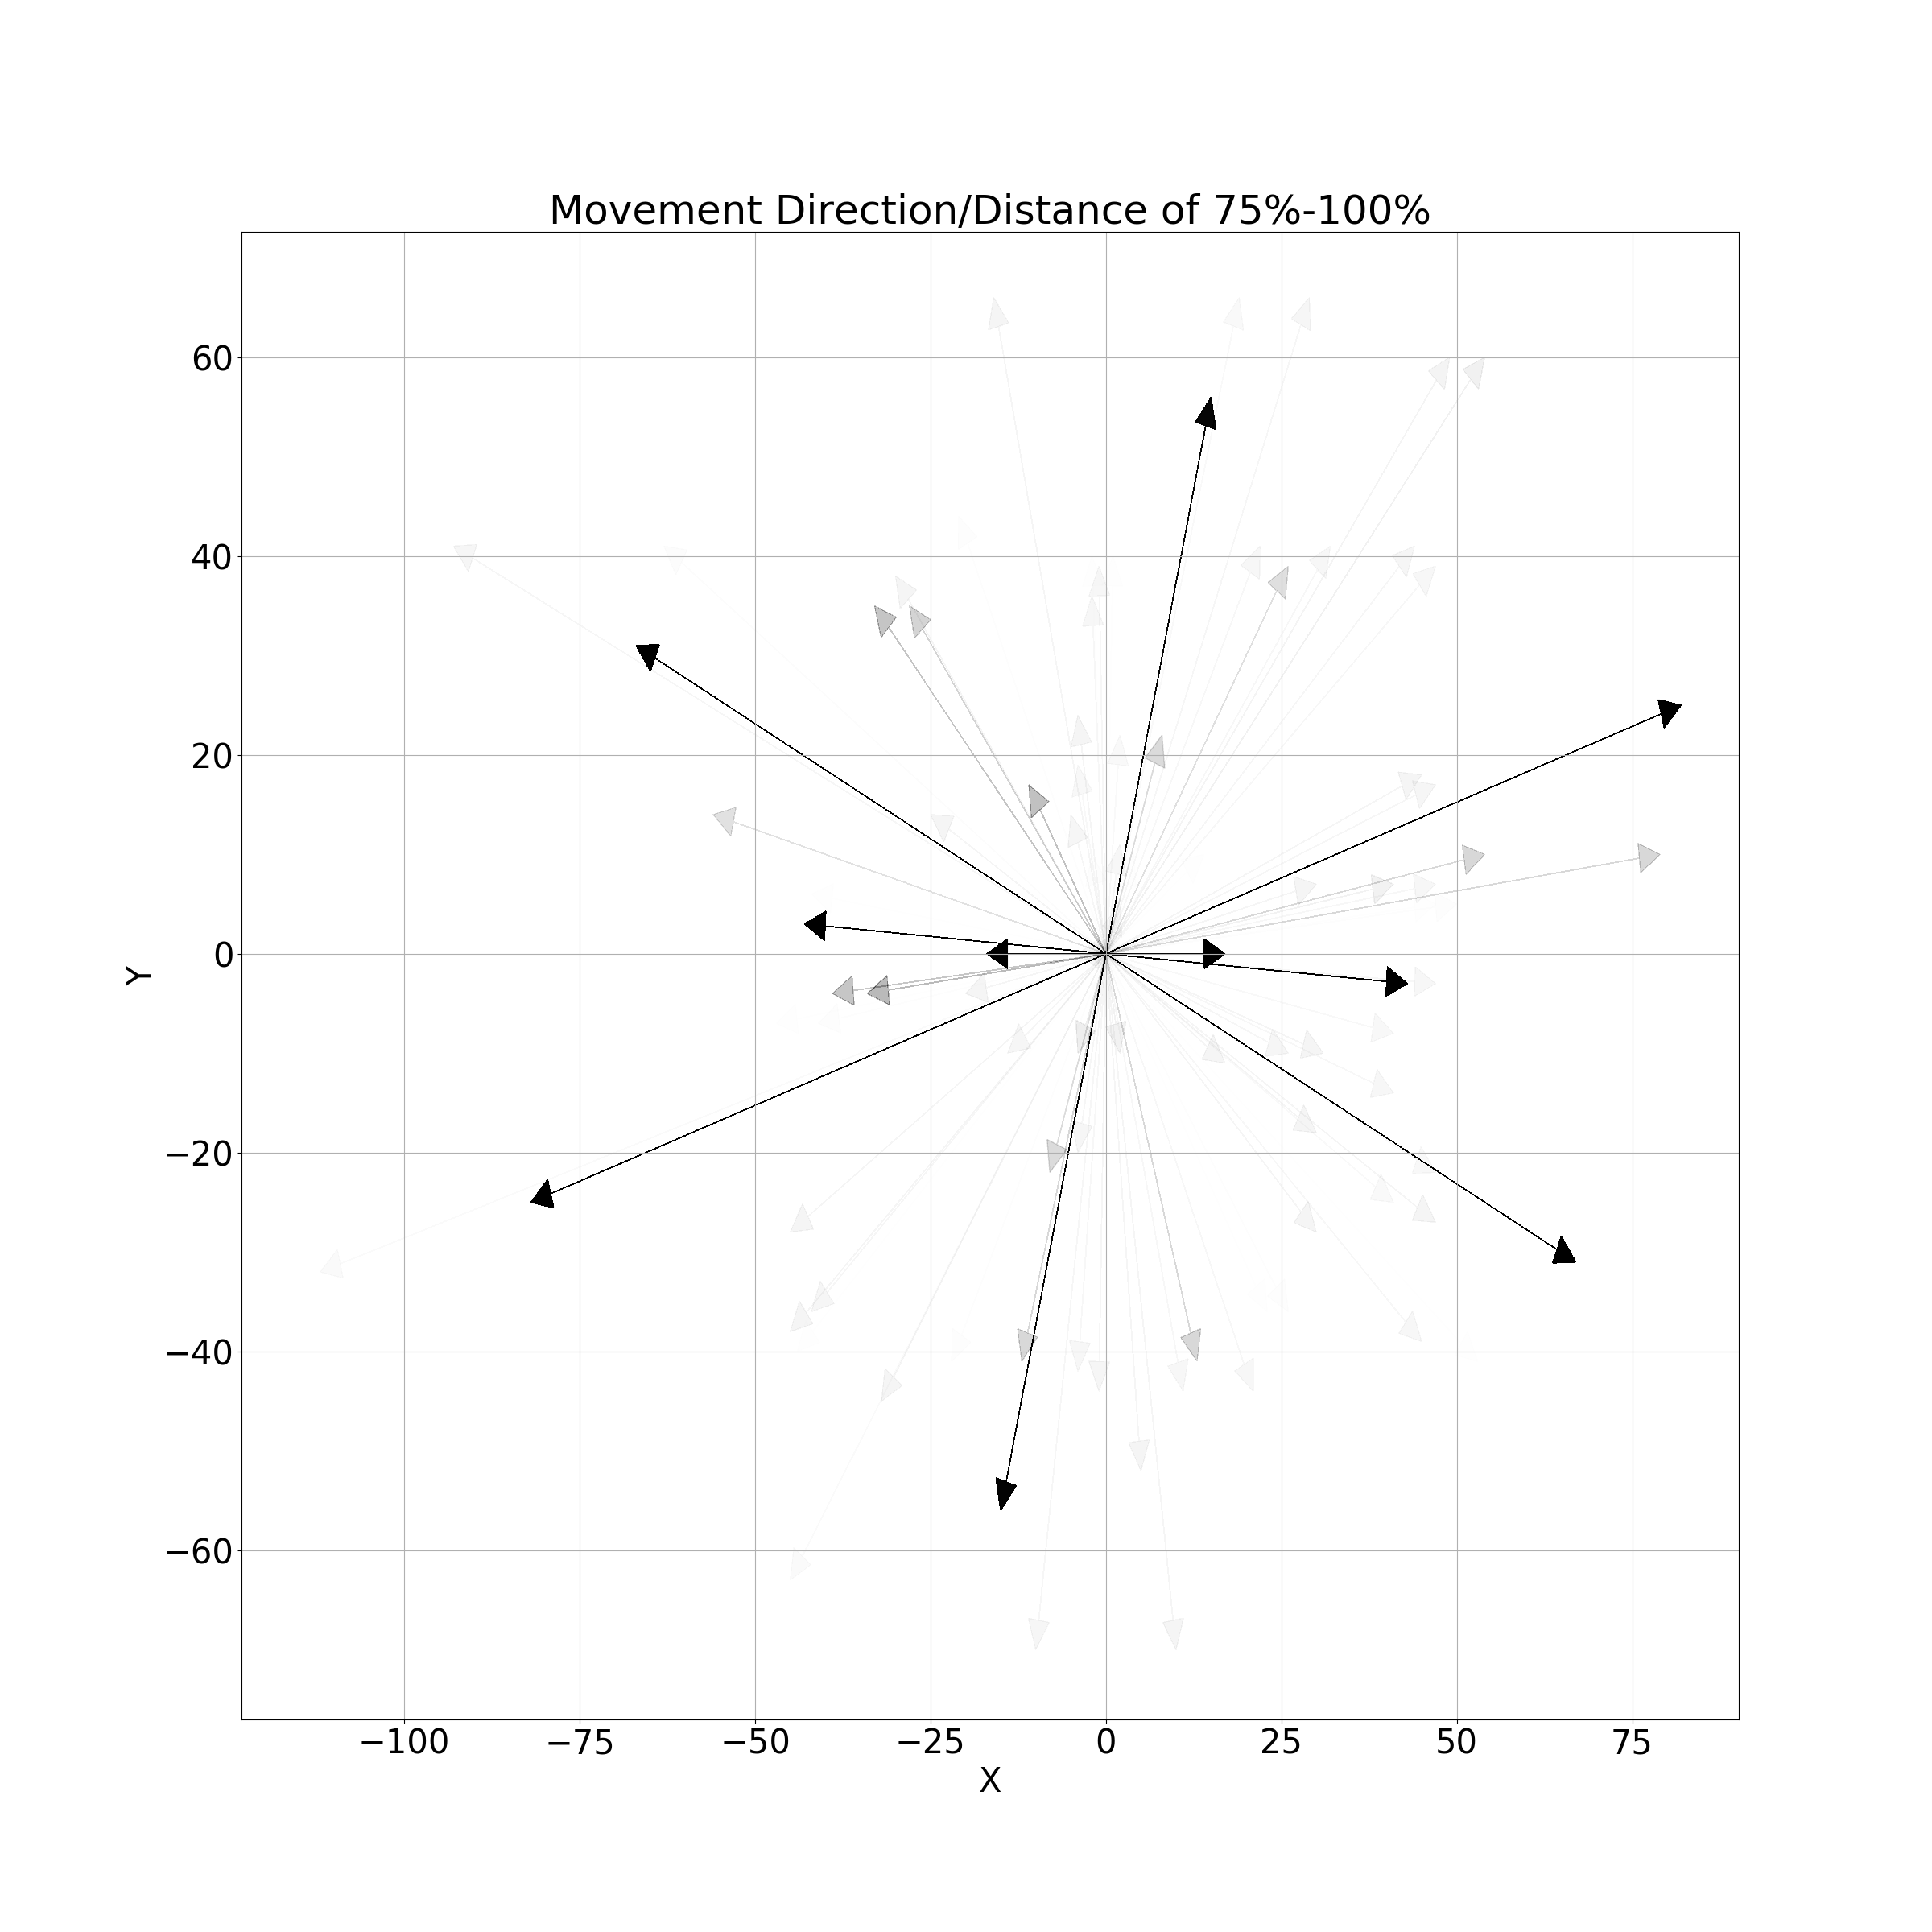
\includegraphics[width=0.3 \linewidth]{figures/movement2-4.png}
                    \\
                    
                    \mbox{(c) 50\%-75\%} & \mbox{(d) 75\%-100\%} \\
                \end{array}$
                \caption{Movement Direction/Distance on Second Floor}
                \label{fig:movedd2}
                \end{figure}
            
                \begin{figure}[htbp]
                    \centering
                    $\begin{array}{cc}
                    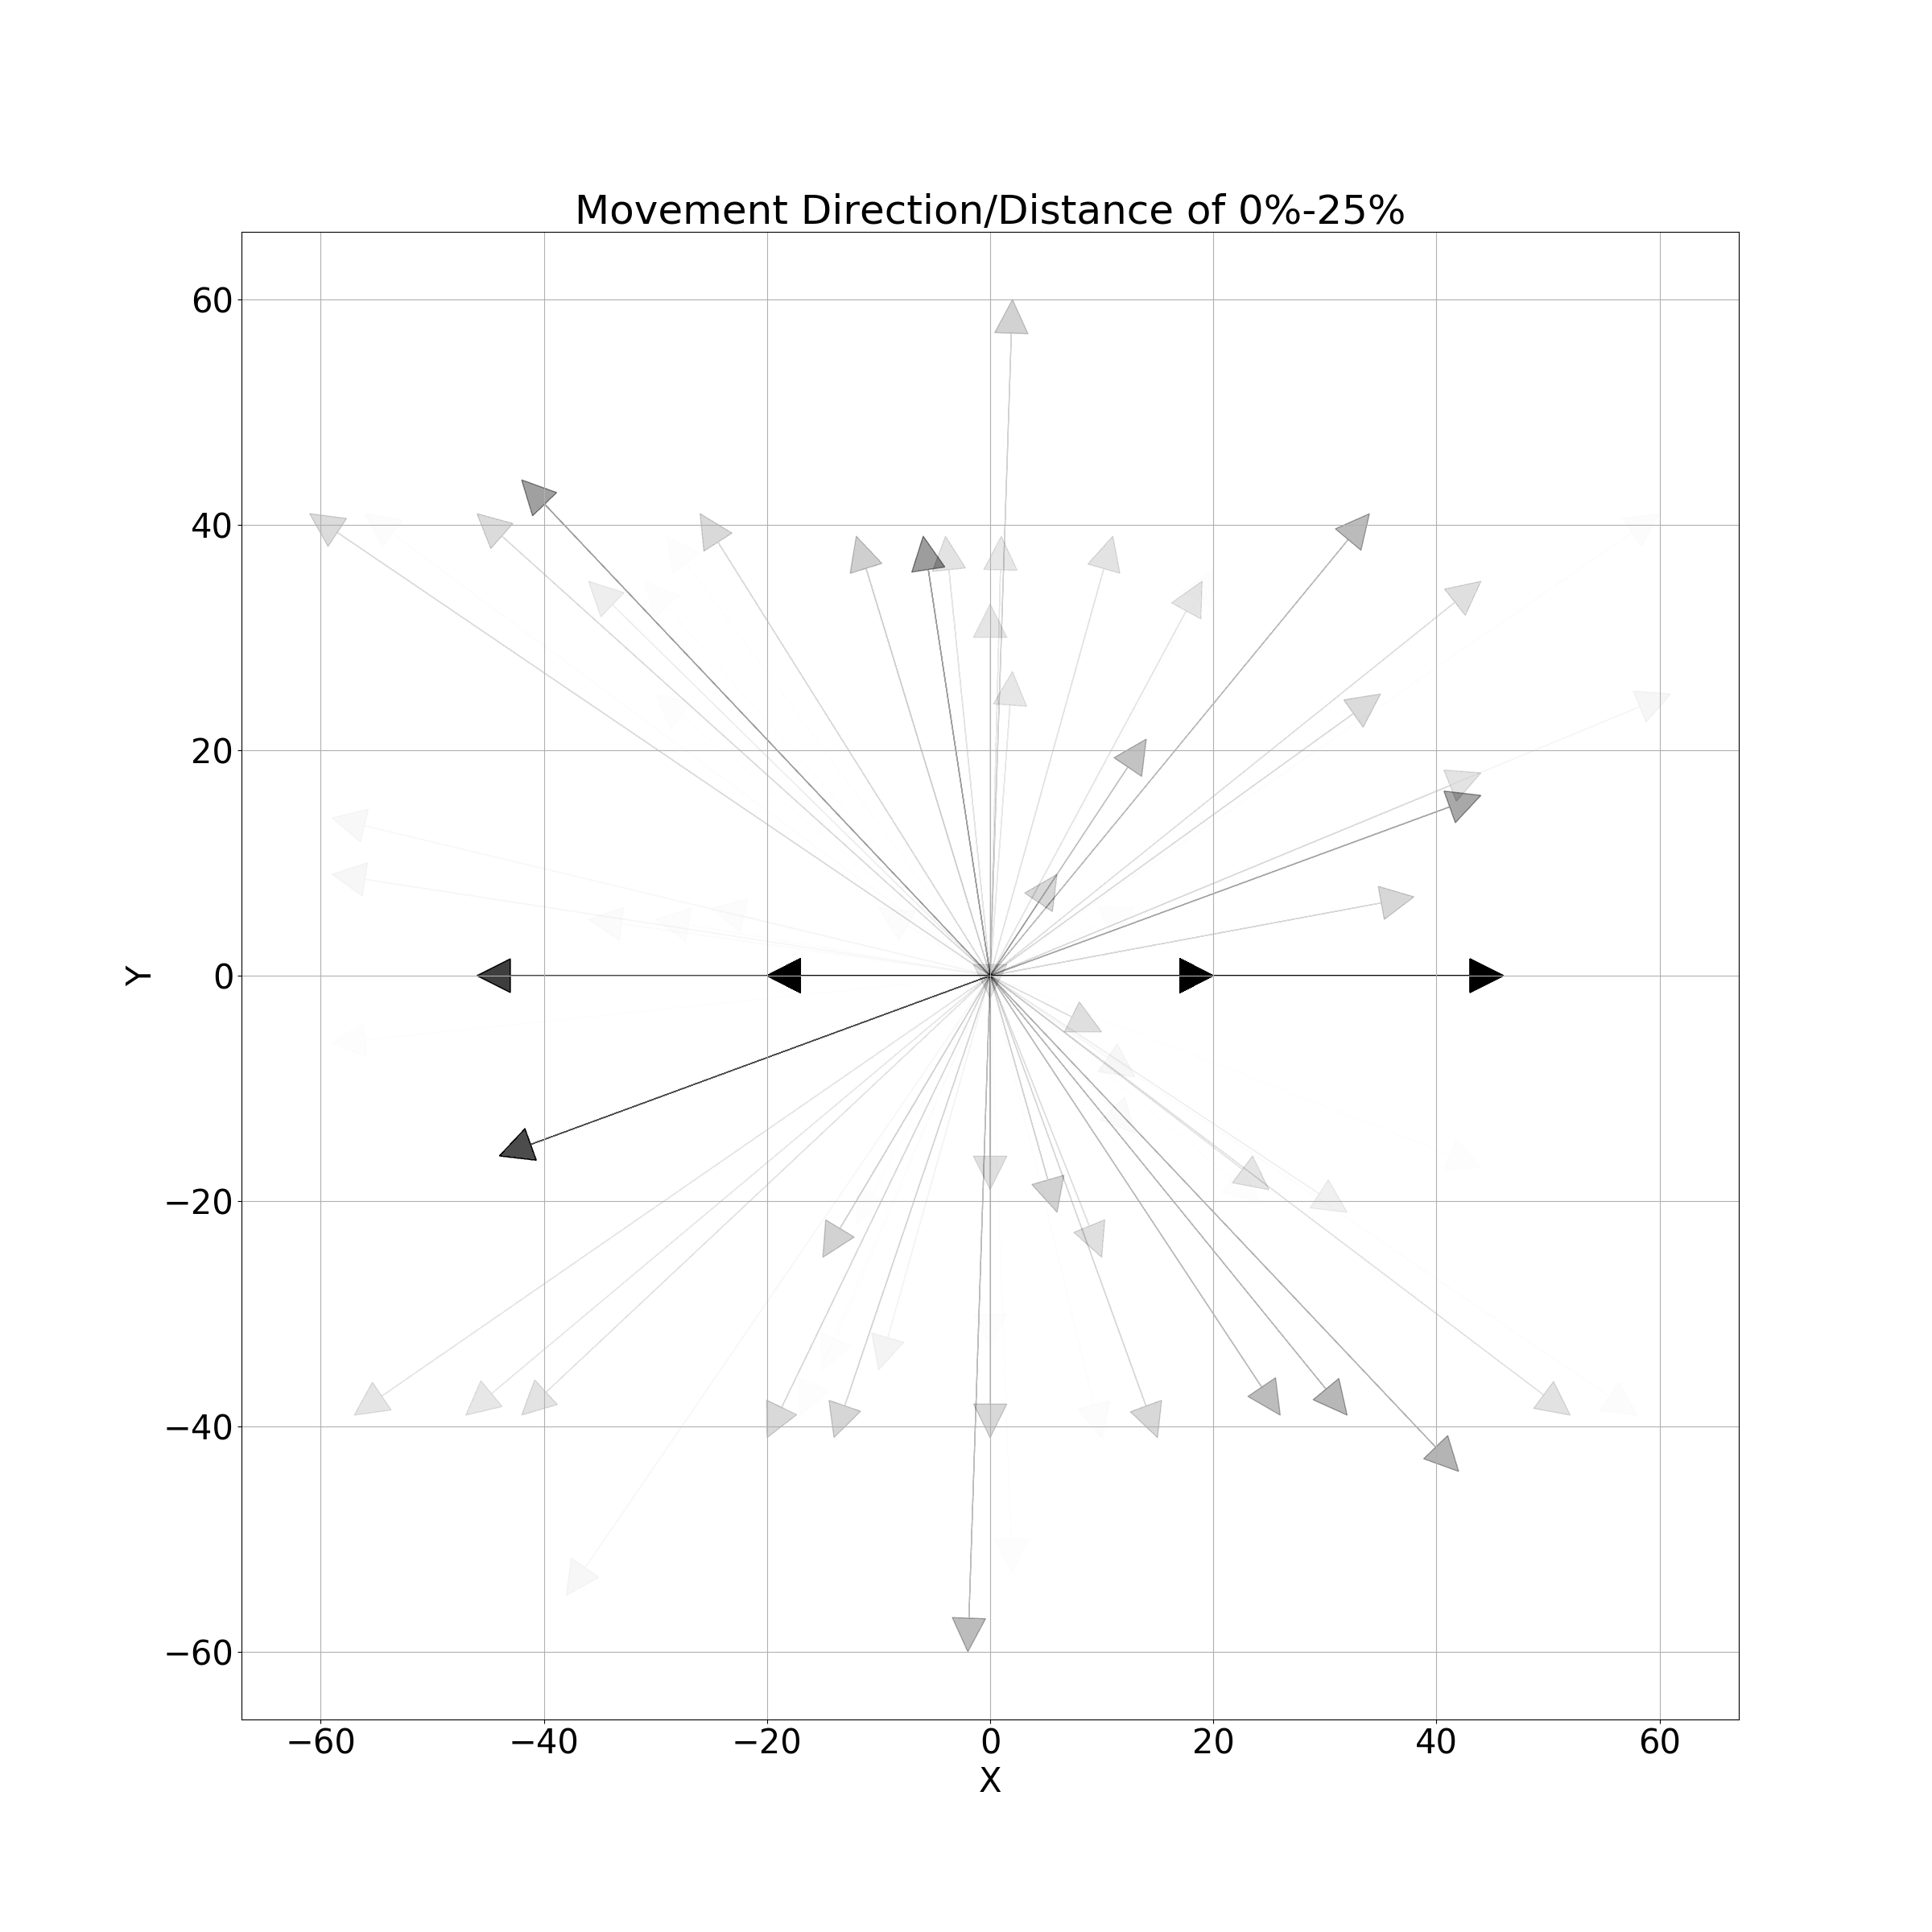
\includegraphics[width=0.3 \linewidth]{figures/movement3-1.png}
                    &
                    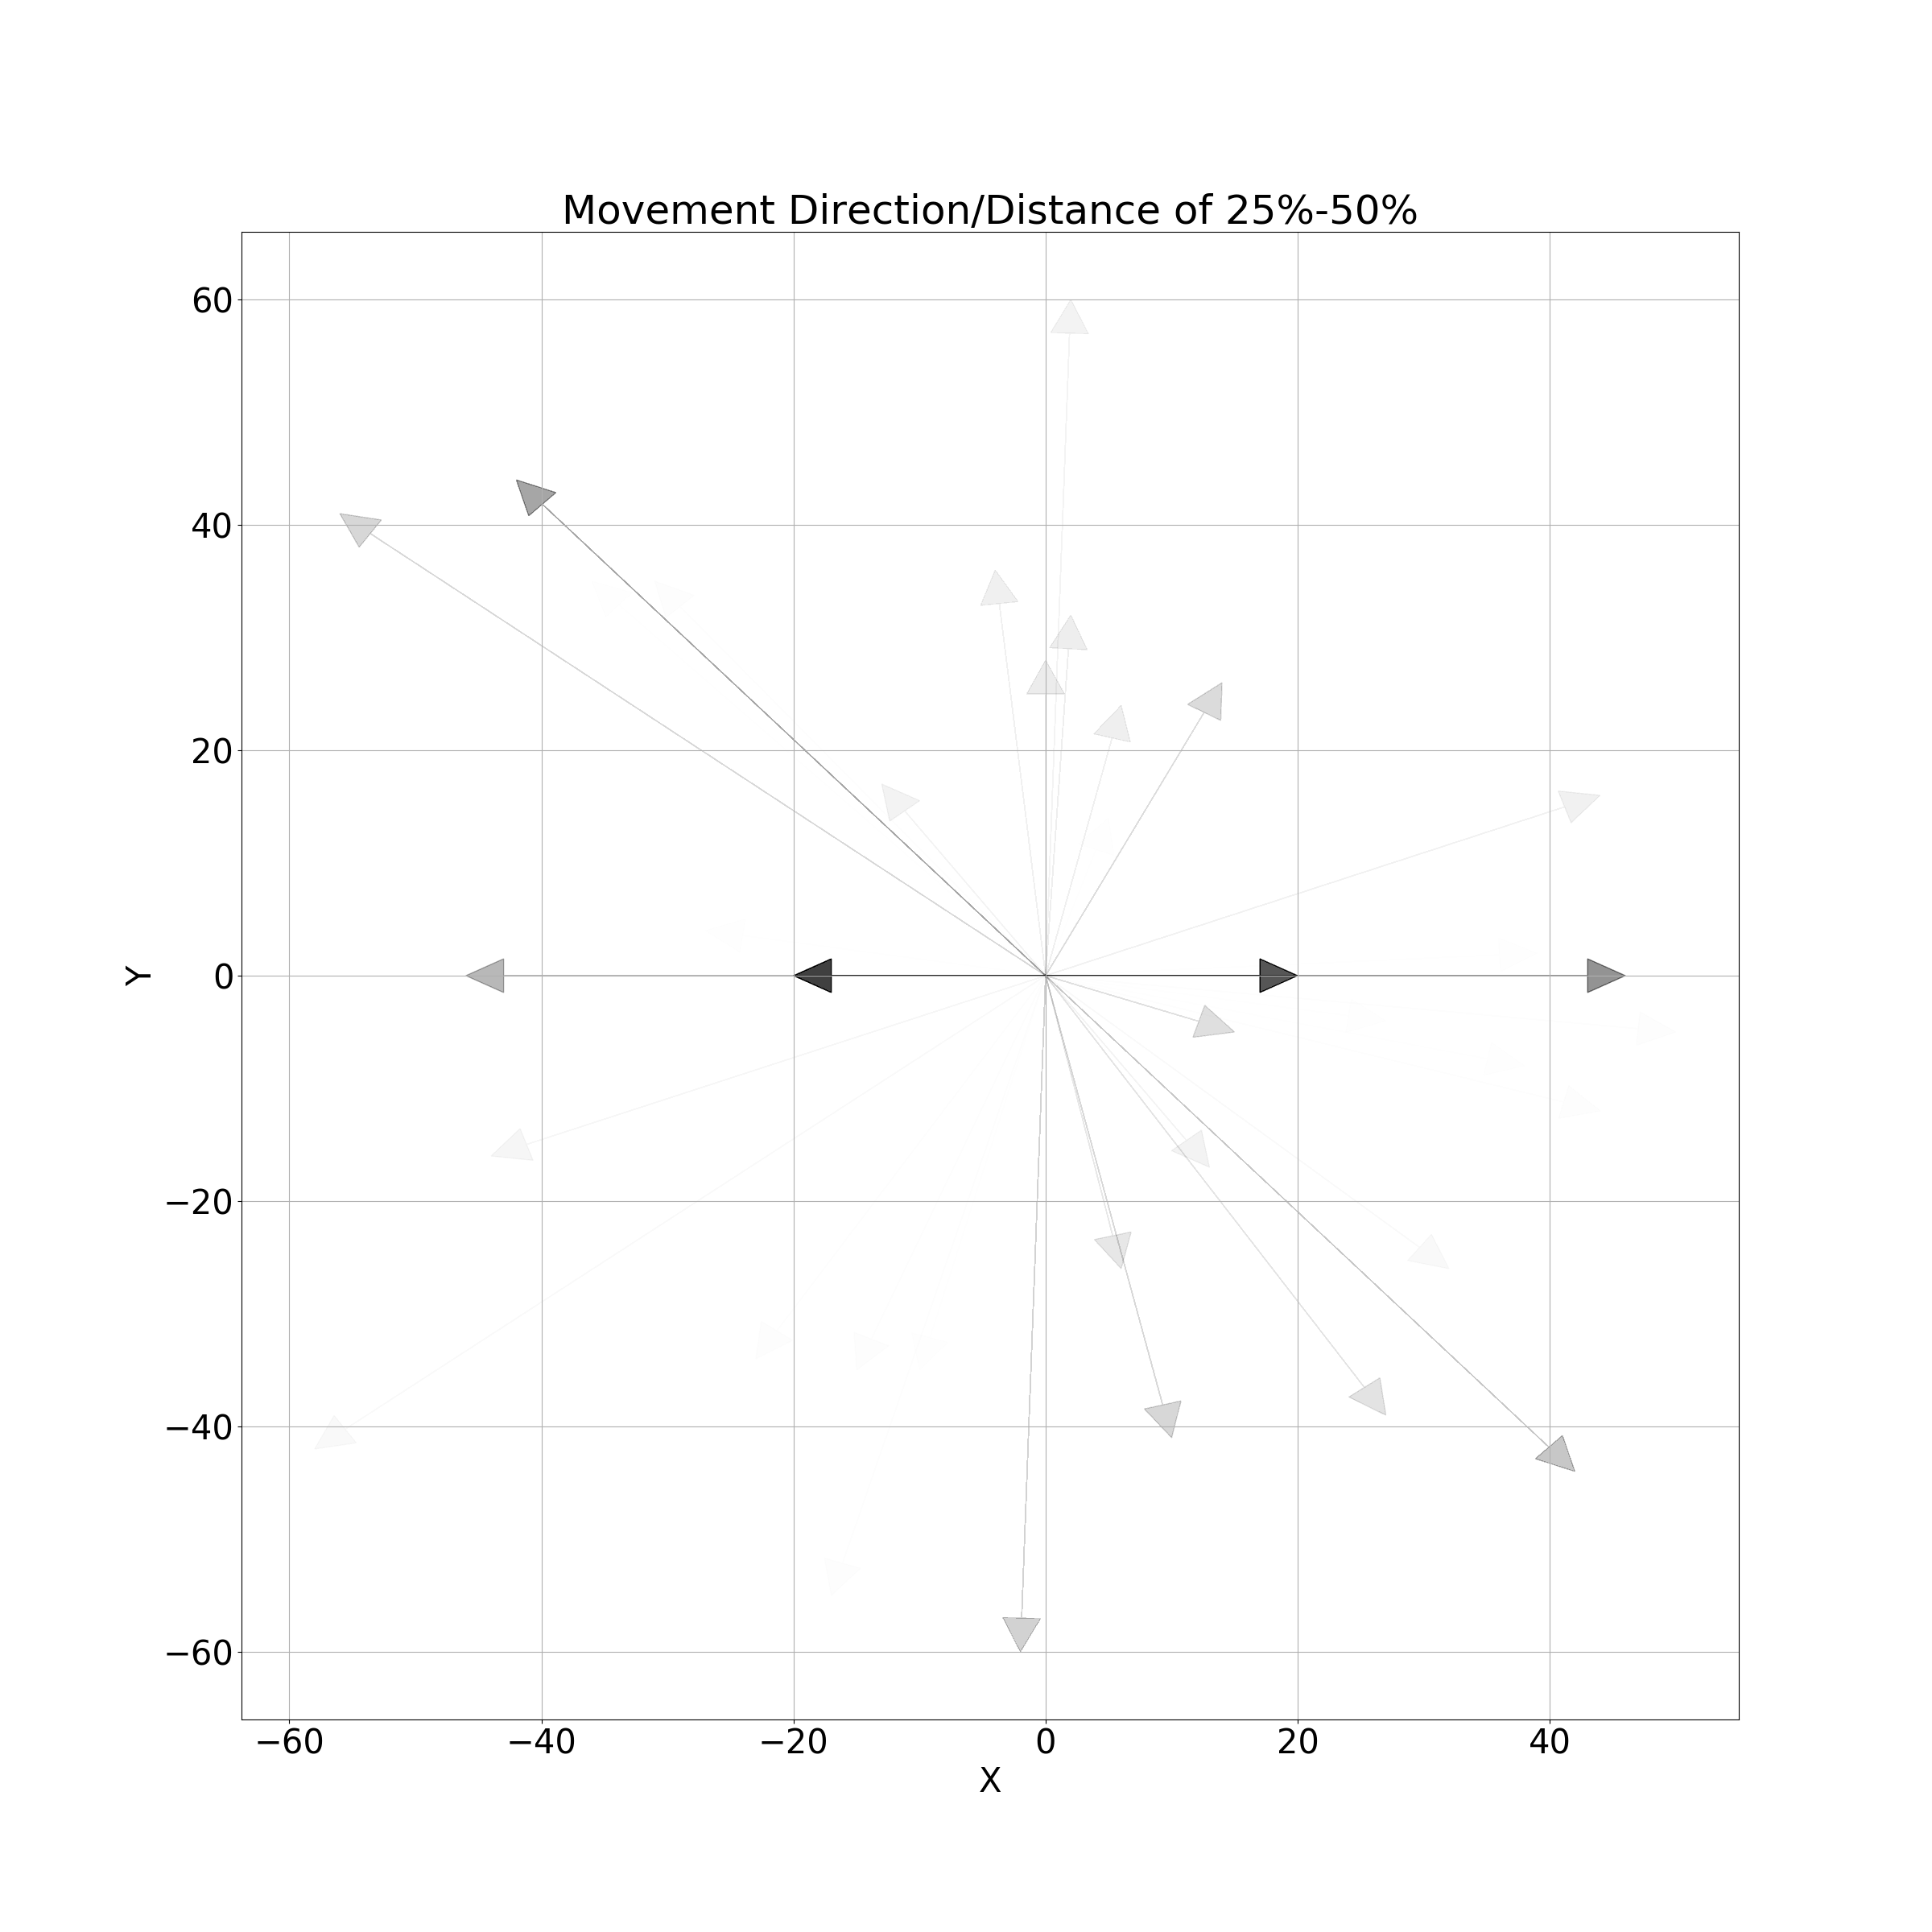
\includegraphics[width=0.3 \linewidth]{figures/movement3-2.png}
                    \\
                    
                    \mbox{(a) 0\%-25\%} & \mbox{(b) 25\%-50\%} \\
                    
                    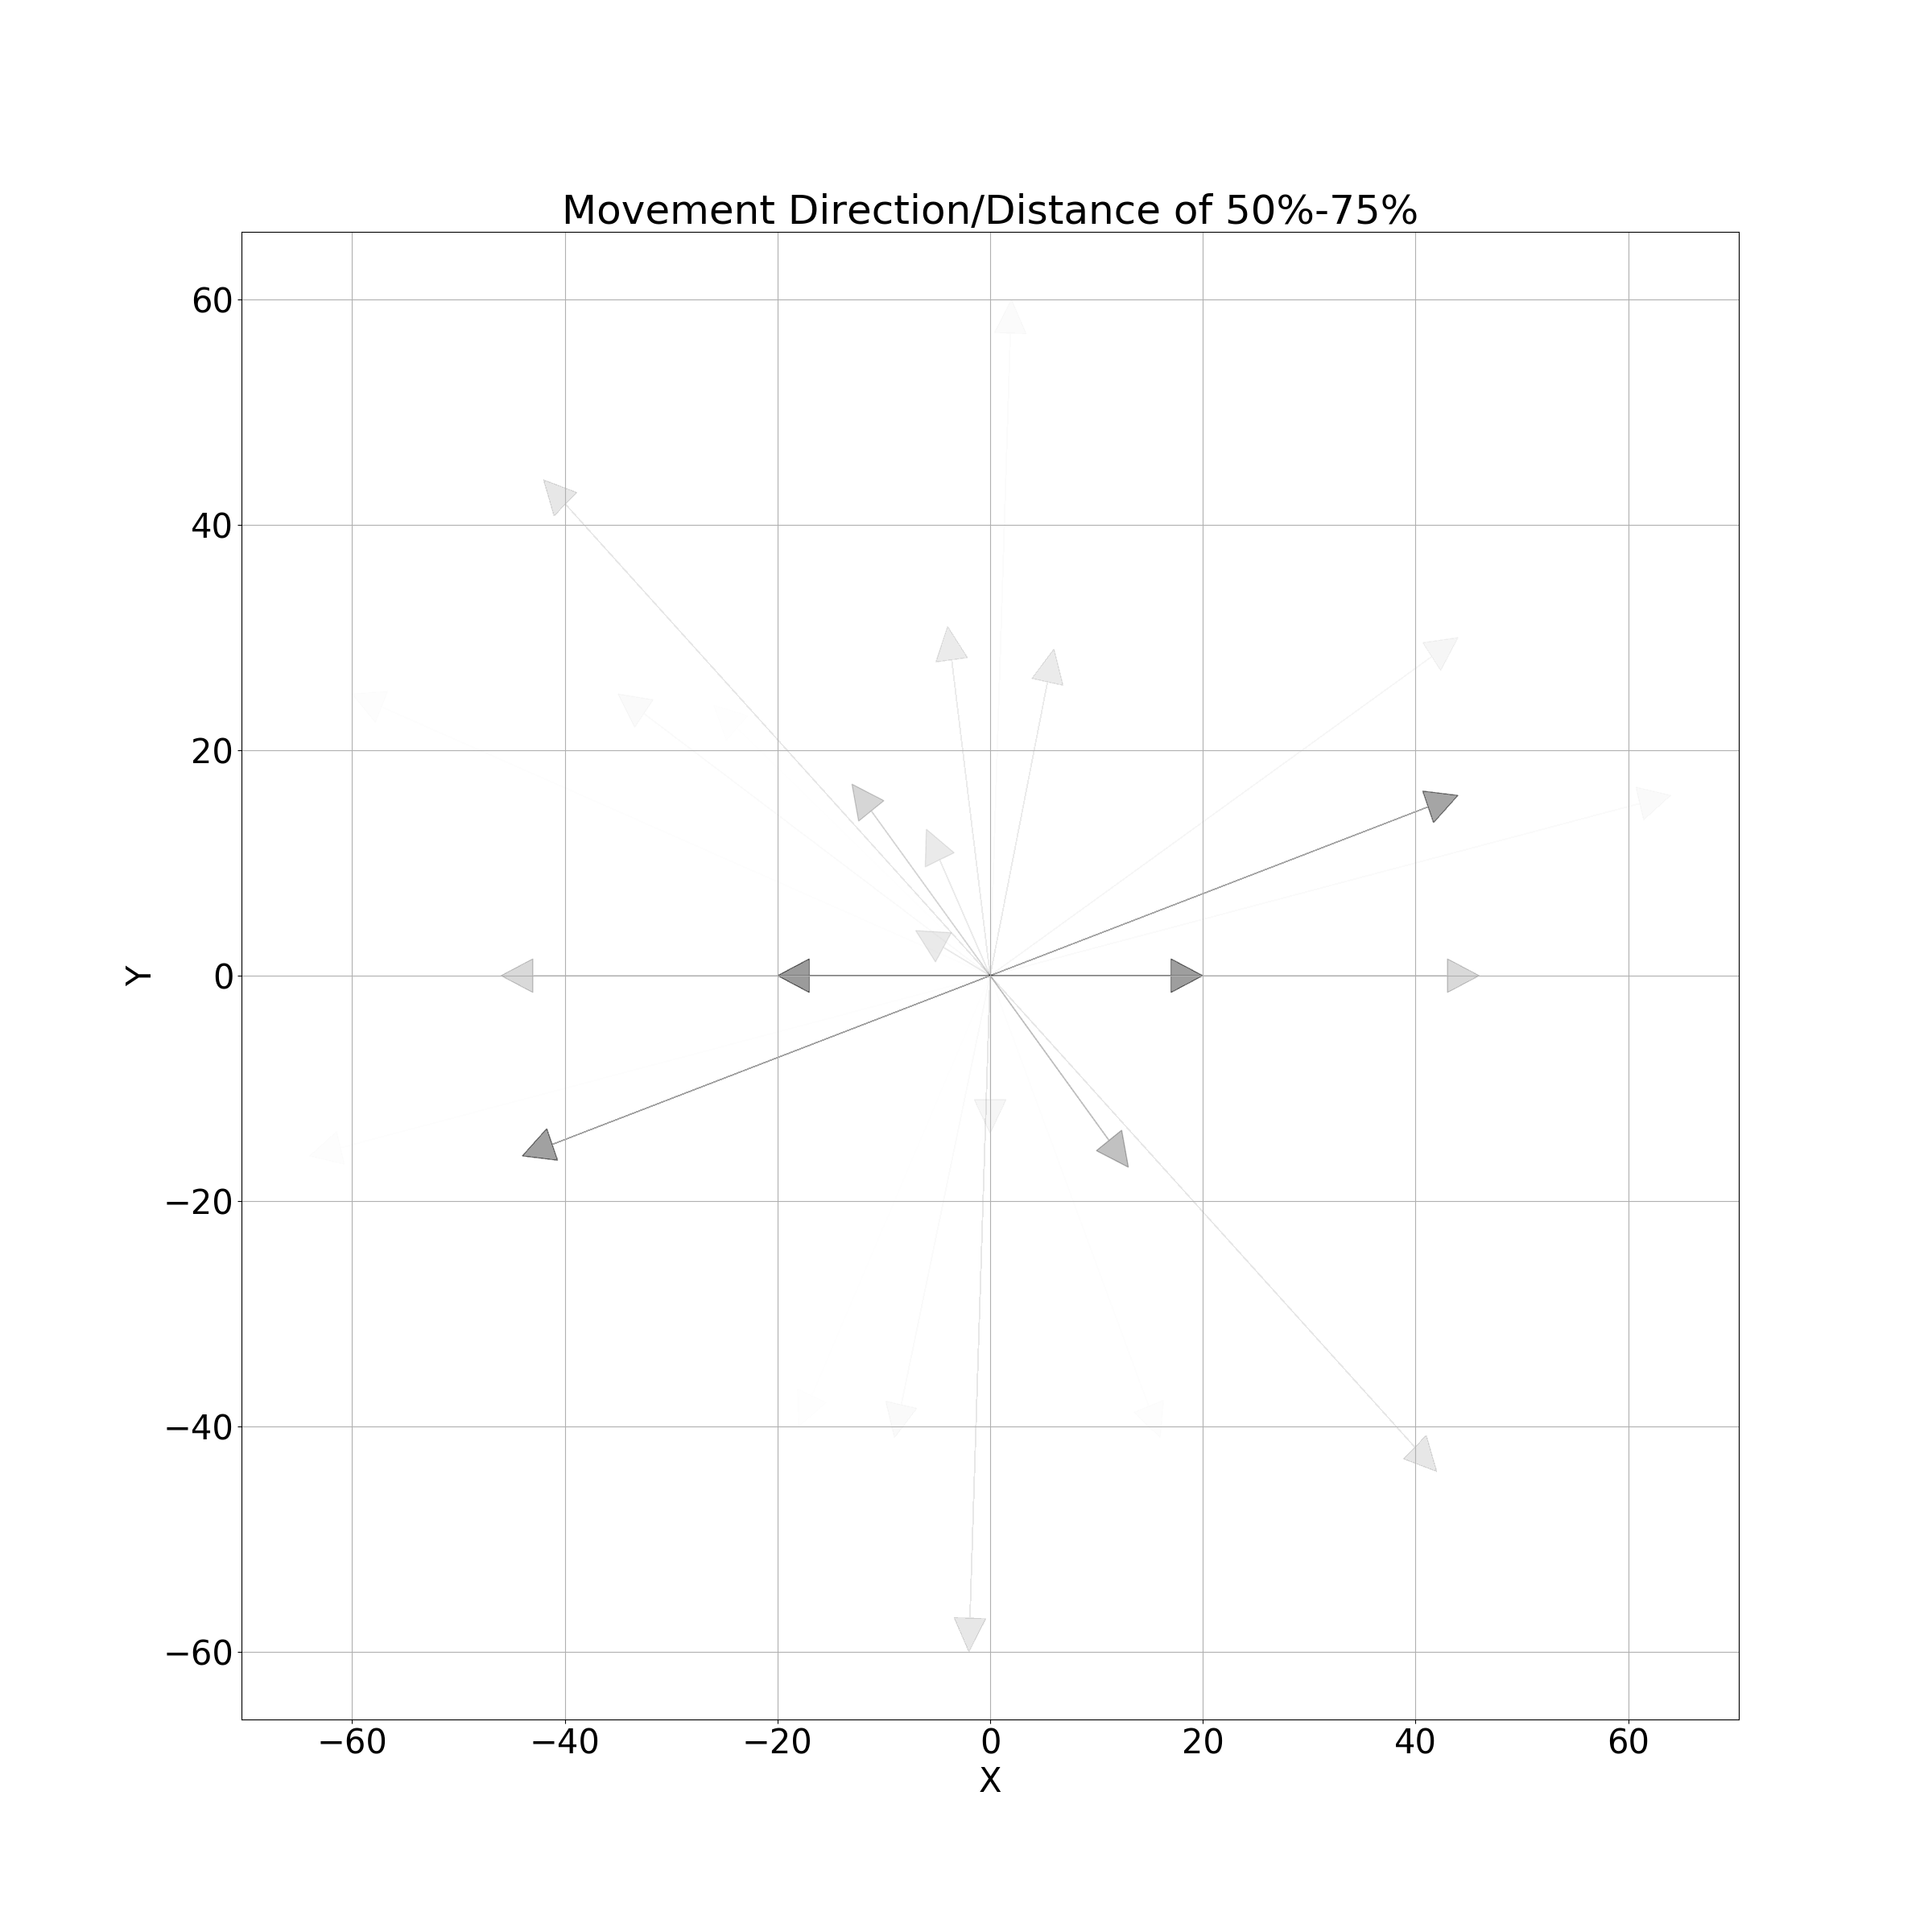
\includegraphics[width=0.3 \linewidth]{figures/movement3-3.png}
                    &
                    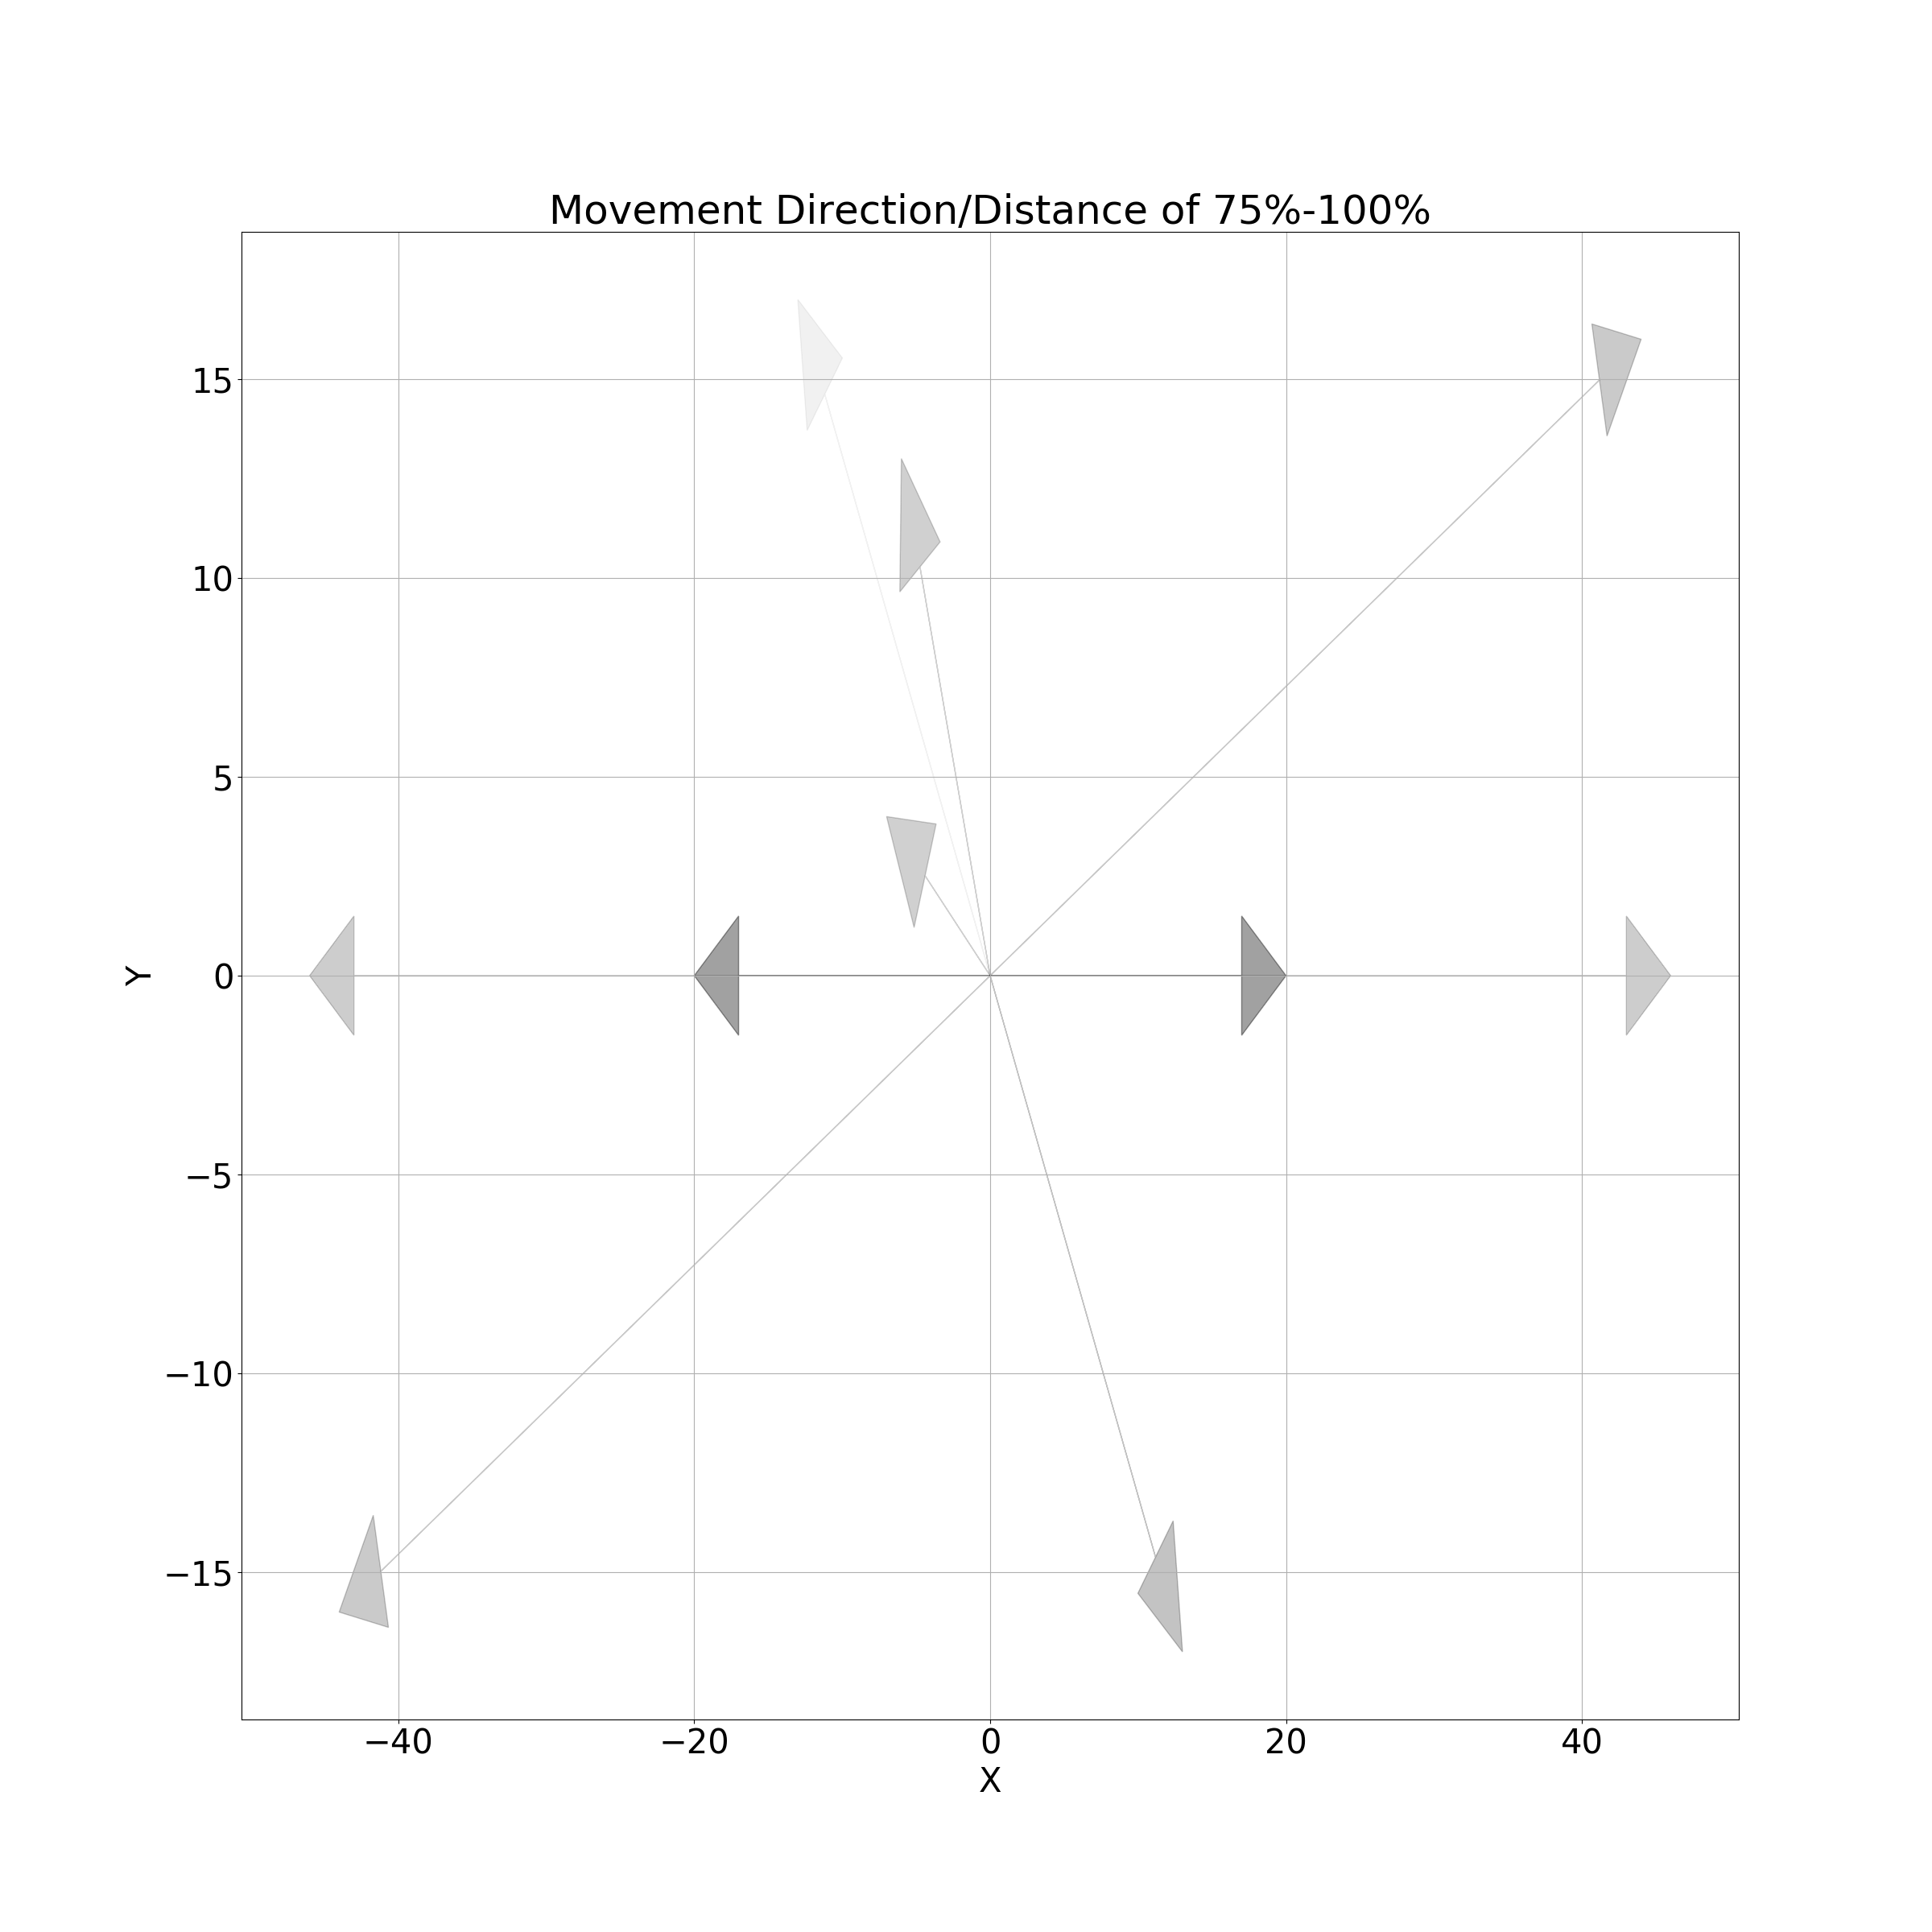
\includegraphics[width=0.3 \linewidth]{figures/movement3-4.png}
                    \\
                    
                    \mbox{(c) 50\%-75\%} & \mbox{(d) 75\%-100\%} \\
                \end{array}$
                \caption{Movement Direction/Distance on Third Floor}
                \label{fig:movedd3}
                \end{figure}
            
        
        \subsection[Question 2]{Describe up to five of the most interesting patterns that appear in the building data. Describe what is notable about the pattern and explain its possible significance.}
            \subsubsection{General Information of Building Data}
                First of all, we drew the distribution of the building data using TSNE technique. The TSNE plot of general building data is shows as figure \ref{fig:generalbuilding}.
            
                \begin{figure}[htbp]
                    \centering
                    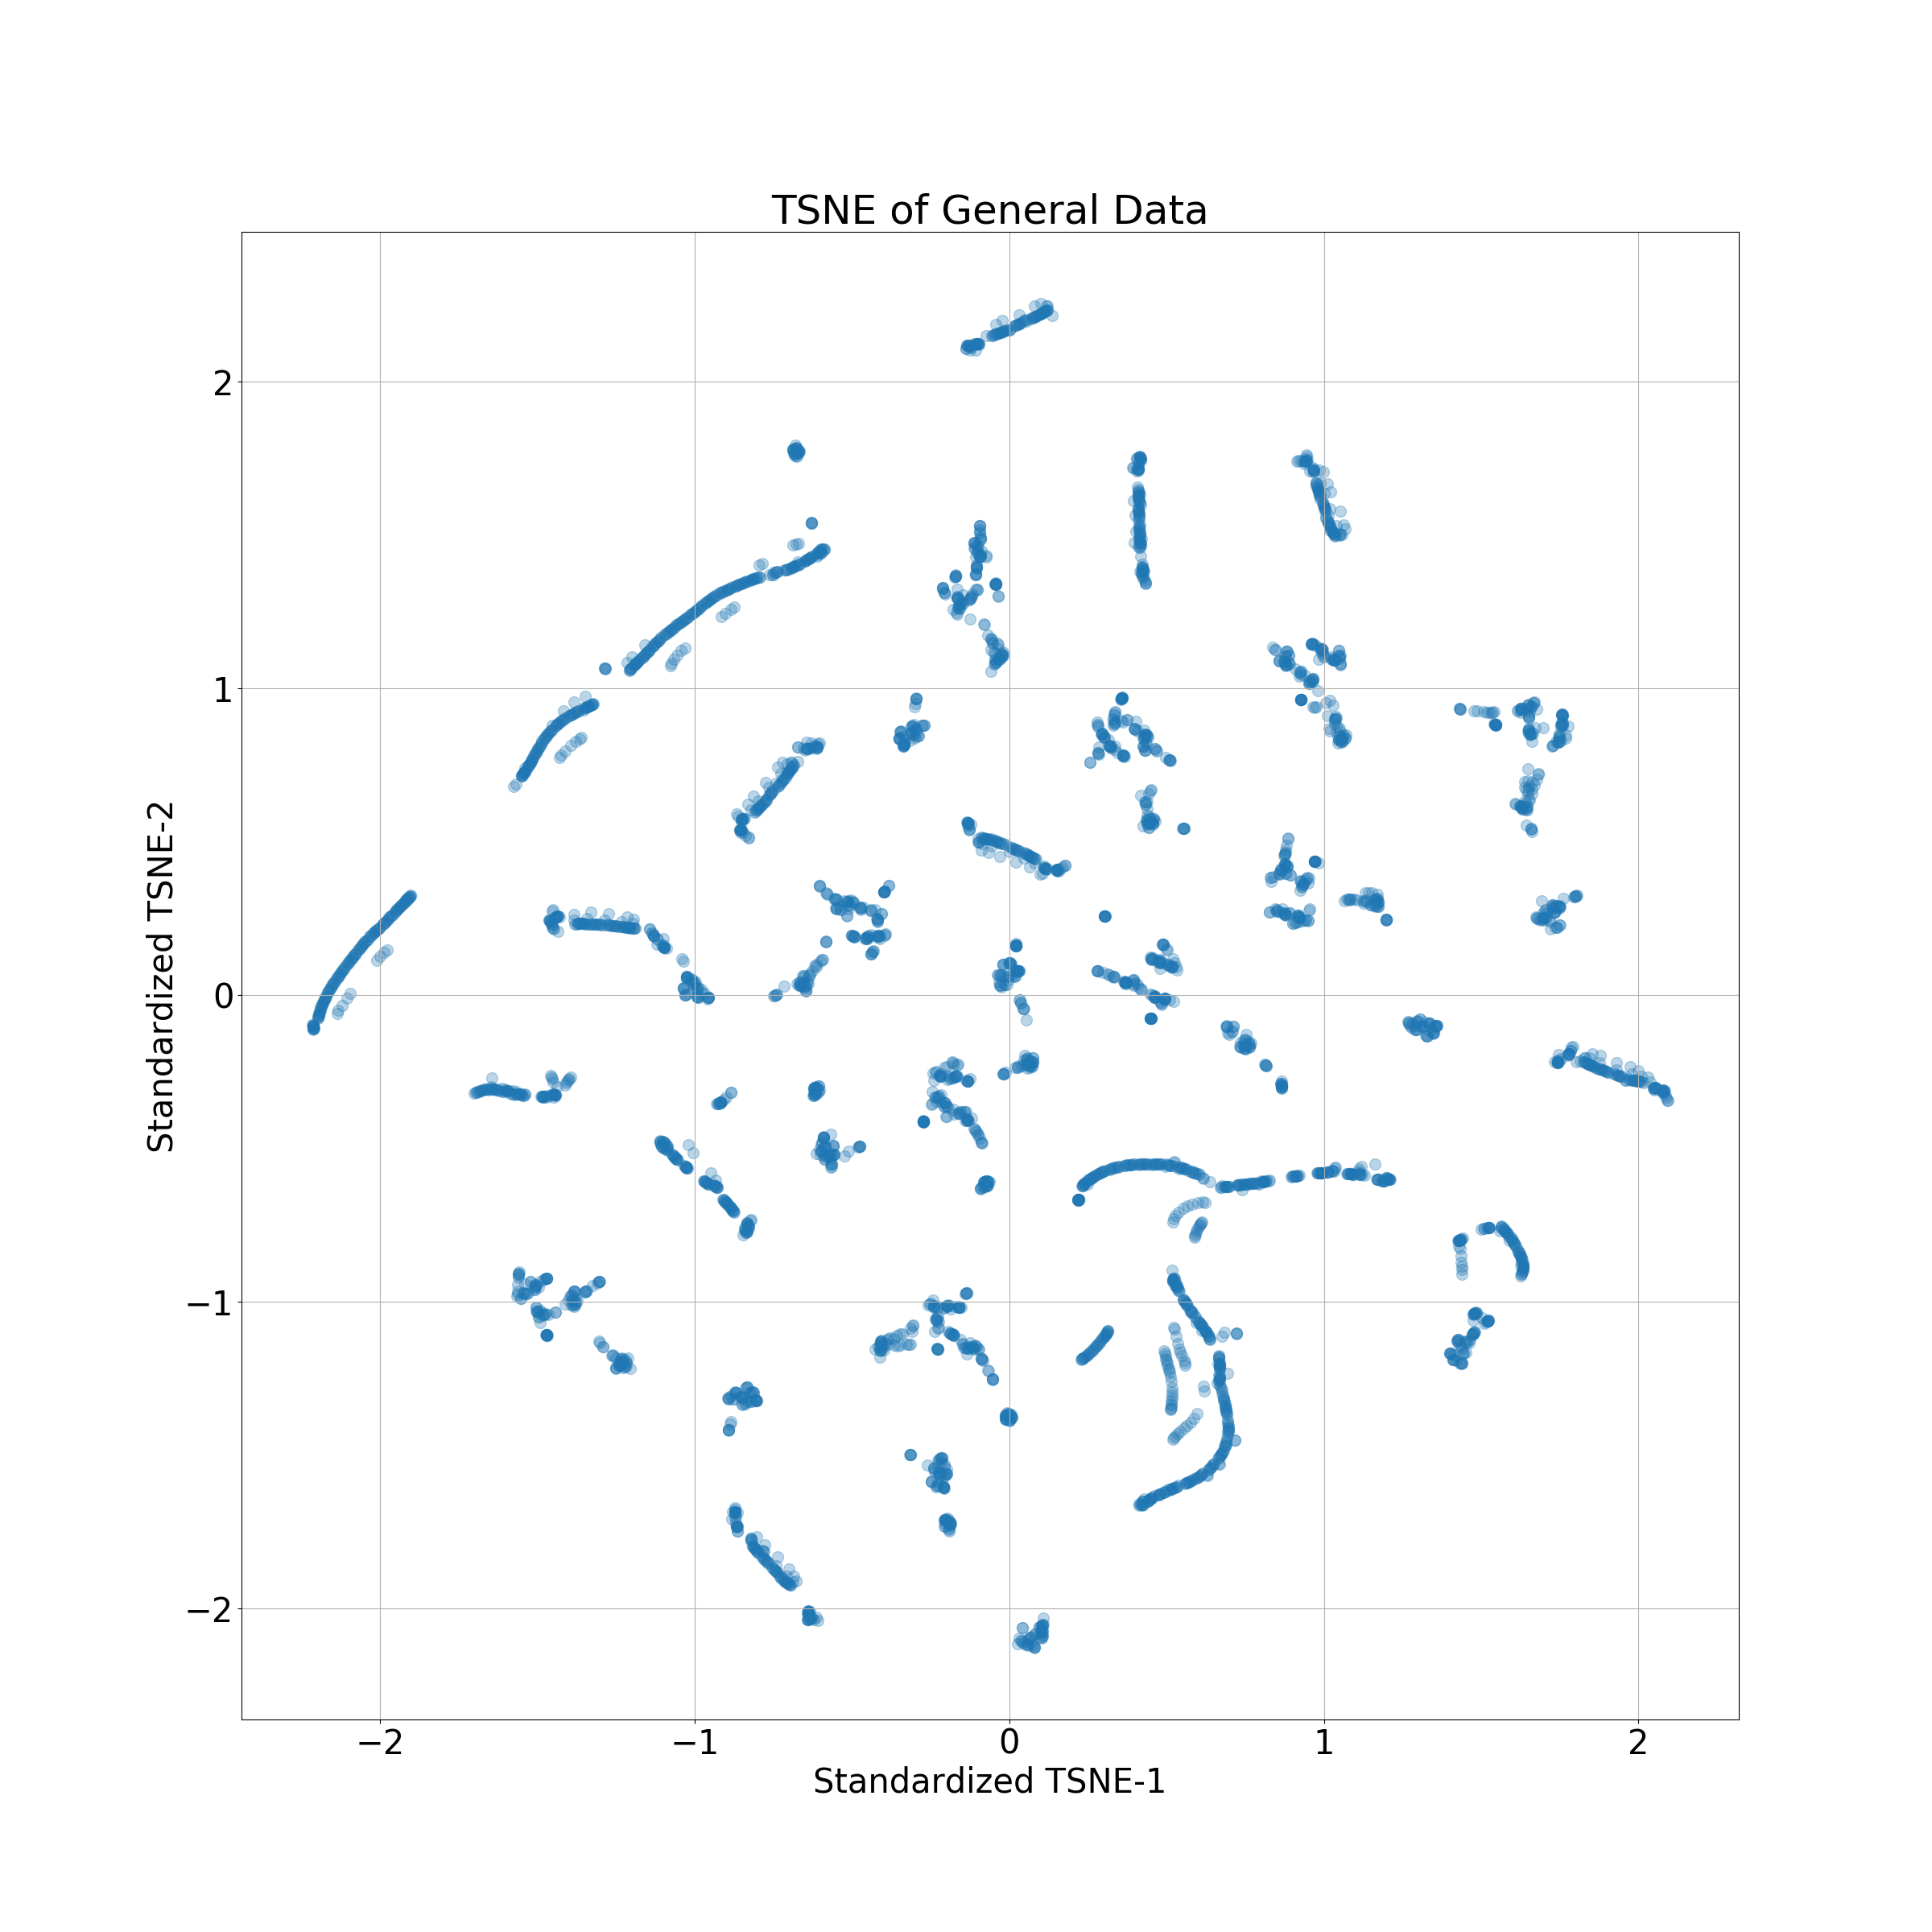
\includegraphics[width=0.3 \linewidth]{figures/TsneGeneral.png}
                    \caption{TSNE Plot for General Building Data}
                    \label{fig:generalbuilding}
                \end{figure}
            
            \subsubsection{Workflow}
 
            \subsubsection{Find Abnormality}       
                To find patterns which appear in the building data, we should find that normality/abnormality in the building data. However, there are over 400 columns in the general building data; therefore, it is almost impossible to find abnormality column-by-column by human. Hence, we used these four algorithms which are included in scikit-learn: \textit{EllipticEnvelope} \cite{ref:normal1}, \textit{OneClassSVM}, \textit{IsolationForest} \cite{ref:normal2, ref:normal3}, and \textit{LocalOutlierFactor} \cite{ref:normal4}.
            
                \begin{figure}[htbp]
                    \centering
                    $\begin{array}{cc}
                        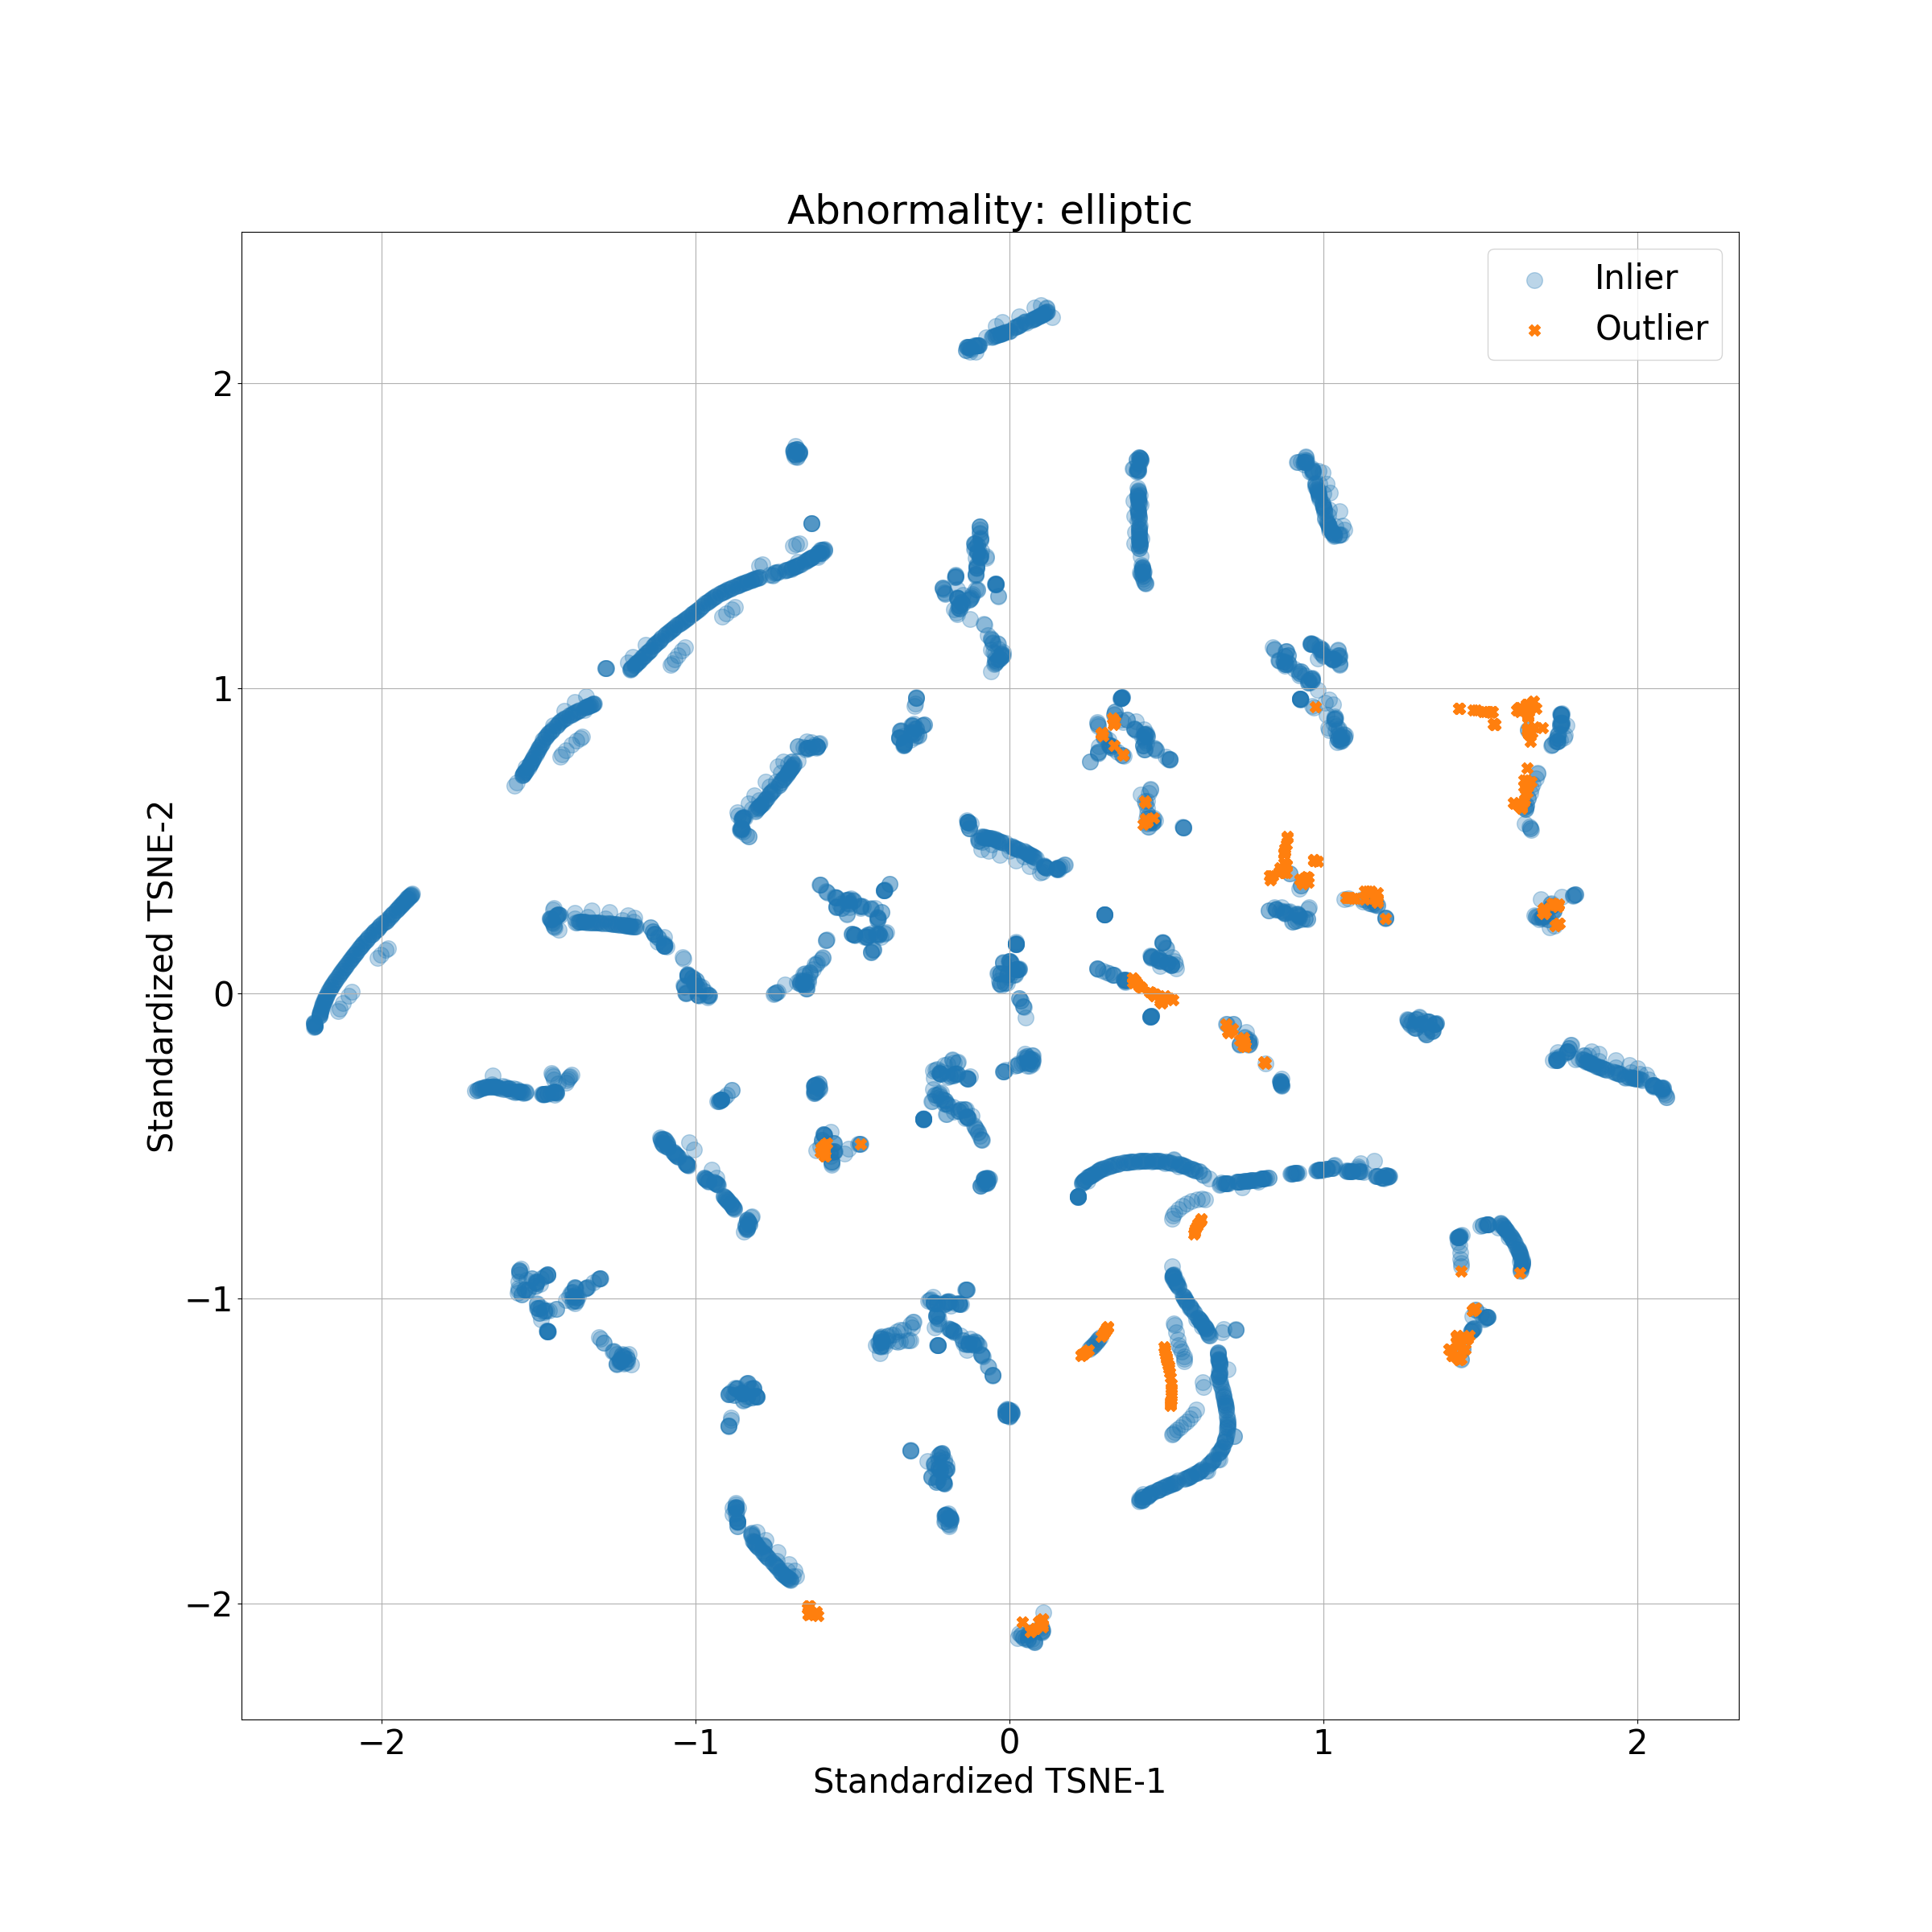
\includegraphics[width=0.3 \linewidth]{figures/outlier1.png}
                        &
                        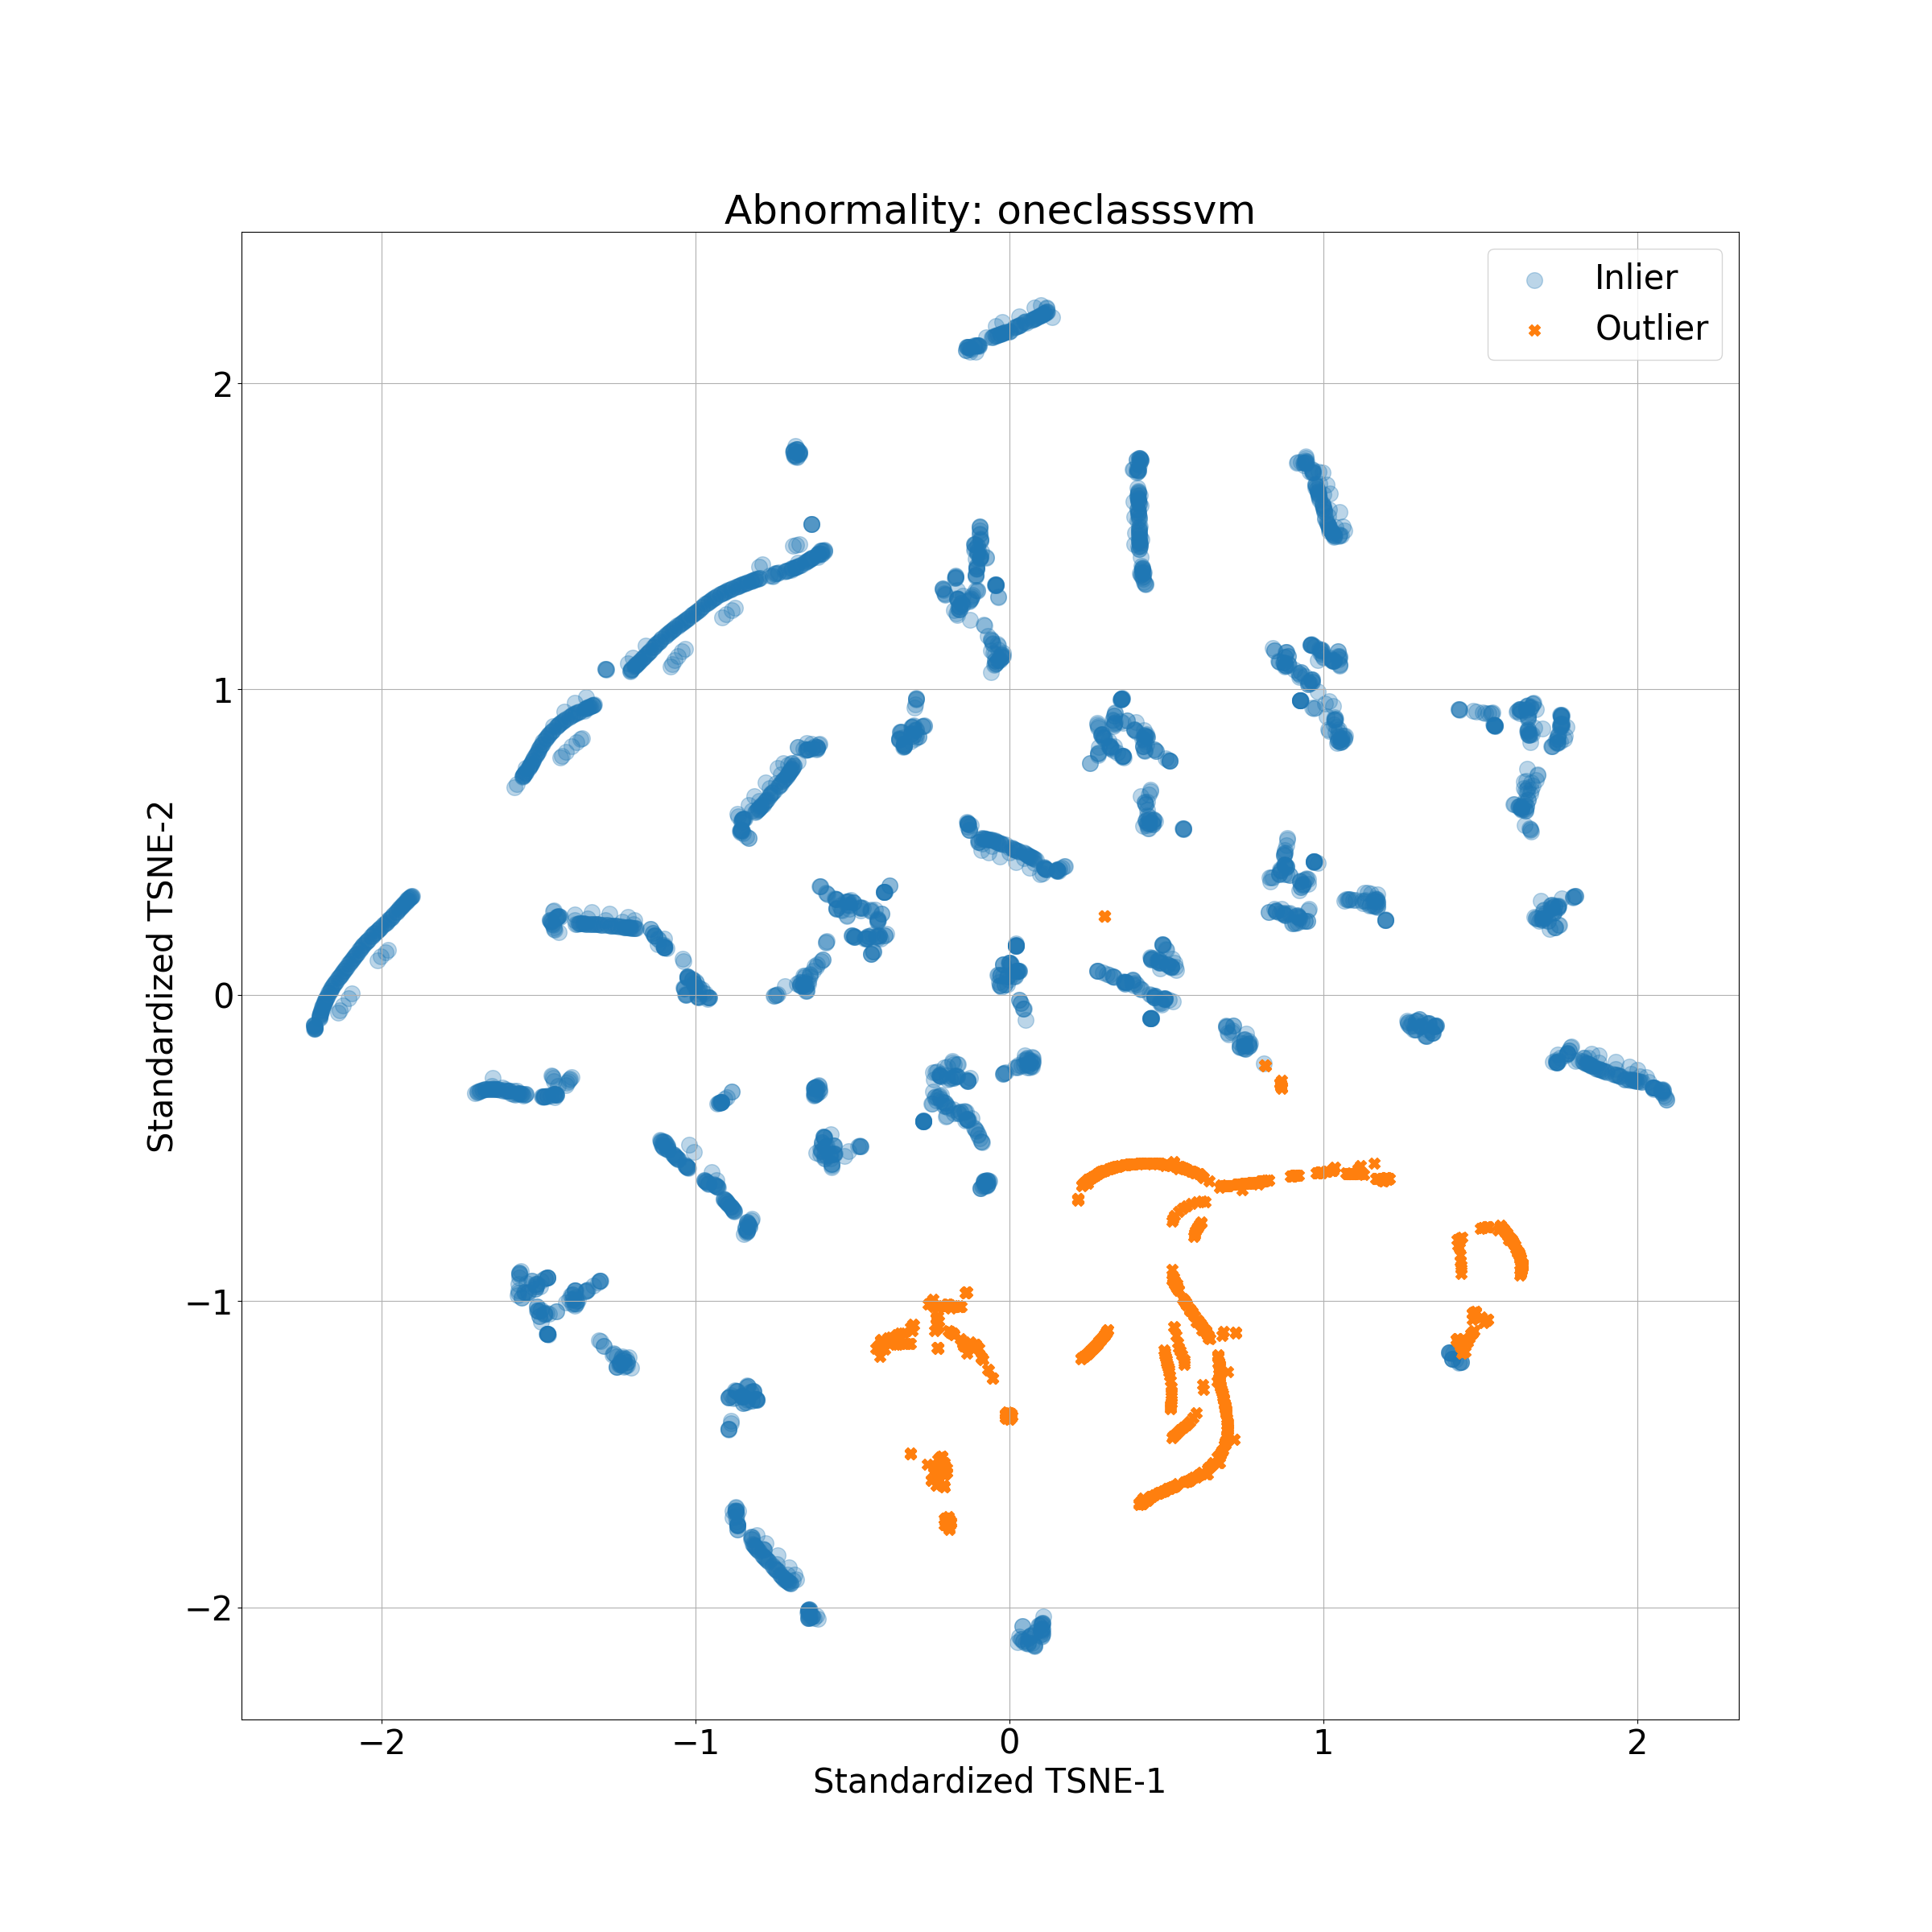
\includegraphics[width=0.3 \linewidth]{figures/outlier2.png}
                        \\
                        
                        \mbox{(a) \textit{EllipticEnvelope}} & \mbox{(b) \textit{OneClassSVM}} \\
                        
                        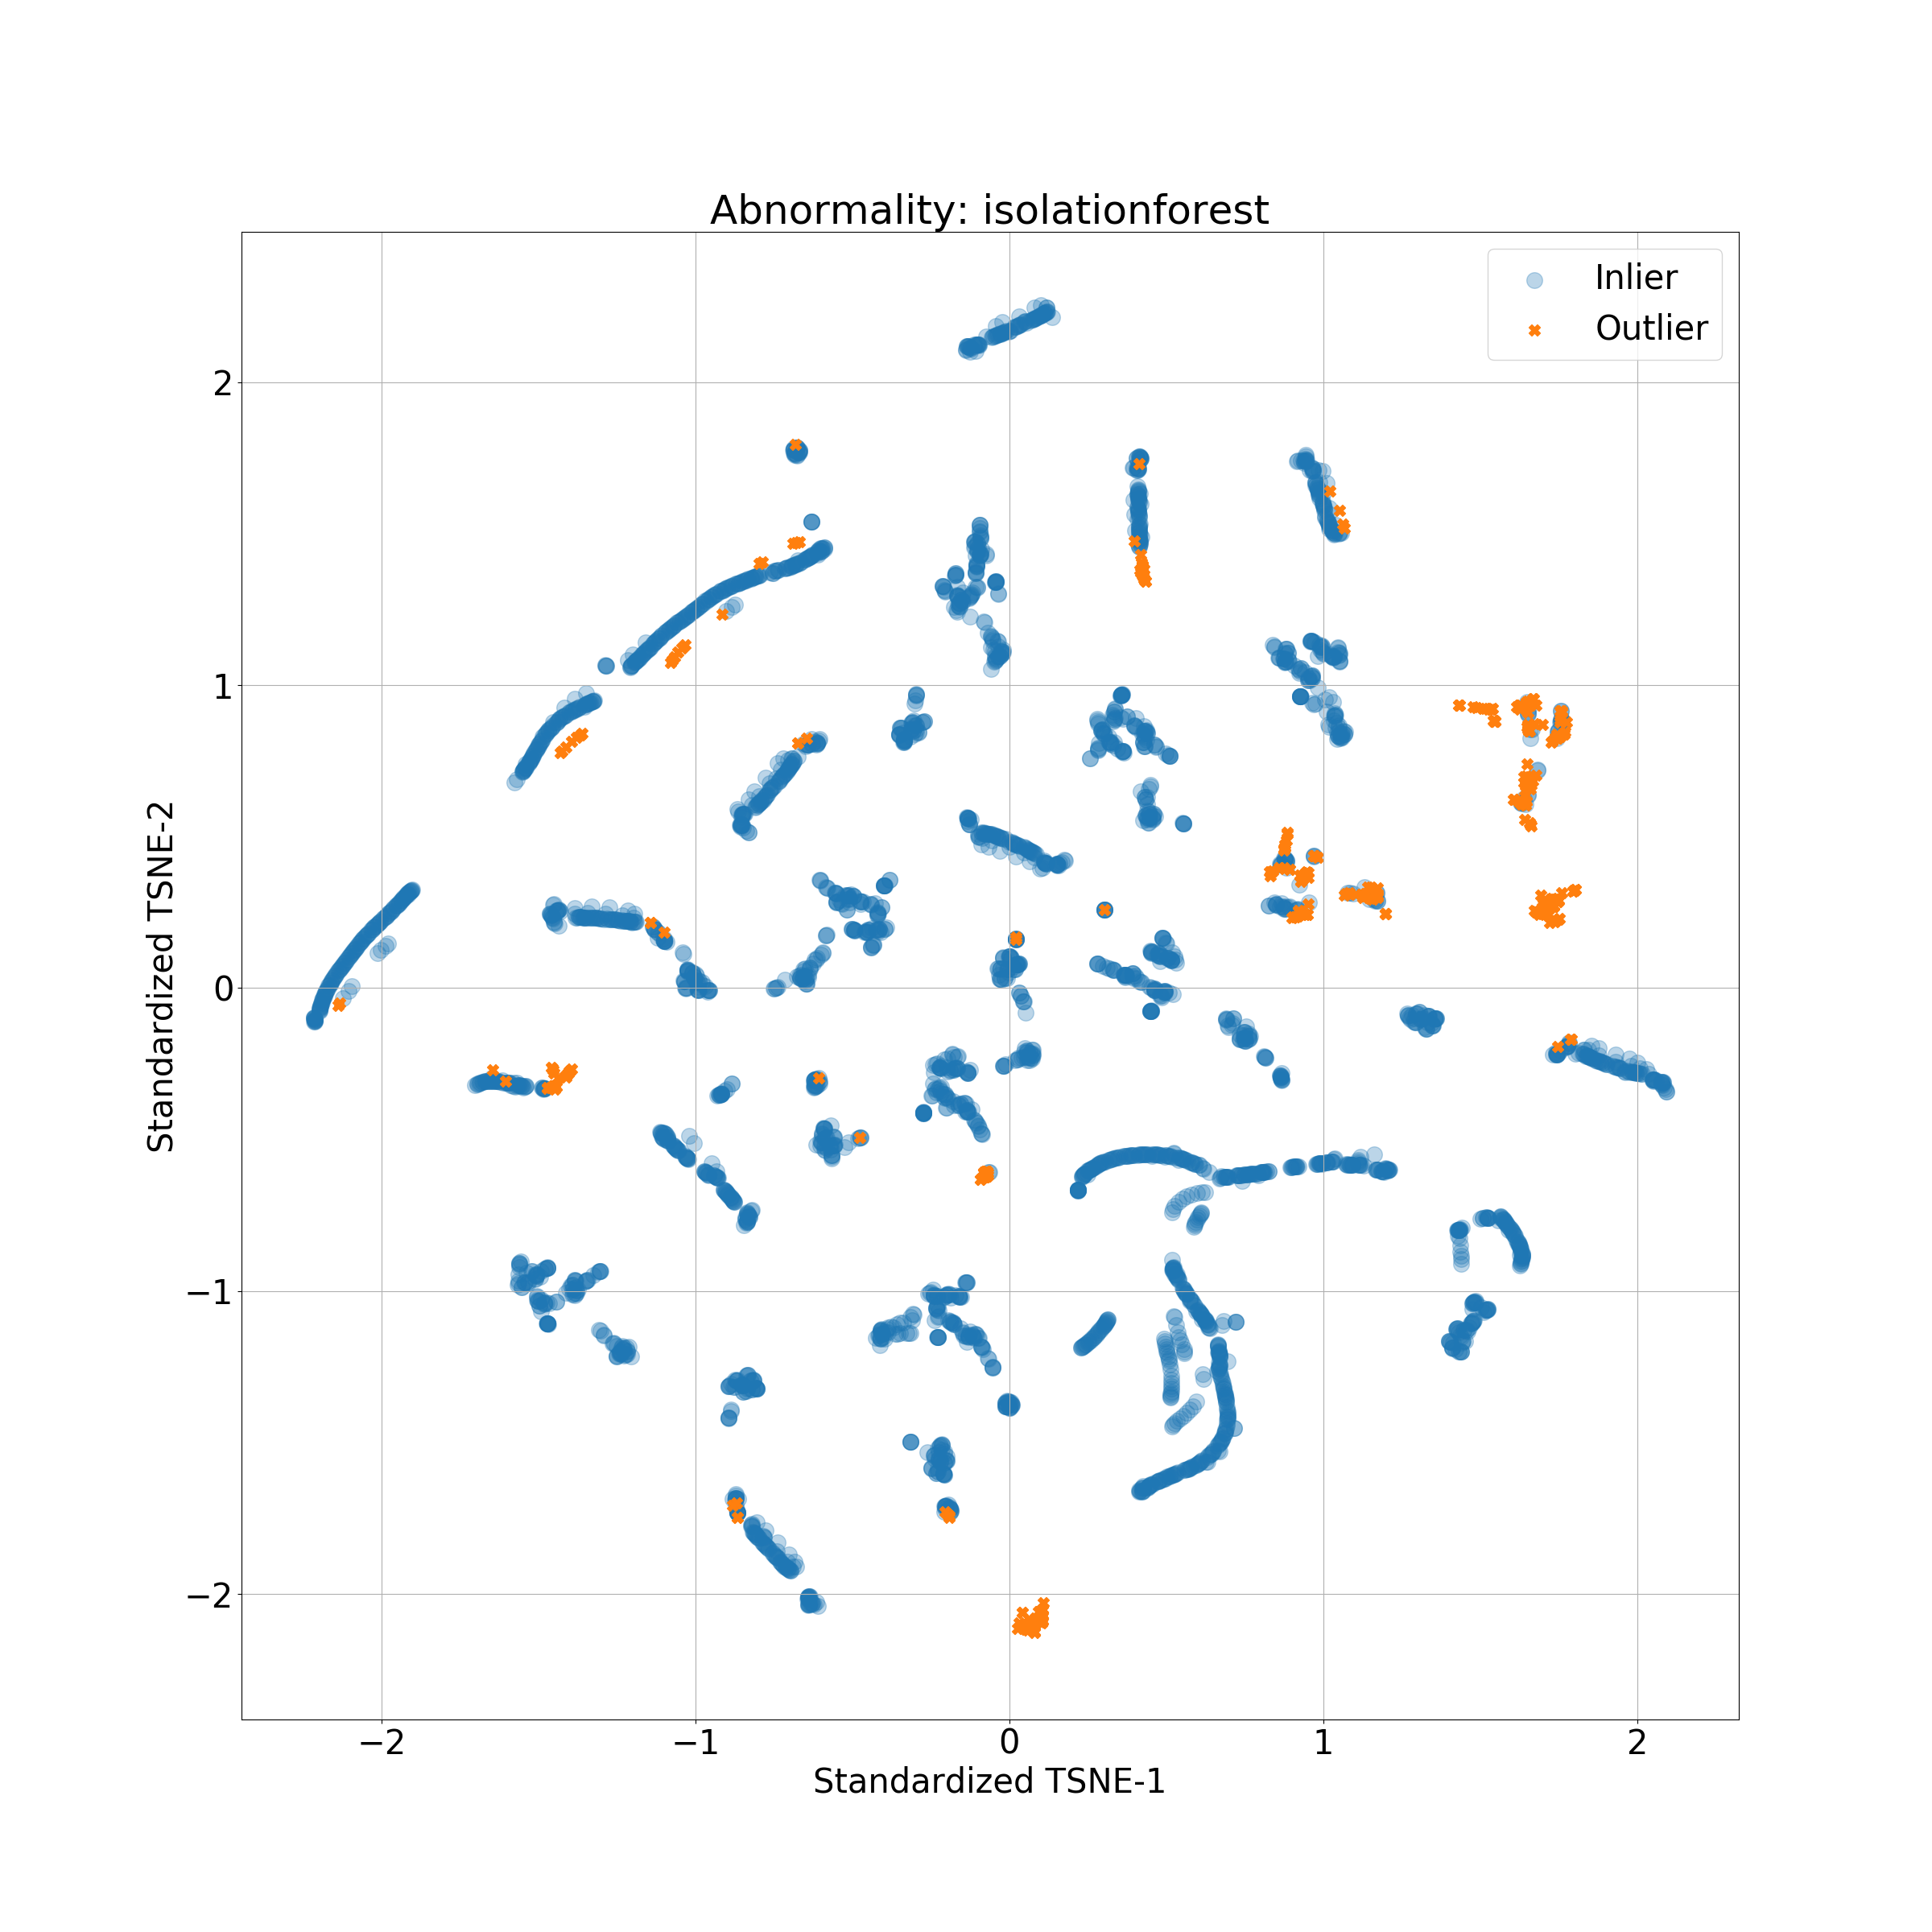
\includegraphics[width=0.3 \linewidth]{figures/outlier3.png}
                        &
                        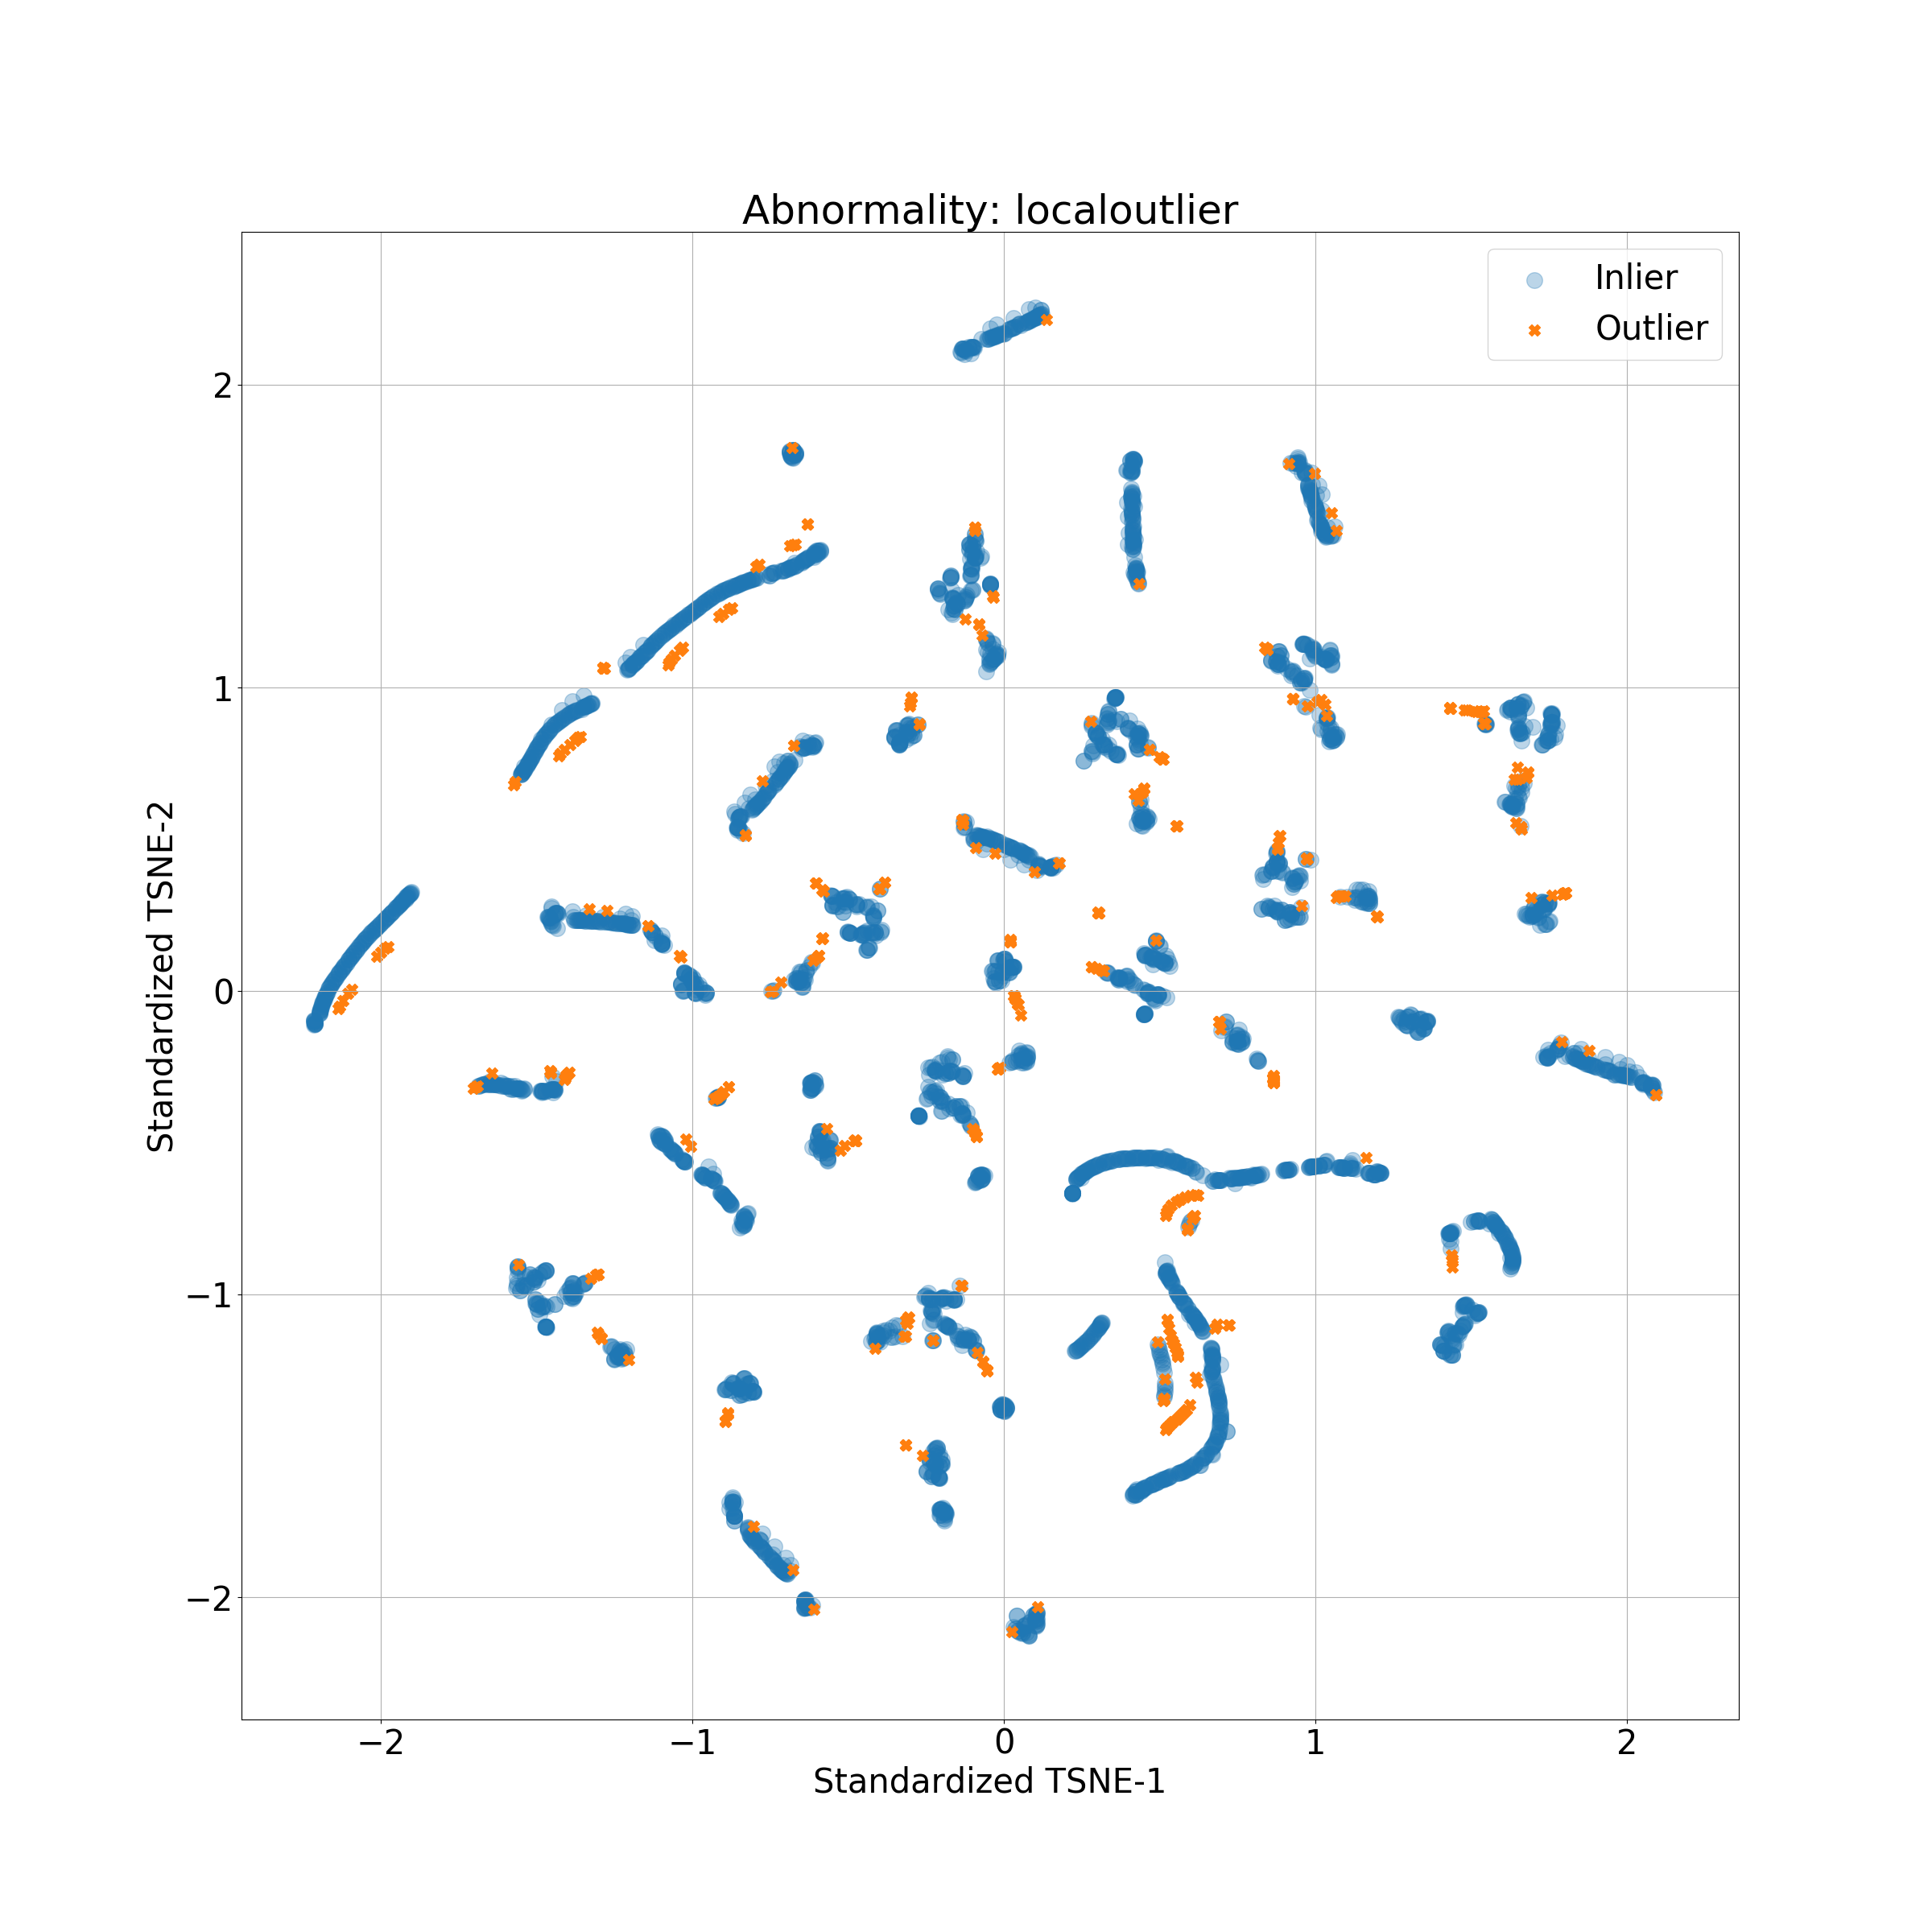
\includegraphics[width=0.3 \linewidth]{figures/outlier4.png}
                        \\
                        
                        \mbox{(c) \textit{IsolationForest}} & \mbox{(d) \textit{LocalOutlierFactor}}\\
                    \end{array}$
                    \caption{Abnormality Founded by Algorithms}
                    \label{fig:abnormal}
                \end{figure}
        
                Abnormality founded is shows as figure \ref{fig:abnormal}. Note that some data were considered as abnormal in multiple algorithms; however, no data were considered as abnormal in all algorithms. Moreover, with the data in figure \ref{fig:abnormal}, we can display the timeline of abnormality as figure \ref{fig:abnormaltime}.
            
                \begin{figure}[htbp]
                    \centering
                    $\begin{array}{cc}
                        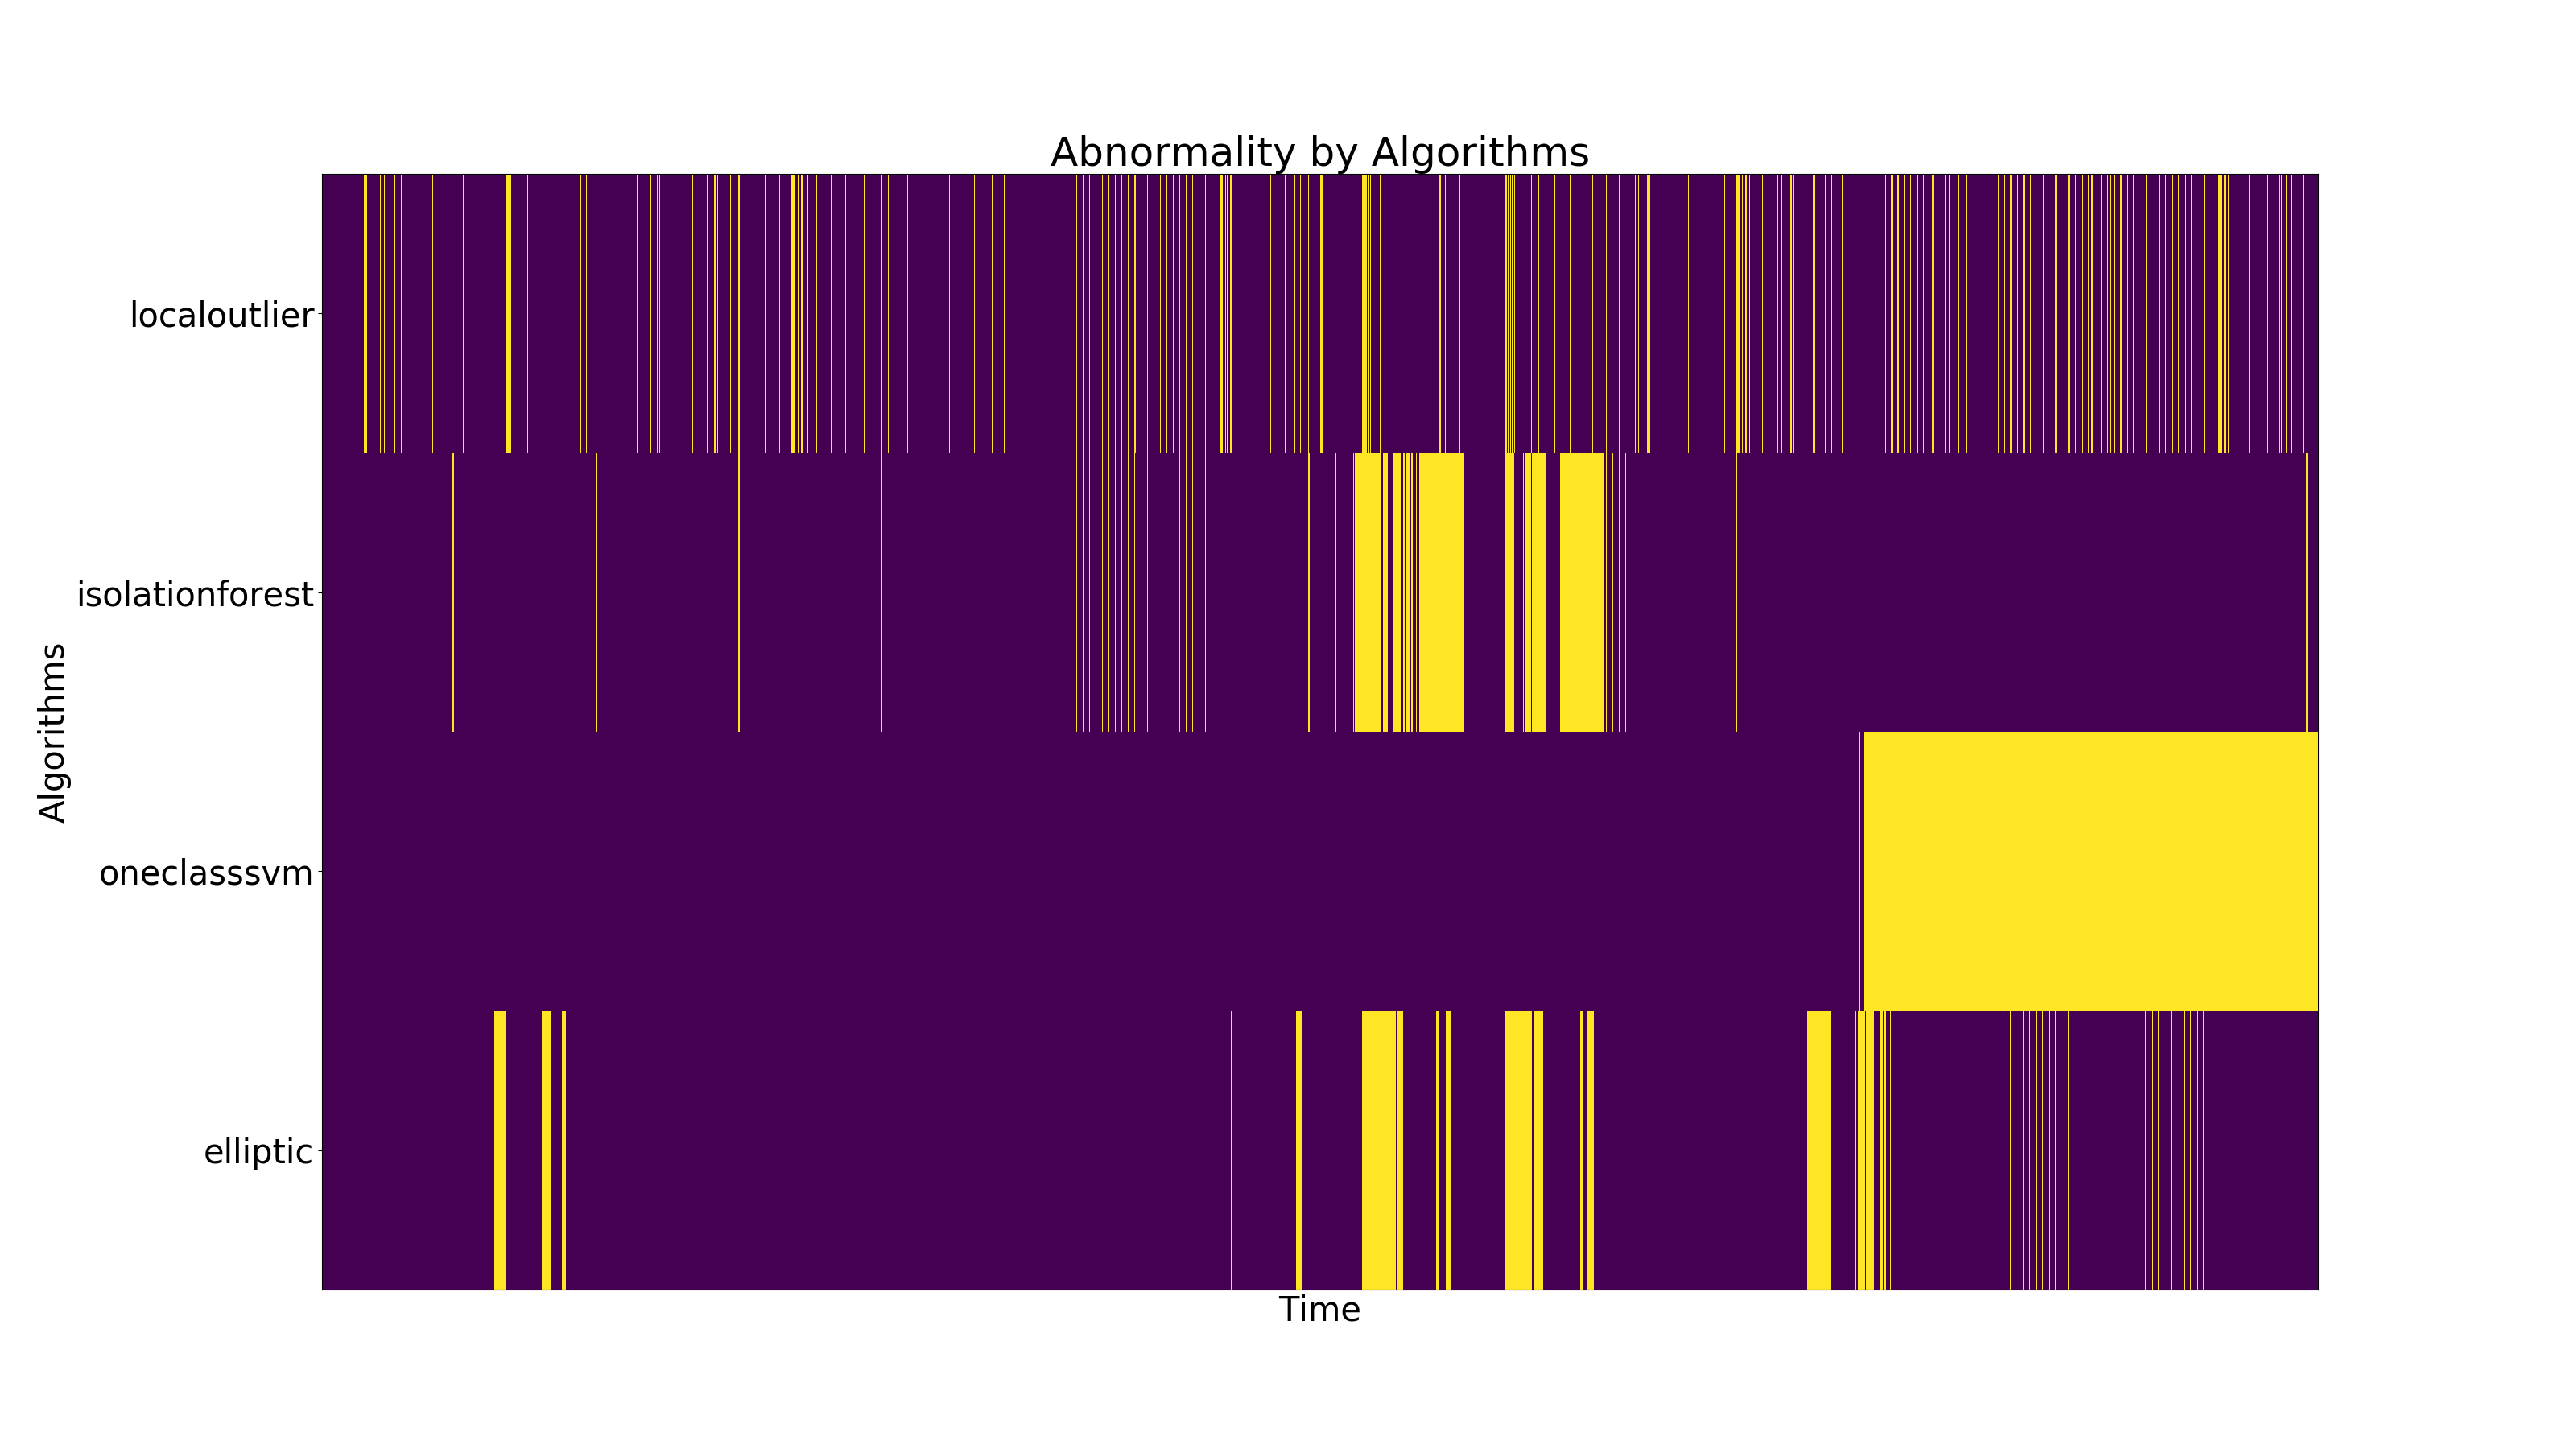
\includegraphics[width=0.4 \linewidth]{figures/normaltime1.png}
                        &
                        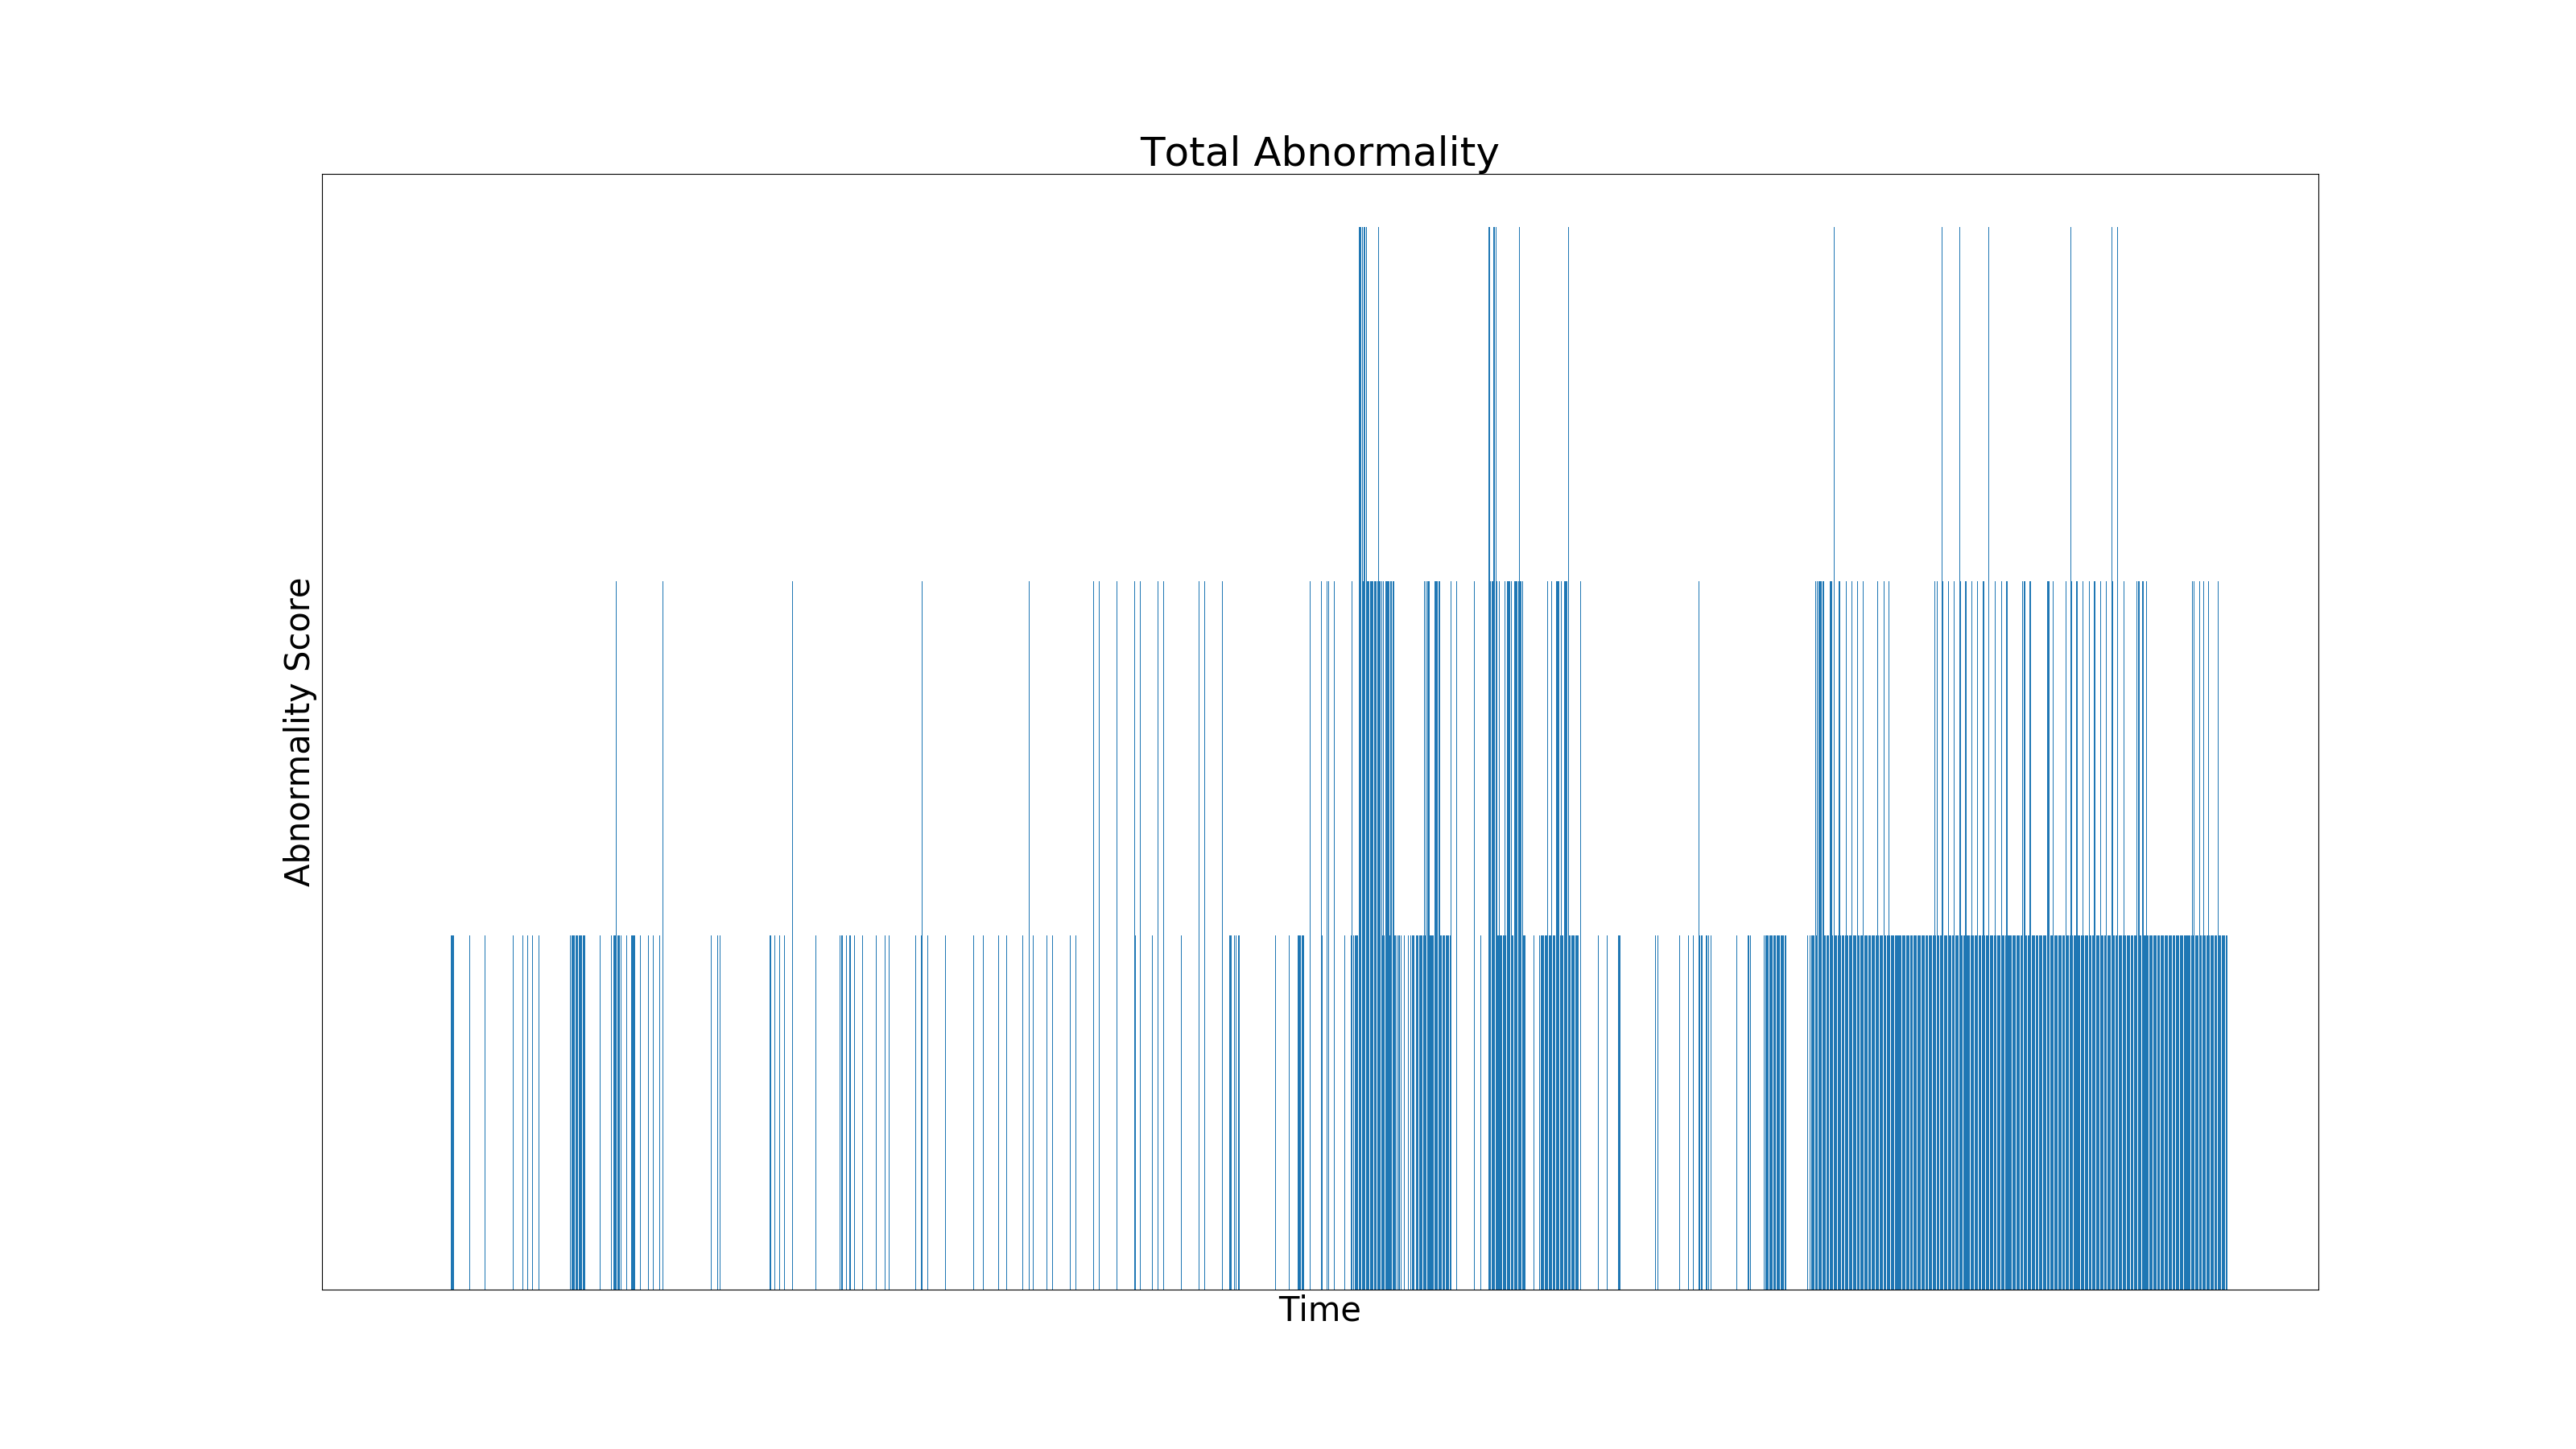
\includegraphics[width=0.4 \linewidth]{figures/normaltime2.png}
                        \\
                        
                        \mbox{(a)} & \mbox{(b)} \\
                    \end{array}$
                    \caption{Abnormality by Timeline}
                    \label{fig:abnormaltime}
                \end{figure}
            
                In the figure \ref{fig:abnormaltime}-(a), we can know that which algorithm consider specific time as abnormal events (yellow marked is abnormal); and, in the figure \ref{fig:abnormaltime}-(b), we can realize that how many algorithms consider specific time as abnormal events. 
        
        \subsection[Question 3]{Describe up to five notable anomalies or unusual events you see in the data. Prioritize those issue that are most likely to represent a danger or a serious issue for building operations.}
            \subsection{General Information of Hazium Concentration}
                In the question 2, we have already found about the abnormality of general building data. Therefore, we do not have same thing twice. However, in the question 3, we need to find a danger or a serious issue for building data. Hence, we suppose that a danger will be related with Hazium concentration.
                
                \begin{figure}[htbp]
                    \centering
                    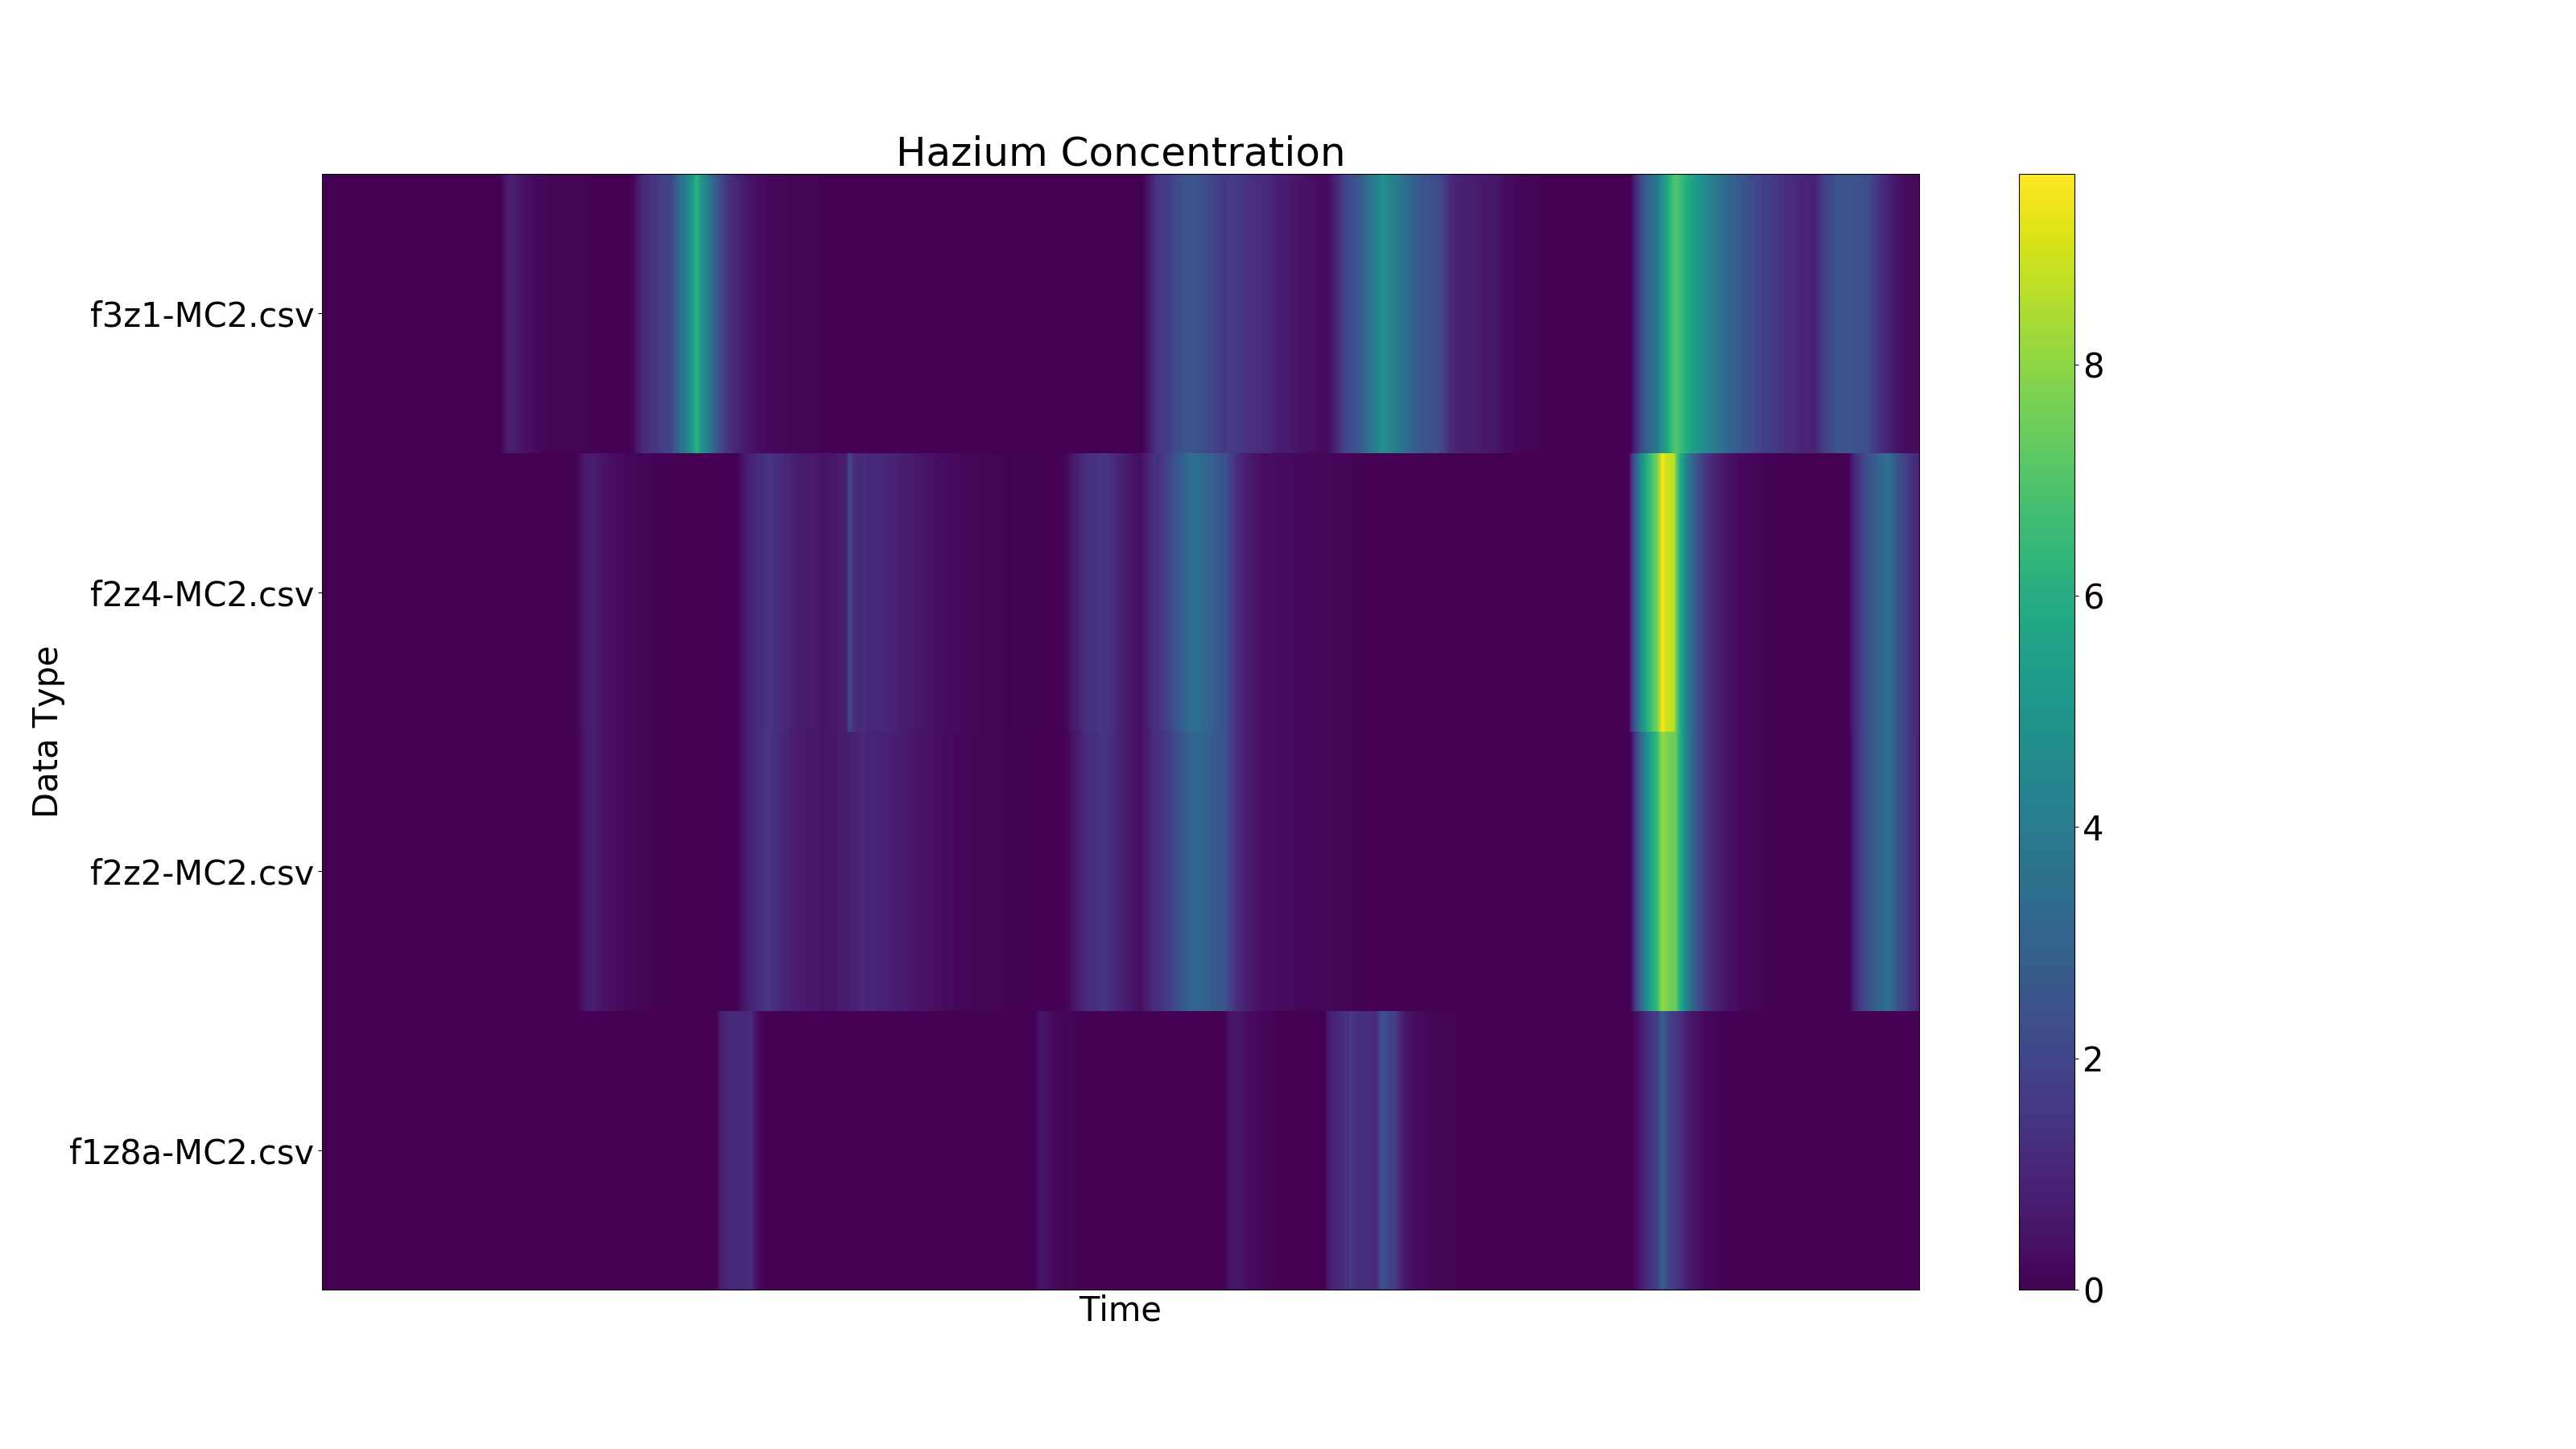
\includegraphics[width=0.4 \linewidth]{figures/hazium.png}
                    \caption{Hazium Data from Different Data Sources}
                    \label{fig:generalhazium}
                \end{figure}
            
                In the figure \ref{fig:generalhazium}, we can see Hazium concentration of many sources. 

            \subsubsection{Workflow}
        
        \subsection[Question 4]{Describe up to three observed relationships between the proximity card data and building data elements. If you find a causal relationship, describe your discovered cause and effect, the evidence you found the support it, and your level of confidence in your assessment of the relationship.}
            \subsubsection{General Information}
            
            \subsubsection{Workflow}
    
    \section{Discussion}
    
    \bibliographystyle{ieeetr}
    \bibliography{reference}
\end{document}